\documentclass[12pt,a4paper,oneside]{JITH}
%\documentclass[12pt,a4paper,twoside]{JITH}

\usepackage{amsmath,amsfonts,mathdots,amssymb,mathtools}
\usepackage{textcomp}
\usepackage{graphicx}
\usepackage[caption=false]{subfig}
\usepackage{svg}
\usepackage{hyperref}
\usepackage{bm}
\usepackage{natbib}
\usepackage{pdfpages}
\usepackage{booktabs}
\usepackage{indentfirst}
\usepackage{float}
\usepackage{tcolorbox}
\usepackage{tikz}
\usetikzlibrary{positioning,arrows,arrows.meta,shapes.geometric,fit,backgrounds,calc}
\usepackage{pgfplots}
\pgfplotsset{compat=1.17}
\definecolor{ForestGreen}{rgb}{0.13,0.55,0.13}
% =====================================================================
% Identidade visual de gráficos, tabelas, quadros e guias de escrita
% Adaptado do template ufal-tesis (OA-RAG / Hossain e Sarıyüce)
% =====================================================================

\usepackage{colortbl}
\usepackage{pifont}
\usepackage{fontawesome5}   % ícones para diagramas e fluxogramas
\usepackage{fvextra}        % listagem de prompts/arquivos nos apêndices
\usepackage{placeins}       % \FloatBarrier: mantém figuras dentro da própria seção
\tcbuselibrary{breakable}
\usetikzlibrary{patterns, shapes.arrows}
\usepgfplotslibrary{groupplots, statistics}

% Quadros numerados por capítulo (Quadro 4.1, 5.1...): \begin{quadro}[label=...]{Título}
\newtcolorbox[auto counter, number within=chapter]{quadro}[2][]{
  colback=gray!5,
  colframe=gray!60,
  fonttitle=\bfseries,
  title={Quadro~\thetcbcounter: #2},
  #1
}

% --- Guias de escrita do esqueleto ------------------------------------
% Para ocultar todos os quadros de roteiro na compilação final, altere
% \guiaescritatrue para \guiaescritafalse.
\newif\ifguiaescrita
\guiaescritafalse
\newcommand{\guiasecao}[1]{%
  \ifguiaescrita
    \begin{tcolorbox}[
      breakable,
      colback=vAzul!4,
      colframe=vAzul!45,
      boxrule=0.5pt,
      arc=2pt,
      left=6pt, right=6pt, top=4pt, bottom=4pt,
      fonttitle=\sffamily\bfseries\footnotesize,
      coltitle=vAzul!80!black,
      colbacktitle=vAzul!10,
      title={Roteiro da Seção (esqueleto a redigir)}
    ]
      \footnotesize\sffamily #1
    \end{tcolorbox}%
  \fi
}

% --- Paleta principal -------------------------------------------------
\definecolor{vAzul}{HTML}{2A78D6}
\definecolor{vVerde}{HTML}{1BAF7A}
\definecolor{vLaranja}{HTML}{EB6834}
\definecolor{vAmbar}{HTML}{EDA100}
\definecolor{vRoxo}{HTML}{4A3AA7}
\definecolor{vVermelho}{HTML}{E34948}
\definecolor{vTeal}{HTML}{2A9D8F}
\definecolor{vCinza}{HTML}{9B9A94}
\definecolor{vNeutro}{HTML}{DDDCD5}

% Cores semânticas sugeridas para vereditos do Judge
\colorlet{corAC}{vVerde}
\colorlet{corWA}{vVermelho}
\colorlet{corCE}{vRoxo}
\colorlet{corRE}{vLaranja}
\colorlet{corTLE}{vAmbar}
\colorlet{corMLE}{vTeal}

% --- Tabelas ----------------------------------------------------------
\colorlet{linhaDestaque}{black!6}
\colorlet{colunaDestaque}{black!8}
\newcommand{\tfirst}[1]{{\color{red!80!black}#1}}
\newcommand{\tsecond}[1]{{\color{blue!80!black}#1}}
\newcommand{\gain}[1]{\;{\color{green!50!black}\ensuremath{\uparrow}\,#1}}
\newcommand{\loss}[1]{\;{\color{red!75!black}\ensuremath{\downarrow}\,#1}}
\newcommand{\cmark}{\ding{51}}
\newcommand{\nomark}{{\color{black!35}--}}
\newcommand{\tcok}{\textcolor{green!50!black}{\ding{51}}}
\newcommand{\tcno}{\textcolor{red!75!black}{\ding{55}}}

% Amostra de cor para legendas
\newcommand{\chip}[1]{\tikz[baseline=-0.6ex]\filldraw[fill=#1, draw=black!40, line width=0.3pt] (0,-0.09) rectangle (0.30,0.09);\hspace{2.5pt}}

% Barra proporcional dentro de célula de tabela (valor em [0,1]):
% \barcell{cor}{valor}{rótulo}
\newcommand{\barcell}[3]{%
  \tikz[baseline=-0.6ex]{%
    \fill[black!5] (0,-0.11) rectangle (1.6,0.11);%
    \fill[#1] (0,-0.11) rectangle ({1.6*#2},0.11);%
    \node[anchor=west, inner sep=0pt, font=\footnotesize] at ({1.6*#2+0.06},0) {#3};%
  }%
}

% --- Posicionamento de figuras ----------------------------------------
\renewcommand{\topfraction}{.92}\renewcommand{\dbltopfraction}{.92}
\renewcommand{\textfraction}{.06}\renewcommand{\floatpagefraction}{.72}

% --- Heatmap de células -----------------------------------------------
% Branco/verde (0) -> amarelo (50) -> vermelho (100); imprime o valor.
\newcommand{\heatmap}[1]{%
    \pgfmathsetmacro{\val}{#1}%
    \pgfmathsetmacro{\r}{ifthenelse(\val<50, \val/50, 1)}%
    \pgfmathsetmacro{\g}{ifthenelse(\val<50, 1, 2-\val/50)}%
    \pgfmathsetmacro{\b}{0}%
    \edef\temp{\noexpand\cellcolor[rgb]{\r,\g,\b}}%
    \temp #1%
}

% --- Número do capítulo em fonte monoespaçada no cabeçalho de abertura -
\usepackage{etoolbox}
\makeatletter
\patchcmd{\@makechapterhead}{\thechapter}{{\ttfamily\fontsize{34}{34}\selectfont\thechapter}}{}{\PackageWarning{estilo-visual}{patch do numero do capitulo falhou}}
\makeatother
  % paleta, macros de gráficos/tabelas e guias do esqueleto

% utf8/T1/babel já são carregados pela classe JITH (ver JITH.cls).
% tcolorbox carrega verbatim internamente, que define \comment; desfazemos a
% definição antes de carregar easyReview para evitar colisão de macros.
\let\comment\relax
\let\endcomment\relax
\setlength{\marginparwidth}{2cm}
\usepackage{easyReview} %% para revisões (\add, \remove, \replace, \comment, \alert)
\setreviewsoff          %% altere para \setreviewson durante revisões

% =====================================================================
% Macros matemáticas e tipográficas do TCC
% =====================================================================

\newcommand{\R}{\mathbb{R}}
\newcommand{\N}{\mathbb{N}}
\newcommand{\E}{\mathbb{E}}

% Notação específica do domínio de benchmark de LLMs
\newcommand{\passat}[1]{\ensuremath{\mathrm{Pass@}#1}}
\newcommand{\veredito}[1]{\texttt{#1}}
\newcommand{\linguagem}[1]{\textsf{#1}}
\newcommand{\promptname}[1]{\texttt{#1}}
\newcommand{\modalidade}[1]{\texttt{#1}}
\newcommand{\bigo}[1]{\ensuremath{\mathcal{O}\!\left(#1\right)}}


\onehalfspacing
\bibliographystyle{plainnat}        % estilo [Autor et al., Ano]

\begin{document}
\sloppy

% % % % % % % % % % % % % % % % % % % % % % % % % % %
% Identificação e Elementos Pré-textuais               %
% % % % % % % % % % % % % % % % % % % % % % % % % % %
\author{Victor Hugo Silva Ângelo}
\email{vhsa@ic.ufal.br}
\docTitle{Avaliação Experimental de LLMs na Resolução de Problemas da Olimpíada Brasileira de Informática: Modalidade Programação, Nível Sênior}

\docType{1} %% TCC=1; Qualificação Mestrado=2; Dissertação=3; Qualificação Doutorado=4; Tese=5

% % % % % % % % % % % % % % % % % % % % % % % % % % % % % %
% Orientação                                                 %
% % % % % % % % % % % % % % % % % % % % % % % % % % % % % %
\orientador{Evandro de Barros Costa}
\tituloOrientador{Prof. Dr.}
%\coorientador{[Nome do(a) Coorientador(a)]}
%\tituloCoorientador{Prof. Dr.}

% % % % % % % % % % % % % % % % % % % % % % % % % % % % % %
% Banca Avaliadora                                           %
% % % % % % % % % % % % % % % % % % % % % % % % % % % % % %
\memberA{[Membro 1 da Banca -- a definir]}
\filiationA{Prof. Dr., IC-UFAL}

\memberB{[Membro 2 da Banca -- a definir]}
\filiationB{Prof. Dr., IC-UFAL}

\memberC{} %% opcional: preencher caso haja 3º membro além do orientador
\filiationC{Prof. Dr., IC-UFAL}

% % % % % % % % % % % % % % % % % % % % % % % % % % % % % %
% Local e Data                                               %
% % % % % % % % % % % % % % % % % % % % % % % % % % % % % %
\setMonth{Novembro}
\setDate{}   %% vazio: imprime só mês e ano; preencher com o dia da defesa
\setYear{2026}
\setLocation{Maceió, Alagoas}


\capa
\folhaDeRosto
\folhaDeAprovacao
\dedicatoria
\epigrafe
% \includepdf{Cap00/FichaCatalografica.pdf}
% \includepdf{Cap00/TCC_avaliacao_assinado.pdf}

\agradecimentos

\resumo
\abstract

\listoffigures
\cleardoublepage

\listoftables
\cleardoublepage

% \simbolos
% \cleardoublepage

\abreviaturas
\cleardoublepage

\tableofcontents
\cleardoublepage

% % % % % % % % % % % % % % % % % % % % % % % % % % %
% Corpo Textual                                        %
% % % % % % % % % % % % % % % % % % % % % % % % % % %
\pagenumbering{arabic}

\pagestyle{myheadings}
\renewcommand{\chaptermark}[1]{\markboth{#1}{}}
\renewcommand{\sectionmark}[1]{\markright{#1}}

\chapter{Introdução}\label{cap:introducao}

O maior desafio da Inteligência Artificial é automatizar tarefas, principalmente no contexto computacional. A cada dia que passa, novas ferramentas que utilizam os Modelos de Linguagem de Grande Porte (LLMs, do inglês \textit{Large Language Models}) estão sendo inseridas no ciclo de desenvolvimento de \textit{software}. Entretanto, será que esses modelos conseguem resolver problemas de programação competitiva? No mundo da programação competitiva, o participante precisa de determinadas habilidades, tais como: interpretar enunciados frequentemente extensos ou ambíguos; projetar algoritmos em relação ao tempo de execução e consumo de memória; extrair requisitos implícitos; e analisar elementos visuais ou padrões da questão.

Essas habilidades exigem atividades cognitivas sofisticadas do competidor, contudo, diante desse cenário, a capacidade dos LLMs na resolução dos problemas da Olimpíada Brasileira de Informática (OBI) pouco foi explorada. Além de ser uma das principais provas aplicadas durante anos no cenário educacional brasileiro para a computação, a OBI destaca-se por desafiar estudantes de diferentes níveis de complexidade. Em paralelo, houve avanços expressivos na geração automática de código executável~\citep{chen2021evaluating, Mendoza2024Comparative} por meio de Processamento de Linguagem Natural, devido às leis de escala~\citep{kaplan2020scaling}. Outro ponto importante é que modelos multimodais com técnicas de processamento de texto e imagens, como o \textit{Visual Instruction Tuning}~\citep{Liu2023VisualIT}, ganharam notoriedade em \textit{benchmarks}~\citep{Fu2023MMEAC,Lu2023MathVistaEM}. Porém, essa abordagem foi pouco explorada em \textit{benchmarks} de programação competitiva.

Embora estudos internacionais e nacionais investiguem o desempenho de LLMs na resolução de problemas algorítmicos e exames educacionais~\citep{chen2021evaluating,zheng2025livecodebench,li2024evaluating,mendonca2024evaluating,viegas2025assessing,almeida2023bluex}, ainda há carência de evidências experimentais sistemáticas sobre o comportamento desses modelos em problemas brasileiros da OBI no \textbf{Nível Sênior} da Modalidade Programação. Esse nível, considerado o mais difícil da competição, combina validação objetiva por juízes automatizados com casos de teste oficiais e ampla variedade algorítmica, configurando um ambiente metodologicamente robusto para analisar como LLMs lidam com múltiplas linguagens de programação, enunciados com imagens, explicitação de limites de recursos e estratégias estruturadas de engenharia de \textit{prompt}.

Em estudo preliminar junto ao grupo de pesquisa \textit{GEMA-LAB} com foco em todos os níveis da Modalidade Programação da OBI em Python e C++~\citep{angelo2026ise}, com disponibilização pública dos artefatos~\citep{obibenchmarking2026,problems2026}, observou-se que a qualidade da geração varia sensivelmente conforme a dificuldade do problema, a presença de contexto visual e o formato de instruções fornecido ao modelo. O presente Trabalho de Conclusão de Curso (TCC) aprofunda e estende essa linha de investigação especificamente para o \textbf{Nível Sênior da OBI}, introduzindo uma avaliação experimental controlada sobre \textbf{cinco linguagens de programação}, \textbf{três modalidades de representação visual} (texto puro, imagem em Base64 e descrição textual estruturada), \textbf{injeção explícita de limites computacionais}, \textbf{técnicas de \textit{prompting}} e uma \textbf{comparação geracional sob paridade de juiz} entre modelos atuais e da geração anterior.

\section{Perguntas de Pesquisa}\label{sec:intro-rqs}

Para investigar de forma sistemática a capacidade de LLMs na resolução de problemas de Nível Sênior da OBI, este trabalho é guiado por cinco perguntas de pesquisa (PP):

\begin{enumerate}
    \item \textbf{PP1 (Desempenho Geral e Variação entre Linguagens):} Qual é a taxa de acerto (\passat{1}, sob decodificação determinística $T = 0$) dos LLMs na resolução textual dos problemas da OBI (Nível Sênior) e como esse desempenho varia entre as cinco linguagens de programação avaliadas (\linguagem{Python}, \linguagem{C}, \linguagem{C++}, \linguagem{Java} e \linguagem{JavaScript})?
    \item \textbf{PP2 (Impacto da Multimodalidade):} Como a presença de imagens nos enunciados influencia o desempenho dos modelos e qual o impacto de diferentes modalidades de representação visual (\modalidade{text}, \modalidade{img} em Base64 e \modalidade{description} textual enriquecida) sobre a taxa de acerto, o perfil de falhas e o consumo de \textit{tokens}?
    \item \textbf{PP3 (Explicitação de Restrições Computacionais):} Qual é o impacto do fornecimento explícito das restrições de tempo (\texttt{time\_limit}) e memória (\texttt{memory\_limit}) no \textit{prompt} sobre o percentual de submissões aceitas e sobre a qualidade algorítmica das soluções geradas na linguagem mais sensível do \textit{baseline}?
    \item \textbf{PP4 (Estratégias de Engenharia de \textit{Prompt}):} Como diferentes estratégias de \textit{prompting} (\textit{Zero-Shot}, \textit{Few-Shot} e \textit{Chain-of-Thought} guiado pela Metodologia de Pólya) impactam a taxa de acerto, a taxonomia de erros e a eficiência econômica (custo por solução aceita) na linguagem mais desafiadora?
    \item \textbf{PP5 (Evolução Geracional sob Paridade de Juiz):} Como os LLMs da geração atual (\textit{Gemini 3.8 Flash} e \textit{GPT-6 Luna}) se comparam aos modelos da geração anterior (\textit{Gemini 3.1 Pro} e \textit{GPT-5.4}) sob protocolo idêntico em \linguagem{Python} \textit{Zero-Shot}?
\end{enumerate}

\section{Objetivo Geral}\label{sec:intro-objetivo}

Avaliar experimentalmente a capacidade de Modelos de Linguagem de Grande Porte na resolução automatizada de problemas de Nível Sênior da Olimpíada Brasileira de Informática (Modalidade Programação), mensurando a influência da linguagem de programação, da informação visual, da explicitação de restrições de execução e de estratégias de engenharia de \textit{prompt} sobre a corretude funcional, a eficiência computacional e econômica, além da evolução entre gerações de modelos sob o mesmo protocolo de julgamento.

\subsection{Objetivos Específicos}\label{sec:intro-objetivos-esp}

Para alcançar o objetivo geral e responder às perguntas de pesquisa, definem-se os seguintes objetivos específicos:

\begin{enumerate}
    \item Estruturar e validar, por meio de execução oráculo das soluções de referência, uma base padronizada de 125 problemas do Nível Sênior da OBI (2016--2025) contendo enunciados, metadados, imagens e 4.681 casos de teste oficiais;
    \item Evoluir o \textit{pipeline} automatizado e reprodutível de \textit{benchmarking} e julgamento local multilinguagem capaz de submeter problemas via API, extrair o código gerado e mensurar vereditos, tempo de CPU, uso de memória, \textit{tokens} e custo financeiro;
    \item Avaliar e comparar o desempenho (\passat{1}) e a taxonomia de falhas de múltiplos LLMs (\textbf{DeepSeek v4.1 Flash}, \textbf{Gemini 3.8 Flash} e \textbf{GPT-6 Luna}) nas linguagens \linguagem{Python}, \linguagem{C}, \linguagem{C++}, \linguagem{Java} e \linguagem{JavaScript};
    \item Investigar o efeito da presença de figuras nos enunciados e comparar as modalidades \modalidade{text}, \modalidade{img} (Base64) e \modalidade{description} nas 46 questões com imagens;
    \item Mensurar o impacto da inclusão explícita dos limites de tempo e memória no \textit{prompt} sobre a linguagem com menor desempenho no \textit{baseline};
    \item Comparar estratégias de engenharia de \textit{prompt} (\textit{Zero-Shot}, \textit{Few-Shot} e \textit{Chain-of-Thought} baseado na heurística de Pólya);
    \item Comparar o avanço entre gerações nas famílias Google (\textbf{Gemini 3.1 Pro} versus \textbf{Gemini 3.8 Flash}) e OpenAI (\textbf{GPT-5.4} versus \textbf{GPT-6 Luna}) sob protocolo idêntico em \linguagem{Python} \textit{Zero-Shot}, reavaliando as soluções anteriores no mesmo juiz local adotado neste trabalho.
\end{enumerate}

\section{Relevância do Trabalho}\label{sec:intro-relevancia}

A relevância deste trabalho manifesta-se em três dimensões complementares. No plano \textbf{científico}, o estudo fornece evidência empírica controlada em língua portuguesa sobre capacidades e limites de LLMs em raciocínio algorítmico de nível sênior, superando o viés de avaliações restritas a conjuntos em inglês ou a uma única linguagem de programação. No plano \textbf{metodológico e de Engenharia de \textit{Software}}, o paralelo entre programação competitiva e desenvolvimento de sistemas, no qual a interpretação de enunciados e figuras reflete a modelagem de requisitos e a validação contra casos extremos equivale a testes unitários rigorosos, é operacionalizado por um arcabouço reproduzível com juiz local multilinguagem e telemetria detalhada de custo e verbosidade. Por fim, no plano \textbf{educacional e prático}, compreender onde e por que modelos falham (como erros de E/S, sobre-engenharia ou alucinações lógicas) oferece subsídios concretos para professores, estudantes e projetistas de tutores inteligentes que buscam integrar LLMs como mediadores pedagógicos sem substituir o raciocínio humano na preparação para a Olimpíada Brasileira de Informática~\citep{priyanka2025development,peng2025enhancing}.

\section{Organização do Trabalho}\label{sec:intro-organizacao}

O restante deste trabalho está estruturado da seguinte maneira:
\begin{itemize}
    \item O \textbf{Capítulo~\ref{cap:relacionados}} revisa os trabalhos relacionados sobre avaliação de LLMs em programação competitiva, multimodalidade, engenharia de \textit{prompt} e exames brasileiros;
    \item O \textbf{Capítulo~\ref{cap:fundamentacao}} apresenta a fundamentação teórica acerca de LLMs, decodificação, técnicas de \textit{prompting}, estrutura da OBI e métricas de avaliação;
    \item O \textbf{Capítulo~\ref{cap:metodologia}} detalha a construção e validação da base de dados, a arquitetura do \textit{benchmark} desenvolvido e o desenho experimental para cada pergunta de pesquisa;
    \item O \textbf{Capítulo~\ref{cap:resultados}} apresenta e discute os resultados experimentais obtidos para PP1 a PP5, bem como as ameaças à validade;
    \item O \textbf{Capítulo~\ref{cap:conclusao}} sintetiza as conclusões, contribuições e direções para trabalhos futuros.
\end{itemize}

\cleardoublepage

\chapter{Trabalhos Relacionados}\label{cap:relacionados}

Para verificar como a área de estudo tem sido explorada, foi conduzida uma revisão sistemática da literatura com o objetivo de identificar artigos da comunidade científica. O protocolo de busca foi estruturado com base no \textit{Population}, \textit{Intervention}, \textit{Comparison}, \textit{Outcome}, \textit{Context} (PICOC), resultando na seguinte \textit{string} de busca:

\begin{quote}
\small\ttfamily
("competitive programming" OR "competition-level" OR "programming contest*" OR "programming competition*" OR "informatics olympiad" OR "algorithmic problem solving" OR "programming exercises")
AND
("large language model*" OR "language model*" OR "LLM" OR "LLMs" OR "MLLM" OR "MLLMs" OR "multimodal")
AND
("benchmark*" OR "evaluat*" OR "assess*" OR "online judge*" OR "codeforces" OR "correctness")
\end{quote}

Por meio dessa consulta, foram encontrados 664 artigos nas plataformas OpenAlex e arXiv. Desses trabalhos, após a triagem e aplicação dos critérios de seleção, apenas 5 foram selecionados por meio da leitura do título e do resumo, cujo objetivo principal era avaliar \textit{benchmarks}. Por fim, foram realizadas pesquisas manuais complementares sobre os temas de dimensões linguísticas e multimodais, engenharia de \textit{prompt} e avaliações no contexto brasileiro e da OBI, totalizando 21 artigos que ajudam a posicionar este trabalho frente aos estudos existentes.

\section{LLMs na Resolução de Problemas de Programação Competitiva}\label{sec:rel-comp-prog}

Como os LLMs são não determinísticos, os estudos trazem a métrica $\passat{k}$ sobre o contexto do modelo Codex em HumanEval~\citep{chen2021evaluating}. Essa é a consolidação da avaliação funcional de código gerado por LLMs mediante execução contra casos de teste unitários. Em seguida, o AlphaCode~\citep{li2022competition} trouxe a visão de geração de soluções competitivas em plataformas de alto rigor algorítmico como Codeforces, aplicando os estudos dessa categoria na programação competitiva, exigindo amostragem em larga escala e filtragem por casos de teste. 

Mais recentemente, pesquisas têm explorado problemas de olimpíadas e competições como avaliadores exigentes da capacidade de raciocínio de modelos de fronteira~\citep{huang2024competition,li2024evaluating,zheng2025livecodebench}. \citet{li2024evaluating} têm como objetivo analisar, em perspectiva multiano e multinível, o desempenho de LLMs em programação competitiva, evidenciando que, à medida que o grau de dificuldade aumenta, as soluções geradas não conseguem acompanhar, mostrando que ainda existem lacunas a serem exploradas. Na mesma direção, o \textit{LiveCodeBench Pro}~\citep{zheng2025livecodebench} mostra como medalhistas de olimpíadas analisam falhas sutis em soluções geradas por LLMs, mostrando que modelos têm alta taxa de acerto em questões rotineiras, mas falham em questões sofisticadas. Apesar da relevância desses estudos, sua ênfase está em enunciados da língua inglesa e em um conjunto restrito de linguagens (Python ou C++).

\section{Multimodalidade, Restrições e Impacto da Linguagem de Programação}\label{sec:rel-dimensoes}

Com a técnica \textit{Visual Instruction Tuning}~\citep{Liu2023VisualIT} em evidência, passou a ganhar destaque uma área de pesquisa que busca utilizar a multimodalidade dos modelos para interpretação conjunta de texto e elementos visuais~\citep{Fu2023MMEAC}. Em contextos diferentes da programação competitiva, \textit{benchmarks} como MathVista~\citep{Lu2023MathVistaEM} e MMMU~\citep{Yue2023MMMUAM} demonstraram que figuras e diagramas adicionam camadas relevantes de interpretação espacial e simbólica.

Na Engenharia de \textit{Software}, a avaliação de LLMs tem avançado para especificação de requisitos e automação de testes~\citep{Mendoza2024Comparative,Silva2025LLMs}, bem como para a resolução de problemas visuais em repositórios reais, como no \textit{SWE-bench Multimodal}~\citep{Yang2024SWEbenchMD}. Nesse sentido, na programação competitiva a criação desses tipos de testes é interessante para avaliar o impacto da linguagem de programação em relação à sintaxe e à semântica. Entretanto, poucos estudos isolam o impacto de representações visuais em problemas competitivos multilinguagem, tampouco investigam como a explicitação de limites de tempo e memória altera o comportamento algorítmico em linguagens compiladas de baixo nível como \linguagem{C}.

\section{Engenharia de \texorpdfstring{\textit{Prompt}}{Prompt} e Raciocínio Heurístico em Código}\label{sec:rel-prompt}

Como já foi mencionado, as leis de escala para modelos neurais de linguagem~\citep{kaplan2020scaling} em conjunto com as arquiteturas abertas otimizadas em grandes volumes de dados~\citep{touvron2023llama} viabilizaram capacidades emergentes de aprendizado em contexto. Em \citet{wei2021finetuned} foi evidenciada a capacidade de modelos ajustados por instruções operarem em regime \textit{Zero-Shot}, enquanto \citet{brown2020language} demonstraram que exemplos fornecidos diretamente no \textit{prompt} (\textit{Few-Shot}) conseguem ter impacto direto no formato e no raciocínio do modelo sem atualização de pesos.

Em busca de conhecer melhor a engenharia de \textit{prompt}, foi encontrado um guia sistemático de engenharia de \textit{prompt}~\citep{dair2025prompt} que consolidou estratégias como \textit{Few-Shot} e cadeia de pensamento (\textit{Chain-of-Thought} - CoT)~\citep{wei2022chain} para decompor problemas complexos em etapas intermediárias explícitas antes da emissão da resposta final. Para este estudo, na geração de código para juízes automáticos, a ancoragem em exemplos \textit{Few-Shot} tem se mostrado relevante para prevenir falhas de formatação de entrada e saída padrão, enquanto estratégias CoT estruturadas visam reduzir erros lógicos de modelagem.

\section{Avaliação de LLMs em Português, Educação e na OBI}\label{sec:rel-obi}

No contexto brasileiro, diversos estudos têm avaliado LLMs em exames vestibulares e acadêmicos de computação, incluindo o ENEM e provas universitárias no \textit{BLUEX}~\citep{nunes2023evaluating,almeida2023bluex}, o exame nacional de graduação em Computação (ENADE)~\citep{mendonca2024evaluating} e o exame de pós-graduação POSCOMP~\citep{viegas2025assessing}. Do ponto de vista educacional, compreender as dificuldades de resolução algorítmica é fundamental para construir sistemas de tutoria inteligente que apoiem estudantes em relação às lacunas de aprendizagem~\citep{priyanka2025development,peng2025enhancing}. Porém, ainda é um desafio fazer com que os LLMs não entreguem as respostas prontas, para que os estudantes desenvolvam o próprio raciocínio.

Em contrapartida, no contexto da OBI, \citet{alcantara2025assessing} avaliaram o modelo Llama 3 na geração automática de soluções em C++ para exercícios de programação da OBI, reportando taxa de acerto global de 30,4\% e destacando dificuldades dos modelos com limites estritos de tempo e memória, bem como degradação de desempenho quando o contexto visual dos enunciados é omitido. Em trabalho anterior a este TCC, conduzido em conjunto com o grupo de pesquisa \textit{GEMA-LAB}~\citep{angelo2026ise}, estruturou-se um repositório de questões extraídas da OBI~\citep{problems2026} e propôs-se uma versão inicial da arquitetura experimental automatizada~\citep{obibenchmarking2026}. Nesse estudo preliminar, foram avaliados cinco MLLMs proprietários em Python (\textit{zero-shot}) sobre 181 problemas da OBI com imagens em Base64 versus enunciados puramente textuais, observando ganhos do contexto visual em questões fáceis e em casos de borda nas questões avançadas (grafos e programação dinâmica) na maioria dos modelos, embora ainda insuficientes para superar barreiras de raciocínio algorítmico complexo.

O TCC expande substancialmente essa linha de pesquisa ao concentrar-se no \textbf{Nível Sênior da OBI} (125 problemas de 2016 a 2025, com 4.681 casos de teste validados por oráculo) e investigar dimensões ainda não avaliadas em conjunto: (i) comparação cruzada em \textbf{cinco linguagens} (Python, C, C++, Java e JavaScript); (ii) contraste controlado em C++ entre \textbf{texto puro}, \textbf{imagem em Base64} e \textbf{descrição textual estruturada}; (iii) análise do efeito da \textbf{explicitação de limites de tempo e memória} na linguagem mais sensível (\linguagem{C}); (iv) comparação de \textbf{Zero-Shot}, \textbf{Few-Shot} e \textbf{Chain-of-Thought guiado pela Metodologia de Pólya}, incluindo análise de custos e diagnóstico de artefatos de extração; e (v) \textbf{comparação geracional sob paridade de juiz} entre modelos da geração atual (\textit{Gemini 3.8 Flash} e \textit{GPT-6 Luna}) e seus antecessores avaliados no estudo preliminar (\textit{Gemini 3.1 Pro} e \textit{GPT-5.4}) em \linguagem{Python} \textit{Zero-Shot}.

\section{Síntese Comparativa}\label{sec:rel-sintese}

A Tabela~\ref{tab:rel-comparativo} apresenta as principais características dos estudos relacionados frente à abordagem proposta neste trabalho.

\begin{table}[!htbp]
\centering
\caption[Síntese comparativa dos trabalhos relacionados]{Síntese comparativa entre trabalhos relacionados e o presente estudo.}
\label{tab:rel-comparativo}
\small
\resizebox{\textwidth}{!}{%
\begin{tabular}{lcccccc}
\toprule
Trabalho & Base / Idioma & Linguagens & Multimodal & Limites & Estratégias de \textit{Prompt} & Custo \\
\midrule
\citet{chen2021evaluating}     & HumanEval / EN       & 1 (Python)     & \nomark & \nomark & Zero-Shot              & \nomark \\
\citet{li2022competition}      & CodeContests / EN    & C++, Python    & \nomark & \cmark  & Amostragem massiva     & \nomark \\
\citet{zheng2025livecodebench} & Competições / EN     & C++, Python    & \nomark & \cmark  & Padrão                 & \nomark \\
\citet{mendonca2024evaluating} & ENADE / PT-BR        & -- (Q\&A)      & \cmark  & \nomark & Zero-Shot              & \nomark \\
\citet{viegas2025assessing}    & POSCOMP / PT-BR      & -- (Q\&A)      & \nomark & \nomark & Zero-Shot              & \nomark \\
\citet{alcantara2025assessing} & OBI / PT-BR          & 1 (C++)        & \nomark & \cmark  & Zero-Shot              & \nomark \\
\citet{angelo2026ise}          & OBI / PT-BR          & 1 (Python)     & \cmark  & \nomark & Zero-Shot              & \cmark \\
\midrule
\rowcolor{linhaDestaque}\textbf{Este trabalho} & \textbf{OBI Sênior / PT-BR} & \textbf{5} & \tcok & \tcok & \textbf{ZS / FS / CoT-Pólya} & \tcok \\
\bottomrule
\end{tabular}%
}
\par\smallskip{\footnotesize \tcok: contemplado integralmente (incluindo modalidade descritiva); \cmark: contemplado parcialmente; \nomark: não contemplado.}
\end{table}

\cleardoublepage

\chapter{Fundamentação Teórica}\label{cap:fundamentacao}

Este capítulo tem como objetivo apresentar os conceitos teóricos e técnicos que sustentam o desenho experimental deste trabalho, abrangendo a arquitetura e a decodificação de Modelos de Linguagem de Grande Porte, técnicas de engenharia de \textit{prompt}, a estrutura da Olimpíada Brasileira de Informática e os critérios de avaliação adotados por juízes automatizados.

\section{Modelos de Linguagem de Grande Porte}\label{sec:fund-llms}

\subsection{Arquitetura \textit{Transformer} e Pré-treinamento}\label{sec:fund-transformer}

Os Modelos de Linguagem de Grande Porte (LLMs) modernos baseiam-se na arquitetura \textit{Transformer}, proposta por \citet{vaswani2017}, cujo mecanismo de autoatenção permite relacionar diferentes partes do texto (divididas em \textit{tokens}) em paralelo, capturando dependências de longo alcance sem necessidade de recorrência sequencial. Com o avanço das leis de escala que relacionam quantidade de parâmetros, volume de dados e poder computacional~\citep{kaplan2020scaling}, aliado ao pré-treinamento em grandes bases de texto e código-fonte e ao posterior ajuste por instruções e alinhamento humano~\citep{ouyang2022,wei2021finetuned,touvron2023llama}, esses modelos passaram a gerar código-fonte funcional diretamente a partir de enunciados em linguagem natural.

No entanto, por operarem de forma autorregressiva, prevendo a resposta \textit{token} a \textit{token}, da esquerda para a direita, os LLMs apresentam limitações intrínsecas: quando uma decisão estrutural ou modelagem de estado incorreta é assumida no início da geração do código, o modelo tende a propagá-la até o fim da mesma iteração. Além disso, o texto de entrada e saída é limitado pela janela de contexto, e o consumo de \textit{tokens} impacta diretamente a latência e o custo financeiro das requisições via API. Outro ponto relevante refere-se aos modelos do tipo \textit{thinking}, que atenuam parte desse problema ao raciocinar e revisar o código antes da resposta final, embora ao custo de um maior consumo de \textit{tokens}.

\subsection{Parâmetros de Decodificação e Determinismo}\label{sec:fund-decodificacao}

No intuito de manter a fidelidade do estudo, foi necessário controlar a geração autorregressiva de \textit{tokens}, que é regulada por hiperparâmetros de decodificação, destacando-se a temperatura $T \ge 0$, responsável por reescalar os \textit{logits} antes da função \textit{softmax}. Quando $T > 0$ (como $T = 1{,}0$), a amostragem introduz aleatoriedade, permitindo explorar múltiplas soluções candidatas para um mesmo problema. Por outro lado, o ajuste $T = 0$ corresponde à decodificação gulosa (\textit{greedy decoding}), na qual o modelo escolhe de forma determinística o \textit{token} de maior probabilidade a cada passo.

Neste trabalho, adota-se $T = 0{,}0$ com parâmetros de amostragem padrão para estabelecer uma linha de base estável e reprodutível. Isso permite comparar o efeito de cada variável do estudo (linguagem de programação, modalidade visual, limites de recursos e estratégia de \textit{prompt}) e aproxima o experimento de uma competição real, na qual o participante submete uma única solução final ao avaliador automático.

\subsection{Modelos Multimodais de Visão e Linguagem}\label{sec:fund-multimodal}

Com a introdução do \textit{Visual Instruction Tuning}~\citep{Liu2023VisualIT}, arquiteturas de linguagem foram acopladas a codificadores visuais, dando origem aos Modelos Multimodais de Visão e Linguagem (VLMs/MLLMs). Esses modelos recebem entradas híbridas compostas por texto e imagens, tipicamente codificadas em Base64 ou URLs de dados em chamadas de API, permitindo interpretar diagramas, matrizes visuais, grafos ilustrados e esquemas geométricos~\citep{Fu2023MMEAC,Lu2023MathVistaEM}.

Contudo, o processamento direto de imagens eleva substancialmente a contagem de \textit{tokens} de entrada e pode introduzir ruído na etapa de extração de código. Uma alternativa intermediária consiste em substituir as referências visuais por descrições textuais estruturadas e detalhadas das figuras (\modalidade{description}), preservando a informação espacial em forma puramente textual para reduzir sobrecarga de contexto e ampliar a compatibilidade com modelos focados em texto.

\section{Engenharia de \texorpdfstring{\textit{Prompt}}{Prompt}}\label{sec:fund-prompt}

\subsection{Aprendizado \textit{Zero-Shot} e \textit{Few-Shot} em Contexto}\label{sec:fund-fewshot}

A engenharia de \textit{prompt} estuda a formulação sistemática de instruções para orientar o comportamento de LLMs sem alteração de seus pesos~\citep{dair2025prompt}. Na estratégia \textbf{\textit{Zero-Shot}}~\citep{wei2021finetuned}, o modelo recebe apenas a definição do papel (\textit{persona}), o enunciado do problema e as restrições de formatação da resposta, dependendo apenas do conhecimento adquirido durante o seu pré-treinamento, sem exemplos prévios de resolução.

Já a estratégia \textbf{\textit{Few-Shot}}, consolidada por \citet{brown2020language}, fornece ao modelo exemplos de entrada e saída esperada dentro do próprio contexto do \textit{prompt}. Em programação competitiva, esses exemplos ajudam o modelo a seguir o padrão correto de sintaxe e de E/S padrão (\texttt{stdin}/\texttt{stdout}), orientando convenções como tipos inteiros de 64 bits (\texttt{long long}) para prevenção de \textit{overflow}, leitura eficiente e indexação segura em vetores e grafos.

\subsection{\textit{Chain-of-Thought} e a Metodologia Heurística de Pólya}\label{sec:fund-polya}

A técnica de cadeia de pensamento (\textbf{\textit{Chain-of-Thought} -- CoT})~\citep{wei2022chain} induz o modelo a explicitar etapas intermediárias de raciocínio antes de emitir a solução final. Para estruturar esse processo em problemas algorítmicos, este trabalho integra o CoT ao método heurístico clássico de George Pólya~\citep{polya1945}, organizado em quatro fases encadeadas:

\begin{enumerate}
    \item \textbf{Compreensão:} identificação do objetivo central, formato exato de entrada e saída, limites numéricos e casos de borda ($N = 0, 1$, valores negativos, risco de \textit{overflow} acima de $2 \times 10^9$);
    \item \textbf{Planejamento:} seleção da técnica algorítmica adequada (algoritmo guloso, programação dinâmica, grafos, busca binária, dois ponteiros), escolha de estruturas de dados e análise assintótica $\bigo{\cdot}$ compatível com os limites;
    \item \textbf{Codificação (Execução):} implementação completa e autocontida do programa dentro de um bloco Markdown delimitado;
    \item \textbf{Teste:} validação ``mental'' passo a passo frente aos exemplos do enunciado e aos casos de borda levantados na primeira etapa.
\end{enumerate}

\section{Programação Competitiva e a Olimpíada Brasileira de Informática}\label{sec:fund-obi}

\subsection{Estrutura da OBI e o Nível Sênior}\label{sec:fund-obi-senior}

A OBI, organizada pela Sociedade Brasileira de Computação (SBC) em parceria com a Unicamp, é a principal competição brasileira voltada ao estímulo do pensamento computacional e da resolução de problemas algorítmicos~\citep{obi2026}. A competição divide-se nas modalidades Iniciação e Programação, abrangendo, na modalidade Programação, os níveis Júnior, 1, 2 e \textbf{Sênior}, sendo este último destinado a estudantes ingressantes no ensino superior.

Os problemas do Nível Sênior distribuem-se por fases seletivas progressivas (Fase Local/Fase 1, Fase Estadual/Fase 2 e Fase Nacional/Fase 3) e contemplam tópicos avançados da ementa oficial da OBI~\citep{obi_ementa2026}, incluindo estruturas de dados, busca binária, algoritmos gulosos, grafos, programação dinâmica, matemática e geometria, entre outros. Cada questão apresenta um enunciado narrativo em português brasileiro, especificações formais de entrada e saída, restrições numéricas, exemplos de execução e, em muitos casos, diagramas ou figuras explicativas.

\subsection{Juízes e Taxonomia de Vereditos}\label{sec:fund-judge}

Na programação competitiva, a corretude e a eficiência de uma submissão são aferidas automaticamente por um juiz (\textit{judge}) mediante avaliação caixa-preta sobre um conjunto oculto de casos de teste oficiais. Cada execução é classificada segundo seis vereditos padronizados, resumidos na Tabela~\ref{tab:fund-vereditos}. Para obter aprovação (\veredito{AC}), o código submetido deve compilar sem erros e produzir saída idêntica à esperada em todos os casos de teste (semelhante a testes unitários) dentro dos limites de tempo e memória estabelecidos.

\begin{table}[!htbp]
\centering
\caption[Taxonomia de vereditos de um juiz automatizado]{Taxonomia de vereditos utilizados na avaliação automatizada de soluções.}
\label{tab:fund-vereditos}
\small
\resizebox{\textwidth}{!}{%
\begin{tabular}{lll}
\toprule
Sigla & Significado & Causa principal \\
\midrule
\chip{corAC}\veredito{AC}  & \textit{Accepted} & Saída correta dentro dos limites em todos os casos de teste \\
\chip{corWA}\veredito{WA}  & \textit{Wrong Answer} & Saída divergente da esperada em ao menos um caso de teste \\
\chip{corRE}\veredito{RE}  & \textit{Runtime Error} & Falha em tempo de execução (código de retorno $\neq 0$, acesso inválido/pilha) \\
\chip{corTLE}\veredito{TLE} & \textit{Time Limit Exceeded} & Execução excede o tempo limite configurado para o problema \\
\chip{corMLE}\veredito{MLE} & \textit{Memory Limit Exceeded} & Consumo de memória excede o limite especificado \\
\chip{corCE}\veredito{CE}  & \textit{Compilation Error} & Erro de compilação, sintaxe inválida ou ausência de código extraível \\
\bottomrule
\end{tabular}%
}
\end{table}

\section{Métricas de Avaliação e Eficiência}\label{sec:fund-metricas}

Para medir a taxa de acerto das soluções geradas, adota-se a métrica $\passat{k}$ introduzida por \citet{chen2021evaluating}, definida como a probabilidade de que ao menos uma dentre $k$ soluções geradas para um problema seja aprovada em todos os casos de teste. Sob decodificação determinística ($T = 0$) com uma única amostra por problema ($k = 1$), $\passat{1}$ reduz-se diretamente à taxa percentual de problemas com veredito final \veredito{AC}:
\begin{equation}
    \passat{1} = \frac{1}{N}\sum_{i=1}^{N} \mathbf{1}\!\left[\text{veredito}(i) = \veredito{AC}\right],
    \label{eq:pass1}
\end{equation}
em que $N$ representa o total de problemas avaliados no subconjunto experimental e $\mathbf{1}[\cdot]$ é a função indicadora.

Além da taxa de acerto, o estudo analisa outras métricas para compreender a estabilidade, o desempenho computacional e o custo financeiro dos modelos: (i) o desvio padrão ($\sigma$) de $\passat{1}$ entre linguagens; (ii) o perfil de falhas (\veredito{WA}, \veredito{CE}, \veredito{RE}, \veredito{TLE}, \veredito{MLE}); (iii) a extensão do código gerado, medida em linhas de código (LOC), e o tempo máximo de CPU observado nos casos \veredito{AC}; (iv) o volume médio de \textit{tokens} de entrada e saída; e (v) o \textbf{Custo por Solução Aceita ($\mathrm{USD}/\mathrm{AC}$)}, definido pela razão entre o gasto financeiro total da bateria experimental e o número absoluto de submissões aprovadas:
\begin{equation}
    \text{Custo por AC} = \frac{\text{Custo Total da Bateria (USD)}}{\text{Total de Problemas Aceitos (AC)}}.
    \label{eq:custo-ac}
\end{equation}

\cleardoublepage

\chapter{Metodologia}\label{cap:metodologia}

Este capítulo descreve o ambiente experimental automatizado e o protocolo metodológico desenvolvidos para avaliar a capacidade de LLMs na resolução de problemas do Nível Sênior da OBI, garantindo reprodutibilidade, comparabilidade entre modelos e rigor na verificação das soluções.

\section{Arquitetura Experimental}

A arquitetura experimental foi projetada em estudo anterior~\citep{angelo2026ise} e aprimorada no presente trabalho para automatizar integralmente o ciclo de avaliação em seis blocos funcionais interconectados (\textbf{ENTRY}, \textbf{DATA}, \textbf{ORCHESTRATION}, \textbf{SERVICES}, \textbf{EXTERNAL} e \textbf{OUTPUT}), conforme representado na Figura~\ref{fig:met-arquitetura}. O fluxo inicia-se no ponto de entrada \texttt{main.py} (\textbf{ENTRY}), onde são parametrizados o conjunto de dados em \texttt{database/} (\textbf{DATA}), o modo de execução (oráculo ou geração via LLM), a linguagem de programação (\linguagem{Python}, \linguagem{C}, \linguagem{C++}, \linguagem{Java} ou \linguagem{JavaScript}), o provedor de LLM, o escopo de questões, a modalidade de representação visual (\modalidade{text}, \modalidade{img} ou \modalidade{description}), o modelo de \textit{prompt} e a inclusão opcional dos limites de tempo e memória.

\begin{figure}[!htbp]
\centering
\resizebox{\textwidth}{!}{% Diagrama de arquitetura do sistema de benchmarking (Cap. 4, Seção 4.1)
% Baseado na arquitetura de referência e nos módulos reais em src/
\begin{tikzpicture}[
  x=1cm, y=1cm,
  font=\sffamily\footnotesize,
  panel/.style={draw=black!45, line width=0.8pt, fill=gray!4, rounded corners=2pt},
  panelhdr/.style={draw=black!45, line width=0.8pt, fill=black!75, text=white, font=\sffamily\bfseries\footnotesize, align=center},
  hdrData/.style={panelhdr, fill=vLaranja!85!black},
  hdrEntry/.style={panelhdr, fill=black!75},
  hdrOrch/.style={panelhdr, fill=vAzul!80!black},
  hdrOut/.style={panelhdr, fill=vVerde!80!black},
  hdrSrv/.style={panelhdr, fill=vAzul!85!black},
  hdrExt/.style={panelhdr, fill=black!70},
  boxNode/.style={draw=vAzul!80!black, line width=0.9pt, fill=vAzul!12, rounded corners=5pt, align=center, inner sep=5pt},
  entryNode/.style={draw=black!65, line width=0.9pt, fill=black!10, rounded corners=5pt, align=center, inner sep=5pt},
  extNode/.style={draw=black!65, line width=0.9pt, fill=black!12, rounded corners=5pt, align=center, inner sep=5pt},
  iconData/.style={draw=vLaranja!85!black, fill=vLaranja!20, rounded corners=3pt, minimum size=8.5mm, inner sep=2pt, font=\large, text=vLaranja!90!black},
  iconOut/.style={draw=vVerde!80!black, fill=vVerde!18, rounded corners=3pt, minimum size=8.0mm, inner sep=2pt, font=\large, text=vVerde!85!black},
  iconSub/.style={draw=vAzul!75!black, fill=white, rounded corners=3pt, minimum size=7.5mm, inner sep=2pt, font=\normalsize, text=vAzul!85!black},
  arr/.style={-{Latex[length=2.2mm, width=1.6mm]}, line width=0.75pt, draw=black!75},
  arrlbl/.style={font=\sffamily\scriptsize, fill=white, inner sep=1.5pt, text=black!85}
]

% =====================================================================
% 1. PAINEL DATA (Superior Esquerdo: x=0..5.4, y=5.2..11.5)
% =====================================================================
\draw[panel, fill=vLaranja!4] (0, 5.2) rectangle (5.4, 11.5);
\draw[hdrData] (0, 10.85) rectangle (5.4, 11.5) node[pos=0.5] {DATA};

\node[iconData] (db_icon) at (0.75, 9.75) {\faDatabase};
\node[anchor=west, align=left, font=\ttfamily\scriptsize] at (1.30, 9.75) {
  \textbf{database/\{dataset\}/}\\
  |-- test\_cases/ (.in/.out)\\
  |-- solutions/\\
  |-- imgs/\\
  |-- problem.json
};

\node[iconData] (load_icon) at (0.75, 7.85) {\faCogs};
\node[anchor=west, align=left, font=\sffamily\scriptsize] at (1.30, 7.85) {
  \textbf{Load Problem}\\
  {\ttfamily models/problem.py}\\
  {\ttfamily models/example.py}
};

\node[iconData] (list_icon) at (0.75, 6.10) {\faList};
\node[anchor=west, align=left, font=\sffamily\scriptsize] at (1.30, 6.10) {
  \textbf{Instância Carregada}\\
  {\ttfamily Problem + test\_cases}
};

\draw[arr] (db_icon.south) -- (load_icon.north);
\draw[arr] (load_icon.south) -- (list_icon.north);

% =====================================================================
% 2. PAINEL OUTPUT (Inferior Esquerdo: x=0..5.4, y=0..4.4)
% =====================================================================
\draw[panel, fill=vVerde!4] (0, 0.0) rectangle (5.4, 4.4);
\draw[hdrOut] (0, 3.75) rectangle (5.4, 4.4) node[pos=0.5] {OUTPUT};

\node[iconOut] (csv_icon) at (0.68, 2.75) {\faFileCsv};
\node[anchor=west, align=left, font=\ttfamily\scriptsize] at (1.20, 2.75) {
  \textbf{results/\{dataset\}/}\\
  |-- oracle.csv\\
  |-- judge/\{model\}.csv\\
  {\rmfamily\tiny (models/evaluation\_oracle.py)}
};

\node[iconOut] (json_icon) at (0.68, 1.05) {\faFileCode};
\node[anchor=west, align=left, font=\ttfamily\scriptsize] at (1.20, 1.05) {
  \textbf{results/\{dataset\}/\{model\}/}\\
  |-- \{prompt\}/\{lang\}/\{mod\}/\\
  |---- \{questao\}.json\\
  {\rmfamily\tiny (core/file\_manager.py)}
};

% =====================================================================
% 3. PAINEL ENTRY (Superior Central: x=6.1..13.3, y=8.45..11.5)
% =====================================================================
\draw[panel] (6.1, 8.45) rectangle (13.3, 11.5);
\draw[hdrEntry] (6.1, 10.85) rectangle (13.3, 11.5) node[pos=0.5] {ENTRY};

\node[entryNode, text width=6.2cm, minimum height=1.55cm] (entry_box) at (9.7, 9.65) {
  {\ttfamily\bfseries main.py (entry)}\\[2pt]
  {\scriptsize Seleção de \textit{dataset}, modo oráculo, linguagem,}\\
  {\scriptsize provedor LLM, \mbox{escopo/modalidade}, \textit{prompt} e limites}
};

% Seta ENTRY -> DATA
\draw[arr] (entry_box.west) -- (5.4, 9.65);

% =====================================================================
% 4. PAINEL ORCHESTRATION (Central / Inferior Central: x=6.1..13.3, y=0..7.85)
% =====================================================================
\draw[panel, fill=vAzul!4] (6.1, 0.0) rectangle (13.3, 7.85);
\draw[hdrOrch] (6.1, 7.20) rectangle (13.3, 7.85) node[pos=0.5] {ORCHESTRATION};

\node[boxNode, text width=5.4cm, minimum height=1.70cm] (orch_box) at (9.7, 5.75) {
  {\bfseries NÚCLEO ORQUESTRADOR}\\[2pt]
  {\ttfamily src/core/orchestrator.py}\\[1pt]
  {\scriptsize (\texttt{Orchestrator.execute()})}
};

% Submódulos auxiliares abaixo do Orquestrador
\node[iconSub] (pr_icon) at (7.25, 3.05) {\faFile};
\node[anchor=north, align=left, font=\ttfamily\tiny] at (7.25, 2.58) {
  \textbf{prompts/}\\
  |- zero\_shot.txt\\
  |- few\_shot\_c.txt\\
  |- cot\_polya.txt
};

\node[iconSub] (cfg_icon) at (9.70, 2.15) {\faCog};
\node[anchor=north, align=center, font=\sffamily\tiny] at (9.70, 1.68) {
  {\ttfamily\bfseries core/config.py}\\
  \texttt{ProviderConfig} (\texttt{.env}:\\
  \texttt{api\_key}, \texttt{model},\\
  \texttt{base\_url}, \texttt{prices})
};

\node[iconSub] (pb_icon) at (11.85, 3.05) {\faImage};
\node[anchor=north, align=center, font=\sffamily\tiny] at (11.85, 2.58) {
  {\ttfamily\bfseries core/prompt\_builder.py}\\
  \texttt{build\_prompt\_payload()}\\
  \texttt{extract\_code()}\\
  (\texttt{text} | \texttt{img} | \texttt{description})
};

\draw[arr] (orch_box.south) -- (9.70, 3.85) -| (pr_icon.north);
\draw[arr] (orch_box.south) -- (cfg_icon.north);
\draw[arr] (orch_box.south) -- (9.70, 3.85) -| (pb_icon.north);

% Seta DATA -> ORCHESTRATION
\draw[arr] (4.35, 6.10) -- node[arrlbl, above=2pt, pos=0.58] {\texttt{problem\_path}} (orch_box.west |- 0, 6.10);

% Setas ORCHESTRATION -> OUTPUT
\draw[arr] (orch_box.west |- 0, 5.30) -- (5.72, 5.30) node[arrlbl, above left=0pt and -2pt] {\texttt{create file}} |- (5.4, 2.75);
\draw[arr] (5.72, 2.75) |- (5.4, 1.05);

% =====================================================================
% 5. PAINEL SERVICES (Superior Direito: x=14.5..23.7, y=7.65..11.5)
% =====================================================================
\draw[panel, fill=vAzul!3] (14.5, 7.65) rectangle (23.7, 11.5);
\draw[hdrSrv] (14.5, 10.85) rectangle (23.7, 11.5) node[pos=0.5] {SERVICES};

\node[boxNode, text width=3.65cm, minimum height=1.70cm] (llm_box) at (16.75, 9.20) {
  {\bfseries LLM Service}\\[2pt]
  {\ttfamily\scriptsize services/llm\_services.py}\\
  {\ttfamily\scriptsize LLM.generate()}
};

\node[boxNode, text width=3.65cm, minimum height=1.70cm] (judge_box) at (21.45, 9.20) {
  {\bfseries Judge Service}\\[2pt]
  {\ttfamily\scriptsize services/judge\_service.py}\\
  {\ttfamily\scriptsize JudgeService.execute()}
};

% =====================================================================
% 6. PAINEL EXTERNAL (Inferior Direito: x=14.5..23.7, y=0..3.85)
% =====================================================================
\draw[panel, fill=black!3] (14.5, 0.0) rectangle (23.7, 3.85);
\draw[hdrExt] (14.5, 3.20) rectangle (23.7, 3.85) node[pos=0.5] {EXTERNAL};

\node[extNode, text width=3.65cm, minimum height=1.95cm] (ext_api) at (16.75, 1.60) {
  {\bfseries REQUEST API LLM}\\[2pt]
  {\scriptsize Provedores via OpenAI SDK}\\
  {\tiny (DeepSeek, Gemini, GPT)}
};

\node[extNode, text width=3.75cm, minimum height=1.95cm] (ext_env) at (21.45, 1.60) {
  {\scriptsize\bfseries TEST IN ENVIRONMENT}\\[2pt]
  {\scriptsize \mbox{Compiladores / Runtimes} + \texttt{psutil}}\\
  {\tiny (\texttt{python}, \texttt{gcc}, \texttt{g++}, \texttt{javac}, \texttt{node})}
};

% =====================================================================
% 7. FLUXOS ENTRE ORCHESTRATION, SERVICES E EXTERNAL
% =====================================================================
% LLM Service <-> REQUEST API LLM (colunas verticais x=15.90 e x=17.55, rótulos na faixa y=6.85)
\draw[arr] (15.90, 8.35) -- node[arrlbl, left=1pt, pos=0.26] {\texttt{send\_prompt}} (15.90, 2.58);
\draw[arr] (17.55, 2.58) -- node[arrlbl, right=1pt, pos=0.74] {\texttt{content, tokens}} (17.55, 8.35);

% Judge Service <-> TEST IN ENVIRONMENT (colunas verticais à direita x=21.85 e x=22.95, sem cruzar as linhas do Orquestrador!)
\draw[arr] (21.85, 8.35) -- node[arrlbl, left=1pt, pos=0.72] {\texttt{run\_single\_test}} (21.85, 2.58);
\draw[arr] (22.95, 2.58) -- node[arrlbl, right=1pt, pos=0.55] {\texttt{stdout, time}} (22.95, 8.35);

% ORCHESTRATION <-> LLM Service (pelo corredor x=13.65..14.05)
\draw[arr] (orch_box.east |- 0, 6.25) -- (13.68, 6.25) |- node[arrlbl, pos=0.25, left=1pt] {\texttt{prompt}} (llm_box.west |- 0, 9.55);
\draw[arr] (llm_box.west |- 0, 8.85) -- (14.08, 8.85) |- node[arrlbl, pos=0.23, right=1pt] {\texttt{code, cost\_usd}} (orch_box.east |- 0, 5.85);

% ORCHESTRATION <-> Judge Service (entra pela metade esquerda do Judge Service x=19.95 e x=20.45, sem cruzar x=21.70!)
\draw[arr] (orch_box.east |- 0, 5.35) -- node[arrlbl, above=1pt, pos=0.20] {\texttt{code, test\_cases}} (19.95, 5.35) -- (19.95, 8.35);
\draw[arr] (20.45, 8.35) -- (20.45, 4.75) -- node[arrlbl, below=1pt, pos=0.76] {\texttt{status (AC..CE), counts, max\_time}} (orch_box.east |- 0, 4.75);

\end{tikzpicture}
}
\caption[Arquitetura do sistema de benchmarking experimental]{Arquitetura do sistema de \textit{benchmarking} experimental, organizada nos módulos de entrada (\textit{Entry}), dados (\textit{Data}), núcleo orquestrador (\textit{Orchestration}), camada de serviços (\textit{Services}), integrações externas (\textit{External}) e persistência de resultados (\textit{Output}).}
\label{fig:met-arquitetura}
\end{figure}

Para cada questão carregada da base de dados, o núcleo orquestrador (\textbf{ORCHESTRATION}) lê as configurações do experimento e monta o \textit{prompt} correspondente. Em seguida, aciona a camada de serviços (\textbf{SERVICES}), que envia a requisição à API do provedor externo (\textbf{EXTERNAL}) e coleta o texto gerado, a contagem de \textit{tokens} e o custo em USD. Após a extração limpa do código-fonte, o serviço de julgamento local compila e executa a solução contra todos os casos de teste oficiais. Por fim, o gerenciador de arquivos persiste tanto o histórico detalhado em formato JSON quanto os sumários de avaliação em CSV no diretório \texttt{results/} (\textbf{OUTPUT}).

\section{Base de Dados e Validação Oráculo}\label{sec:met-base}

\subsection{Construção e Composição da Base OBI Nível Sênior}\label{sec:met-base-composicao}

A coleta e estruturação inicial dos problemas da OBI seguiu o protocolo automatizado em cinco etapas desenvolvido pelo grupo de pesquisa a partir do portal oficial da olimpíada~\citep{obi_passadas,problems2026}:
\begin{enumerate}
    \item \textbf{Coleta de dados (\textit{Web Scraping}):} obtenção dos cadernos de provas em PDF disponíveis no portal oficial da OBI por meio das bibliotecas \texttt{requests} e \texttt{BeautifulSoup};
    \item \textbf{Estruturação via LLM:} extração dos enunciados para o formato JSON (título, enunciado, entrada, saída, restrições, exemplos, ano, nível, fase e tópicos sugeridos) padronizado através do modelo \texttt{glm-5.3-flash};
    \item \textbf{Obtenção de casos de teste:} descarga dos pacotes oficiais de gabaritos (\texttt{.zip}) contendo os arquivos de entrada (\texttt{.in}) e saída esperada (\texttt{.out}) de cada questão;
    \item \textbf{Mapeamento de diretórios:} associação dos casos de teste, soluções de referência e imagens extraídas ao diretório correspondente de cada problema no ambiente do juiz;
    \item \textbf{Limpeza e validação:} remoção de arquivos residuais, exclusão de problemas sem correspondência exata entre entradas e saídas, além de revisão manual pela equipe \textit{GEMA-LAB}, inserindo imagens e campos de descrição da imagem através do modelo \texttt{glm-5.3-flash} e verificando alucinações dos LLMs.
\end{enumerate}

Para o recorte experimental deste TCC, utilizou-se a base \texttt{database/dataset\_obi\_senior}~\citep{problems2026}, composta exclusivamente por \textbf{125 problemas oficiais do Nível Sênior} da Modalidade Programação referentes às edições de \textbf{2016 a 2025}, abrangendo a \textit{Fase Local/Fase 1} (43), a \textit{Fase Estadual/Fase 2} (42) e a \textit{Fase Nacional/Fase 3} (40). Ao todo, o conjunto reúne \textbf{4.681 casos de teste oficiais} (média aproximada de $37{,}4$ casos por questão), sendo \textbf{46 questões com imagens} associadas e \textbf{79 puramente textuais}. Cada questão segue um esquema padronizado em \texttt{problem.json} (detalhado no Apêndice~\ref{ap:esquema-dados}), acompanhado dos diretórios \texttt{imgs/}, \texttt{solutions/} e \texttt{test\_cases/\{inputs,outputs\}/}.

\subsection{Validação Oráculo das Soluções de Referência}\label{sec:met-oraculo}

Antes de submeter qualquer modelo de linguagem ao \textit{benchmark}, executou-se o modo oráculo (\texttt{oracle=True}) sobre todas as 125 questões. Nessa etapa, o sistema seleciona automaticamente as soluções humanas de referência disponíveis no diretório \texttt{solutions/}, priorizando implementações em \linguagem{C++}, \linguagem{C}, \linguagem{Python}, \linguagem{Java} e \linguagem{JavaScript}, e despriorizando soluções marcadas como ingênuas ou lentas (\texttt{brute}, \texttt{naive}, \texttt{slow}) ou incompatíveis com Python 3, e as submete ao juiz local contra os respectivos casos de teste. Os resultados consolidados em \href{https://github.com/mestrevh/competitive-programming-bench/blob/main/results/dataset_obi_senior/oracle.csv}{\texttt{oracle.csv}}\footnote{Disponível em: \url{https://github.com/mestrevh/competitive-programming-bench/blob/main/results/dataset_obi_senior/oracle.csv}.} asseguram a integridade dos gabaritos, a adequação dos limites de tempo e memória e a confiabilidade do comparador de saídas.

\section{Arquitetura do Sistema de \textit{Benchmarking}}\label{sec:met-arquitetura}

A arquitetura do ambiente experimental, concebida preliminarmente em estudo anterior~\citep{angelo2026ise} e estendida neste TCC~\citep{obibenchmarking2026}, foi implementada em Python e organiza-se em três camadas principais descritas a seguir.

\subsection{Orquestrador, Configuração e Persistência}\label{sec:met-orchestrator}

O módulo \texttt{Orchestrator} (\texttt{src/core/orchestrator.py}) coordena a iteração sobre as questões da base, gerencia a comunicação com os provedores de LLM configurados em \texttt{src/core/config.py} via variáveis de ambiente (contendo chave de acesso, endereço da API, identificador do modelo e tarifas por milhão de \textit{tokens} de entrada e saída) e instancia o serviço \texttt{LLM} (\texttt{src/services/llm\_services.py}) compatível com a interface OpenAI.

Para cada problema executado, a classe \texttt{LLM} calcula automaticamente o consumo de \textit{tokens} e o custo estimado em dólares americanos (USD) com base nos preços por milhão de \textit{tokens}. O orquestrador persiste o histórico completo de cada tentativa em arquivos JSON acumulativos (incluindo \textit{timestamp}, \textit{prompt} enviado, resposta bruta, código extraído, contagem de \textit{tokens}, custos e resultado por veredito do juiz), além de consolidar sumários lineares em arquivos CSV para análise dos resultados.

\subsection{Construção de \textit{Prompts} e Extração de Código}\label{sec:met-prompt-builder}

O módulo \texttt{prompt\_builder.py} constrói o \textit{payload} de entrada combinando o modelo de \textit{prompt} selecionado com a representação formatada do problema (\texttt{title}, \texttt{statement}, \texttt{input}, \texttt{output}, \texttt{constraints} e \texttt{examples}). Quando a opção \texttt{include\_limits} está ativa, injeta-se explicitamente a seção de limites de execução contendo \texttt{time\_limit} e \texttt{memory\_limit}. Para questões com figuras, o construtor suporta três modalidades:
\begin{itemize}
    \item \modalidade{text}: envia apenas o enunciado textual, mantendo as referências originais sem anexar imagens;
    \item \modalidade{img}: codifica cada arquivo de imagem do diretório \texttt{imgs/} em formato Base64 e o anexa ao conteúdo multimodal da requisição (\texttt{image\_url});
    \item \modalidade{description}: substitui cada marcador de figura (\texttt{[nome\_img]}) por uma descrição textual detalhada e estruturada previamente armazenada em \texttt{imgs\_description}.
\end{itemize}

Após receber a resposta do LLM, a função \texttt{extract\_code} extrai o código executável por meio de expressões regulares, selecionando o maior bloco delimitado por crases Markdown (\texttt{```linguagem ... ```} ou bloco genérico \texttt{``` ... ```}). Na ausência de delimitadores, utiliza-se o texto limpo da resposta.

\subsection{Serviço de Julgamento Automatizado (\texttt{JudgeService})}\label{sec:met-judge}

O módulo \texttt{JudgeService} (\texttt{src/services/judge\_service.py}) executa o código extraído contra todos os casos de teste em diretório temporário isolado, suportando cinco linguagens:
\begin{itemize}
    \item \linguagem{Python}: execução direta via interpretador Python do ambiente;
    \item \linguagem{C}: compilação com \texttt{gcc -DNDEBUG -O2 -lm};
    \item \linguagem{C++}: compilação com \texttt{g++ -O2 -DNDEBUG} e inclusão automática dos cabeçalhos padrão \texttt{cassert}, \texttt{cstdint}, \texttt{cstring} e \texttt{algorithm};
    \item \linguagem{Java}: compilação com \texttt{javac -encoding UTF-8} e execução via máquina virtual \texttt{java};
    \item \linguagem{JavaScript}: validação sintática com \texttt{node --check} e execução em Node.js, com injeção de um \textit{shim} de \texttt{scanf}/\texttt{printf} para compatibilidade com soluções competitivas que empregam esse padrão da OBI.
\end{itemize}

Durante a execução de cada caso de teste, o tempo de parede é aferido com \texttt{time.perf\_counter()} e o consumo de memória pico do processo e de eventuais subprocessos é monitorado continuamente em \textit{thread} paralela via biblioteca \texttt{psutil}. A comparação entre a saída produzida e o gabarito esperado realiza-se linha a linha com remoção de espaços em branco à direita. Caso todos os casos obtenham sucesso dentro dos limites, atribui-se o veredito \veredito{AC}; caso contrário, registra-se \veredito{CE} na falha de compilação/ausência de código ou o primeiro veredito de erro ocorrido nos testes (\veredito{WA}, \veredito{RE}, \veredito{TLE} ou \veredito{MLE}).

Para assegurar a reprodutibilidade das medições de tempo e memória, todos os experimentos foram executados localmente em um computador equipado com processador Intel Core i7-1360P de 13ª geração (2,20~GHz, 12 núcleos e 16 \textit{threads}), 16~GB de memória RAM (4800~MT/s) e acelerador gráfico integrado Intel Iris Xe, operando sob o sistema Microsoft Windows 11 Home Single Language (64~bits). No ambiente de \textit{software} do juiz local, utilizaram-se as seguintes versões de compiladores e interpretadores: \textbf{Python~3.14.3} (ambiente virtual do projeto), \textbf{GCC} e \textbf{G++~16.2.0} (distribuição MinGW-W64 \texttt{x86\_64-ucrt-posix-seh}), \textbf{OpenJDK~17.0.20.1} (\texttt{javac} e \texttt{java}) e \textbf{Node.js~v24.18.1}.

\subsection{Visão Geral do Pipeline}\label{sec:met-visao-geral}

Para automatizar a bateria de testes e padronizar a execução individual de cada questão da base, o \textit{pipeline} experimental opera em cinco etapas sequenciais, conforme ilustrado na Figura~\ref{fig:met-pipeline}: (i) escolha e carregamento do problema da OBI (\texttt{problem.json} e eventuais figuras associadas); (ii) formatação e inserção do enunciado no \textit{template} de \textit{prompt} selecionado (\textit{Zero-Shot}, \textit{Few-Shot} ou \textit{Chain-of-Thought} de Pólya), de acordo com a modalidade configurada; (iii) chamada à API do agente codificador (LLM); (iv) identificação e extração limpa do código-fonte produzido na resposta bruta do modelo; e (v) compilação e validação automatizada da solução pelo avaliador (\textit{Judge}) frente aos casos de teste unitários oficiais (\texttt{.in} e \texttt{.out}), consolidando o veredito final e as métricas de execução.

\begin{figure}[!htbp]
\centering
\resizebox{\textwidth}{!}{% Pipeline de execução para cada questão da OBI (Cap. 4, Seção 4.2)
\begin{tikzpicture}[
  x=1cm, y=1cm,
  font=\sffamily\footnotesize,
  card/.style={draw=black!75, line width=0.85pt, rounded corners=6pt, align=center, inner sep=5pt},
  probBox/.style={card, fill=white, draw=black!80, minimum width=2.3cm, minimum height=2.2cm},
  grayBox/.style={card, fill=vCinza!22, draw=black!65, minimum width=2.3cm, minimum height=1.55cm},
  codeBox/.style={card, fill=vCinza!22, draw=black!65, minimum width=1.95cm, minimum height=1.25cm},
  llmBox/.style={card, fill=vAzul!18, draw=vAzul!80!black, minimum width=2.85cm, minimum height=2.65cm},
  judgeBox/.style={card, fill=vVerde!20, draw=vVerde!80!black, minimum width=2.85cm, minimum height=2.65cm},
  testBox/.style={card, fill=vAmbar!24, draw=vAmbar!85!black, minimum width=2.55cm, minimum height=1.30cm},
  resBox/.style={card, fill=vAmbar!24, draw=vAmbar!85!black, minimum width=2.95cm, minimum height=3.15cm},
  arr/.style={-{Latex[length=2.6mm, width=1.9mm]}, line width=1.1pt, draw=black!85},
  arrlbl/.style={font=\sffamily\scriptsize\bfseries, text=black!80, align=center}
]

% 1. PROBLEMA OBI
\node[probBox] (prob) at (0, 0) {
  {\huge\faLaptopCode}\\[4pt]
  {\bfseries PROBLEMA OBI}\\[1pt]
  {\tiny\ttfamily problem.json + imgs/}
};

% 2. TEMPLATE DO PROMPT
\node[grayBox] (tmpl) at (3.45, 0) {
  {\large\faFileCode}\\[3pt]
  {\bfseries TEMPLATE}\\
  {\bfseries DO PROMPT}\\[1pt]
  {\tiny (\texttt{PromptBuilder})}
};

% 3. AGENTE CODIFICADOR (LLM)
\node[llmBox] (llm) at (7.15, 0) {
  {\huge\color{vAzul!85!black}\faBrain}\hspace{3pt}{\large\color{vAzul!85!black}\faCode}\\[5pt]
  {\bfseries AGENTE}\\
  {\bfseries CODIFICADOR}\\
  {\bfseries (LLM)}\\[2pt]
  {\tiny\ttfamily LLM.generate()}
};

% 4. CÓDIGO EXTRAÍDO
\node[codeBox] (code) at (11.10, 0) {
  {\large\faCode}\\[2pt]
  {\bfseries CÓDIGO}\\[1pt]
  {\tiny\ttfamily extract\_code()}
};

% 5. AVALIADOR (JUDGE)
\node[judgeBox] (judge) at (14.65, 0) {
  {\huge\color{vVerde!75!black}\faGavel}\\[5pt]
  {\bfseries AVALIADOR}\\
  {\bfseries (JUDGE)}\\[2pt]
  {\tiny\ttfamily JudgeService.execute()}
};

% 6. CASOS DE TESTE (abaixo, alimentando o Judge)
\node[testBox] (tests) at (11.65, -2.55) {
  {\normalsize\color{vAmbar!85!black}\faFolderOpen}\\[2pt]
  {\bfseries CASOS DE TESTE}\\
  {\tiny\ttfamily inputs (.in) / outputs (.out)}
};

% 7. RESULTADO DA AVALIAÇÃO
\node[resBox] (res) at (18.65, 0) {
  {\normalsize \tcok~\texttt{===}~\tcno}\\
  {\normalsize \tcok~\texttt{===}~\tcno}\\
  {\normalsize \tcok~\texttt{===}~\tcno}\\[4pt]
  {\bfseries RESULTADO DA}\\
  {\bfseries AVALIAÇÃO}\\[2pt]
  {\tiny Veredito (\texttt{AC}, \texttt{WA}, \texttt{RE},}\\
  {\tiny \texttt{TLE}, \texttt{MLE}, \texttt{CE}),}\\
  {\tiny tempo}
};

% Setas principais
\draw[arr] (prob.east) -- (tmpl.west);
\draw[arr] (tmpl.east) -- (llm.west);
\draw[arr] (llm.east) -- (code.west);
\draw[arr] (code.east) -- (judge.west);
\draw[arr] (judge.east) -- (res.west);

% Seta ortogonal Casos de Teste -> Judge
\draw[arr] (tests.east) -| (judge.south);

\end{tikzpicture}
}
\caption[Pipeline de execução automatizada para cada questão]{\textit{Pipeline} de execução automatizada para cada questão da base da OBI.}
\label{fig:met-pipeline}
\end{figure}
\FloatBarrier

\section{Modelos Avaliados e Parametrização}\label{sec:met-modelos}

No protocolo experimental principal, avaliaram-se três Modelos de Linguagem de Grande Porte de diferentes famílias sob decodificação gulosa determinística (\textbf{temperatura $T = 0{,}0$}, \textit{top\_p} e \textit{max\_tokens} padrão, avaliados em regime $\passat{1}$): \textbf{DeepSeek v4.1 Flash}, \textbf{Gemini 3.8 Flash} e \textbf{GPT-6 Luna} (Tabela~\ref{tab:met-modelos}). Adicionalmente, para a análise de evolução geracional conduzida na PP5, foram incorporadas as soluções em \linguagem{Python} \textit{Zero-Shot} geradas no estudo preliminar~\citep{angelo2026ise} pelos modelos da geração anterior \textbf{Gemini 3.1 Pro} e \textbf{GPT-5.4}, submetidas ao mesmo juiz local adotado neste trabalho.

\begin{table}[!htbp]
\centering
\caption[Modelos de LLMs avaliados no benchmark]{Modelos de LLMs avaliados no protocolo experimental ($T = 0{,}0$).}
\label{tab:met-modelos}
\small
\resizebox{\textwidth}{!}{%
\begin{tabular}{llccc}
\toprule
Modelo & Identificador na API & Multimodal & Preço Entrada (USD/1M) & Preço Saída (USD/1M) \\
\midrule
DeepSeek v4.1 Flash & \texttt{deepseek/deepseek-v4.1-flash} & \tcok & 0,003 & 0,60  \\
Gemini 3.8 Flash    & \texttt{gemini-3.8-flash}             & \tcok & 0,75  & 3,75  \\
GPT-6 Luna          & \texttt{openai/gpt-6-luna}            & \tcok & 0,10  & 0,50  \\
\midrule
Gemini 3.1 Pro      & \texttt{gemini-3.1-pro}               & \tcok & 2,00  & 12,00 \\
GPT-5.4             & \texttt{openai/gpt-5.4}               & \tcok & 2,50  & 15,00 \\
\bottomrule
\end{tabular}%
}
\par\smallskip{\footnotesize Custos verificados no dia 18 de novembro de 2026, sujeitos a modificações.}
\end{table}

\section{Experimentos por Pergunta de Pesquisa}\label{sec:met-desenho}

A Tabela~\ref{tab:met-desenho} resume o desenho experimental estruturado para responder às cinco perguntas de pesquisa propostas no Capítulo~\ref{cap:introducao}.

\begin{table}[!htbp]
\centering
\caption[Visão geral do desenho experimental para PP1 a PP5]{Configuração dos experimentos conduzidos para responder às perguntas de pesquisa PP1 a PP5.}
\label{tab:met-desenho}
\small
\resizebox{\textwidth}{!}{%
\begin{tabular}{llcccl}
\toprule
PP & Escopo de Problemas & Linguagens & Modalidades & \textit{Prompt} / Limites & Execuções/Modelo \\
\midrule
PP1 & 125 (base completa) & Python, C, C++, Java, JS & \modalidade{text} & \promptname{zero\_shot} / Não & $125 \times 5 = 625$ \\
PP2 & 46 (com imagem)     & C++ (controle)             & \modalidade{text}, \modalidade{img}, \modalidade{description} & \promptname{zero\_shot} / Não & $46 \times 3 = 138$ \\
PP3 & 125 (base completa) & C (pior na PP1)            & \modalidade{text} & \promptname{zero\_shot} / Sim & $125 \times 1 = 125$ \\
PP4 & 125 (base completa) & C (pior na PP1)            & \modalidade{text} & ZS, FS, CoT-Pólya / Não & $125 \times 3 = 375$ \\
PP5 & 46 (interseção Sênior) & Python (paridade)       & \modalidade{text} & \promptname{zero\_shot} / Não & $46 \times 1 = 46$ (4 LLMs) \\
\bottomrule
\end{tabular}%
}
\par\smallskip{\footnotesize ZS: \textit{Zero-Shot}; FS: \textit{Few-Shot}; CoT-Pólya: \textit{Chain-of-Thought} guiado pela metodologia de Pólya. Na PP5, comparam-se dois pares geracionais completos (Gemini 3.1 Pro vs. 3.8 Flash e GPT-5.4 vs. GPT-6 Luna) sob o mesmo \texttt{JudgeService}.}
\end{table}

\subsection{PP1: Desempenho Geral e Variação por Linguagem}\label{sec:met-rq1}

Avalia-se a linha de base textual (\modalidade{text}, \promptname{zero\_shot.txt}, sem injeção explícita de limites no cabeçalho do \textit{prompt}) sobre todos os 125 problemas nas cinco linguagens na ordem \linguagem{Python}, \linguagem{C}, \linguagem{C++}, \linguagem{Java} e \linguagem{JavaScript}, totalizando $625$ execuções por modelo ($1.875$ execuções no total).

Do ponto de vista metodológico, como o conjunto de questões é o mesmo em todas as baterias, exige-se a mesma lógica de resolução independentemente da linguagem. Dessa forma, é possível avaliar como cada modelo lida com a sintaxe e a semântica próprias de cada linguagem de programação e quais são os impactos dessas diferenças sobre a taxa de acerto.

\subsection{PP2: Impacto Visual e Modalidades Multimodais}\label{sec:met-rq2}

Em uma primeira etapa, contrasta-se o desempenho obtido na PP1 entre as 46 questões que possuem imagens e as 79 questões puramente textuais. Em seguida, para isolar o efeito da representação visual sob controle sintático uniforme, adota-se \linguagem{C++} para avaliar as 46 questões com imagens sob três modalidades: \modalidade{text} (referência textual), \modalidade{img} (imagens anexadas em Base64) e \modalidade{description} (descrição textual estruturada das figuras).

Para isso, no formato estruturado do \textit{prompt}, o local original da figura no caderno de prova é demarcado pela referência textual do arquivo (como \texttt{[1.png]}), conforme ilustrado na Figura~\ref{fig:met-enunciado-prompt} para o problema \textit{Acelerador de partículas}. Na modalidade \modalidade{text}, o modelo recebe apenas o texto com o marcador \texttt{[1.png]}; na modalidade \modalidade{img}, além do marcador no texto, a respectiva imagem é codificada em Base64 e anexada ao final da requisição multimodal; já na modalidade \modalidade{description}, o marcador \texttt{[1.png]} é substituído diretamente no corpo do enunciado pela descrição textual estruturada da figura.

\begin{figure}[!htbp]
\centering
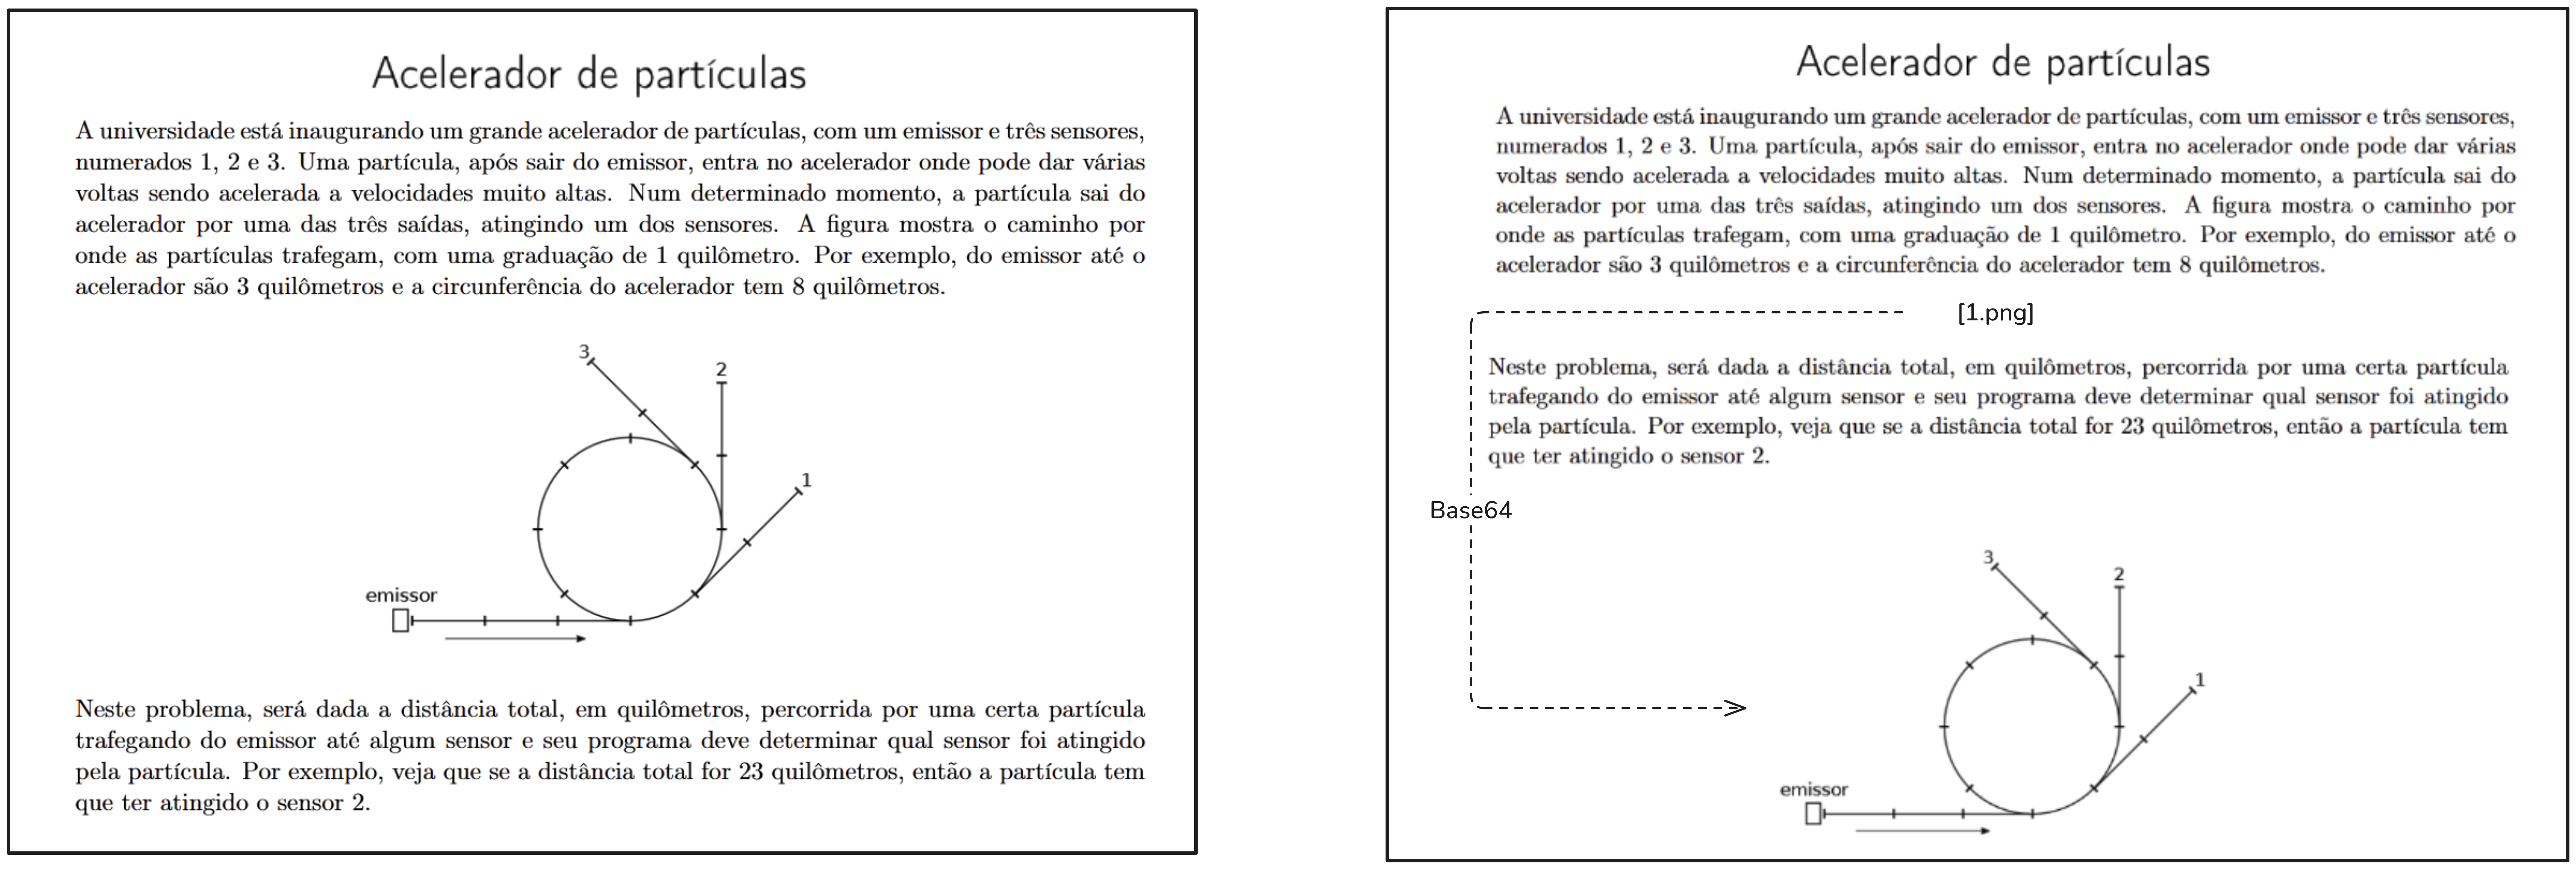
\includegraphics[width=\textwidth]{Cap04/figuras/enunciado-prompt-horizontal.png}
\caption[Representação de um enunciado com imagem no prompt]{Comparação entre o enunciado original da prova da OBI com figura (à esquerda) e a sua representação estruturada no \textit{prompt} com o marcador \texttt{[1.png]} associado à imagem codificada em Base64 (à direita).}
\label{fig:met-enunciado-prompt}
\end{figure}

\subsection{PP3: Explicitação de Limites de Tempo e Memória}\label{sec:met-rq3}

Para isolar o impacto da explicitação das restrições computacionais (\texttt{include\_limits=True}), seleciona-se a linguagem que apresentou a menor taxa agregada de aprovação na PP1 (\linguagem{C}), submetendo novamente todos os 125 problemas com os valores exatos de \texttt{time\_limit} e \texttt{memory\_limit} informados no \textit{prompt} (\promptname{zero\_shot.txt}).

\subsection{PP4: Estratégias de Engenharia de \texorpdfstring{\textit{Prompt}}{Prompt}}\label{sec:met-rq4}

Mantendo \linguagem{C} como linguagem-alvo de maior desafio no \textit{baseline}, comparam-se três estratégias de \textit{prompting} sobre os 125 problemas ($1.125$ execuções ao todo, cujos textos integrais constam do Apêndice~\ref{ap:prompts}): (i) \textit{Zero-Shot} (\promptname{zero\_shot.txt}); (ii) \textit{Few-Shot} (\promptname{few\_shot\_c.txt}), contendo três problemas canônicos em C voltados à prevenção de \textit{overflow}, E/S estrita e indexação 1-based; e (iii) \textit{Chain-of-Thought}~\citep{wei2022chain} guiado pela Metodologia de Pólya~\citep{polya1945} (\promptname{chain\_of\_thought\_polya.txt}), estruturado em Compreensão, Planejamento, Codificação (Execução) e Teste. Adicionalmente, conduz-se uma auditoria manual e programática (\textit{sanity check}) sobre os casos classificados como \veredito{CE} no \textit{CoT Pólya} para verificar se contêm código C compilável suprimido por artefatos de extração de múltiplos blocos Markdown (\textit{parser artifact}).

\subsection{PP5: Evolução Geracional sob Paridade de Juiz}\label{sec:met-rq5}

Para avaliar o progresso entre gerações consecutivas de LLMs sem introduzir distorções de protocolo, identificou-se a interseção exata entre a base Sênior deste TCC e o estudo preliminar do grupo~\citep{angelo2026ise,obibenchmarking2026}. Esse recorte corresponde à totalidade das \textbf{46 questões com figuras} do Nível Sênior da OBI (2016--2025), único subconjunto compartilhado que dispõe de execuções sob configuração idêntica em ambos os trabalhos: linguagem \linguagem{Python}, estratégia \textit{Zero-Shot}, modo texto puro (\modalidade{text}) e decodificação determinística ($T = 0{,}0$).

Uma etapa metodológica decisiva consistiu em \textbf{rejulgar localmente os códigos \texttt{.py} salvos da geração anterior} (\textbf{Gemini 3.1 Pro} e \textbf{GPT-5.4}) utilizando exatamente o mesmo \texttt{JudgeService} empregado para \textbf{Gemini 3.8 Flash} e \textbf{GPT-6 Luna}. No repositório anterior, o avaliador aplicava tempo limite fixo de $3{,}0\,\mathrm{s}$ para \linguagem{Python} (independentemente do limite oficial de $5{,}0\,\mathrm{s}$ previsto em diversas questões da OBI) e comparava saídas com remoção de espaços apenas nas extremidades da \textit{string} completa, em vez de linha a linha. Sem o rejulgamento no ambiente unificado (Python~3.14.3, limites oficiais por questão e monitoramento de memória via \texttt{psutil}), diferenças de infraestrutura seriam confundidas com ganhos ou perdas reais dos modelos.

Os resultados consolidados desse protocolo foram organizados no arquivo \href{https://github.com/mestrevh/competitive-programming-bench/blob/main/results/dataset_obi_senior/llms_compare.csv}{\texttt{results/dataset\_obi\_senior/llms\_compare.csv}}\footnote{Disponível em: \url{https://github.com/mestrevh/competitive-programming-bench/blob/main/results/dataset_obi_senior/llms_compare.csv}.}. Para preservar a simetria da análise pareada entre gerações, a avaliação na PP5 restringe-se às famílias com cobertura completa nos dois ciclos --- \textbf{Google} (\textit{Gemini 3.1 Pro} $\rightarrow$ \textit{Gemini 3.8 Flash}) e \textbf{OpenAI} (\textit{GPT-5.4} $\rightarrow$ \textit{GPT-6 Luna}). A família DeepSeek não entra nas tabelas e nos gráficos comparativos dessa seção porque o antecessor \textit{DeepSeek-V3.2} não possui execuções \linguagem{Python} \textit{Zero-Shot} no Nível Sênior, permanecendo registrado como \texttt{N/A} na base consolidada.

\section{Limitações}\label{sec:conc-limitacoes}

Embora o protocolo experimental tenha sido estruturado para garantir controle e reprodutibilidade, algumas limitações metodológicas devem ser consideradas. Primeiramente, a avaliação concentra-se na geração determinística ($T = 0{,}0$) com a métrica $\passat{1}$ (uma única submissão por problema e condição), diferindo de estudos que variam o parâmetro $k$ com temperaturas mais altas para explorar a diversidade amostral dos modelos.

Além disso, o escopo empírico principal restringe-se a três modelos atuais e às questões do Nível Sênior da OBI, enquanto a comparação geracional (PP5) limita-se à interseção de 46 questões com figuras em \linguagem{Python} \textit{Zero-Shot} e aos dois pares com cobertura completa (Google e OpenAI). Como os problemas correspondem a edições públicas aplicadas entre 2016 e 2025, não é possível descartar a hipótese de exposição prévia de parte dos enunciados ou soluções nos conjuntos de treinamento dos modelos. Por fim, o extrator automático de código apresenta sensibilidade a respostas que dividem a solução em múltiplos blocos Markdown, aspecto que motivou a auditoria específica de artefatos de extração na PP4.
\cleardoublepage

\chapter{Resultados e Discussão}\label{cap:resultados}

Este capítulo apresenta e discute os resultados empíricos obtidos na avaliação experimental do \textit{benchmark} da OBI Nível Sênior, organizados segundo a caracterização da base e as cinco perguntas de pesquisa definidas no Capítulo~\ref{cap:introducao}.

\section{Caracterização da Base e Validação Oráculo}\label{sec:res-base}

A base experimental consolidada (\texttt{dataset\_obi\_senior}) reúne \textbf{125 problemas} do Nível Sênior da OBI (2016 a 2025) e um total de \textbf{4.681 casos de teste} oficiais (média de $37{,}4$ casos por problema). Os limites computacionais definidos nos enunciados variam entre $1{,}0\,\mathrm{s}$ e $15{,}0\,\mathrm{s}$ para tempo de execução (com predomínio de $5{,}0\,\mathrm{s}$ em 59 questões e $1{,}0\,\mathrm{s}$ ou $2{,}0\,\mathrm{s}$ em 23 questões cada) e entre $256\,\mathrm{MB}$ (63 questões), $512\,\mathrm{MB}$ (44 questões) e $1.024\,\mathrm{MB}$ (18 questões) para memória.

A distribuição temporal das questões é apresentada na Figura~\ref{fig:res-base-ano}, destacando o pico de 20 problemas em 2020 e cobertura regular entre 10 e 17 questões nos demais anos analisados (exceto 2018, não incluído no recorte). Conforme mostra a Figura~\ref{fig:res-base-periodo}, a base apresenta equilíbrio entre as três etapas seletivas da competição: 43 questões na Fase~1 (incluindo Fase Local), 42 na Fase~2 (incluindo Fase Estadual e Turno~B) e 40 na Fase~3 (incluindo Fase Nacional). Quanto à composição visual (Figura~\ref{fig:res-base-imagens}), 79 enunciados ($63{,}2\%$) são puramente textuais e 46 ($36{,}8\%$) contêm ao menos uma imagem associada.

\begin{figure}[!htbp]
\centering
% Distribuição das 125 questões da OBI Nível Sênior por ano (Cap. 5, Seção 5.1)
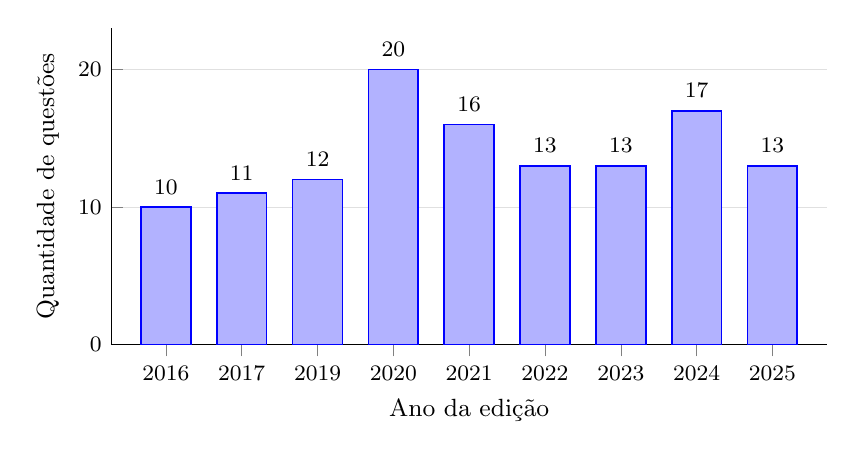
\begin{tikzpicture}
\begin{axis}[
  ybar,
  width=0.88\textwidth,
  height=5.6cm,
  bar width=18pt,
  ymin=0, ymax=23,
  ylabel={Quantidade de questões},
  xlabel={Ano da edição},
  symbolic x coords={2016,2017,2019,2020,2021,2022,2023,2024,2025},
  xtick=data,
  enlarge x limits=0.09,
  ymajorgrids=true,
  grid style={black!12},
  axis lines*=left,
  tick label style={font=\footnotesize},
  label style={font=\small},
  nodes near coords,
  nodes near coords style={font=\footnotesize\bfseries, black, yshift=1pt},
  every axis plot/.append style={fill=vAzul, draw=vAzul!70!black, line width=0.6pt}
]
\addplot coordinates {
  (2016,10) (2017,11) (2019,12) (2020,20) (2021,16) (2022,13) (2023,13) (2024,17) (2025,13)
};
\end{axis}
\end{tikzpicture}

\caption[Distribuição das questões da OBI Sênior por ano]{Distribuição das 125 questões do Nível Sênior da OBI por ano de edição (2016--2025).}
\label{fig:res-base-ano}
\end{figure}

\begin{figure}[!htbp]
\centering
% Distribuição das 125 questões da OBI Nível Sênior por fase (Cap. 5, Seção 5.1)
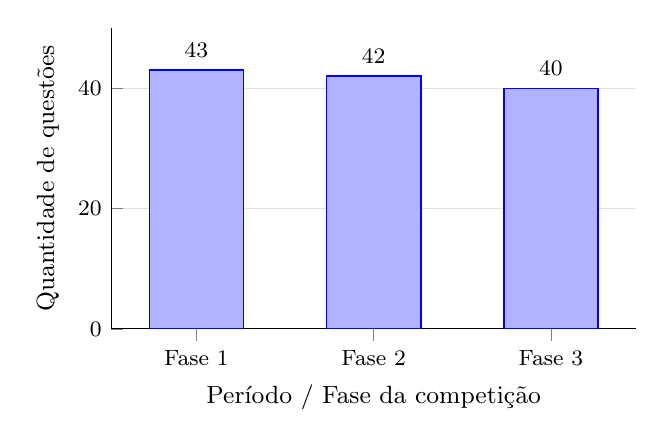
\begin{tikzpicture}
\begin{axis}[
  ybar,
  width=0.68\textwidth,
  height=5.4cm,
  bar width=34pt,
  ymin=0, ymax=50,
  ylabel={Quantidade de questões},
  xlabel={Período / Fase da competição},
  symbolic x coords={Fase 1,Fase 2,Fase 3},
  xtick=data,
  enlarge x limits=0.24,
  ymajorgrids=true,
  grid style={black!12},
  axis lines*=left,
  tick label style={font=\footnotesize},
  label style={font=\small},
  nodes near coords,
  nodes near coords style={font=\footnotesize\bfseries, black, yshift=1pt},
  every axis plot/.append style={fill=vAzul!85!vRoxo, draw=vAzul!65!black, line width=0.6pt}
]
\addplot coordinates {
  (Fase 1,43) (Fase 2,42) (Fase 3,40)
};
\end{axis}
\end{tikzpicture}

\caption[Distribuição das questões da OBI Sênior por período]{Distribuição das 125 questões do Nível Sênior da OBI por etapa da competição (Fases 1, 2 e 3).}
\label{fig:res-base-periodo}
\end{figure}

\begin{figure}[!htbp]
\centering
% Presença de imagens nos enunciados da OBI Nível Sênior (Cap. 5, Seção 5.1)
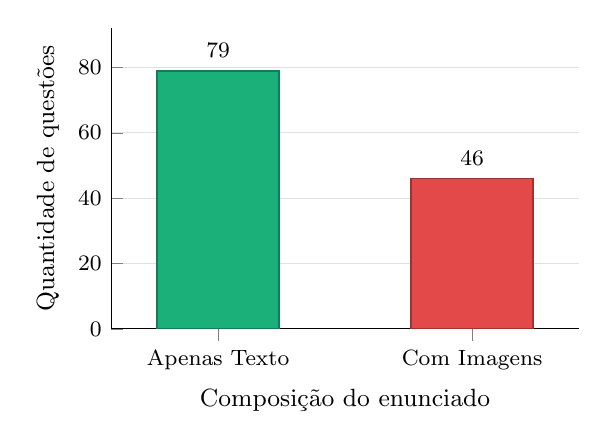
\begin{tikzpicture}
\begin{axis}[
  ybar,
  width=0.62\textwidth,
  height=5.4cm,
  bar width=44pt,
  ymin=0, ymax=92,
  ylabel={Quantidade de questões},
  xlabel={Composição do enunciado},
  symbolic x coords={Apenas Texto,Com Imagens},
  xtick={Apenas Texto,Com Imagens},
  enlarge x limits=0.42,
  ymajorgrids=true,
  grid style={black!12},
  axis lines*=left,
  tick label style={font=\footnotesize},
  label style={font=\small},
  nodes near coords,
  nodes near coords style={font=\footnotesize\bfseries, black, yshift=1pt}
]
\addplot[fill=vVerde, draw=vVerde!70!black, line width=0.6pt, bar shift=0pt] coordinates {
  (Apenas Texto,79)
};
\addplot[fill=vVermelho, draw=vVermelho!70!black, line width=0.6pt, bar shift=0pt] coordinates {
  (Com Imagens,46)
};
\end{axis}
\end{tikzpicture}

\caption[Distribuição das questões quanto à presença de imagens]{Proporção de questões com enunciado puramente textual versus questões com imagens associadas.}
\label{fig:res-base-imagens}
\end{figure}
\FloatBarrier

Na validação pelo modo oráculo, todas as \textbf{125 soluções de referência} obtiveram veredito \veredito{AC} ($100{,}0\%$ de aprovação), passando nos \textbf{4.681 casos de teste} oficiais sem nenhuma ocorrência de \veredito{WA}, \veredito{RE}, \veredito{TLE}, \veredito{MLE} ou \veredito{CE}. O tempo de execução observado nas soluções oráculo apresentou média de $0{,}254\,\mathrm{s}$, mediana de $0{,}180\,\mathrm{s}$ e máximo de $2{,}134\,\mathrm{s}$, confirmando a integridade do \textit{JudgeService} e dos gabaritos utilizados antes da avaliação dos LLMs. Os registros completos da execução oráculo encontram-se disponíveis em \href{https://github.com/mestrevh/competitive-programming-bench/blob/main/results/dataset_obi_senior/oracle.csv}{\texttt{oracle.csv}}\footnote{Disponível em: \url{https://github.com/mestrevh/competitive-programming-bench/blob/main/results/dataset_obi_senior/oracle.csv}.}.


\section{PP1: Desempenho Geral e Variação entre Linguagens}\label{sec:res-rq1}

Para manter um \textit{baseline} nas próximas perguntas, a primeira pergunta é importante para entender qual é o impacto dos diferentes tipos de linguagens, buscando realizar de forma simples a criação das soluções dos problemas em relação às linguagens. Nas cinco baterias de testes, utiliza-se apenas texto com a técnica \promptname{zero\_shot.txt} (Apêndice~\ref{ap:prompts}) para as 125 questões do Nível Sênior da OBI, Modalidade Programação, e os modelos utilizados foram: \textbf{DeepSeek v4.1 Flash}, \textbf{Gemini 3.8 Flash} e \textbf{GPT-6 Luna}.

Observando as linguagens, quando se verifica a característica de serem fracamente tipadas, como \linguagem{Python} e \linguagem{JavaScript}, os modelos não precisam se preocupar com a tipagem para as variáveis do problema; porém, isso é ruim para a programação competitiva devido à abordagem desse tipo de prova em relação aos limites de variáveis, trazendo mais decisões para a produção de uma solução \veredito{AC}. Por isso, a linguagem \linguagem{Python} teve destaque apenas no modelo \textbf{Gemini 3.8 Flash}, com 121 acertos (no agregado, 92,80\%), como mostra a Figura~\ref{fig:res-pp1-ac-linguagem}.

\begin{figure}[!htbp]
\centering
% Gráfico de barras agrupadas: quantidade de AC por LLM e Linguagem + Agregado (Cap. 5, Seção 5.2)
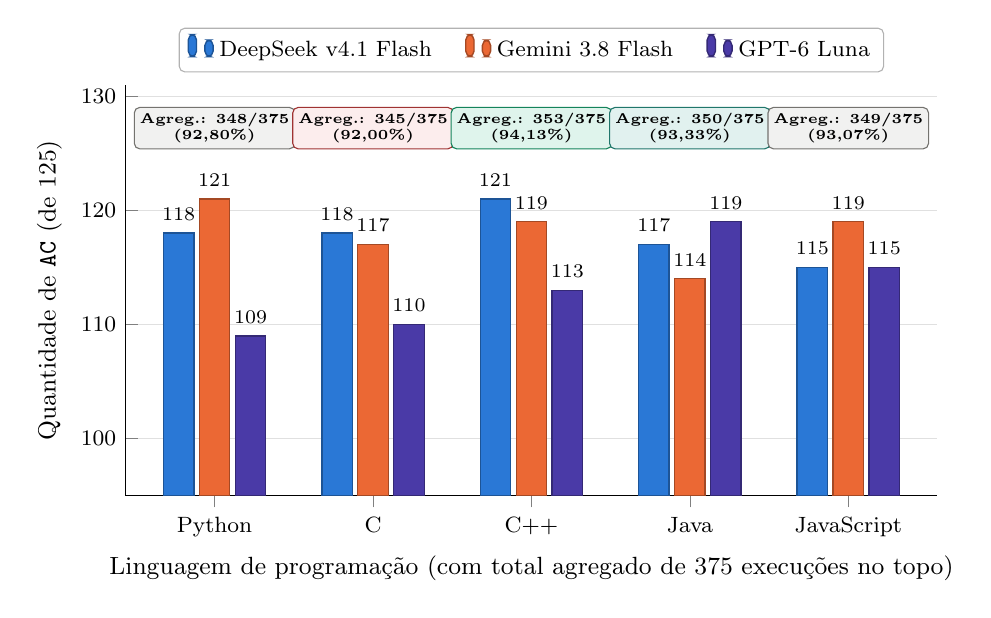
\begin{tikzpicture}
\begin{axis}[
  ybar=2pt,
  width=0.98\textwidth,
  height=6.8cm,
  bar width=11pt,
  ymin=95, ymax=131,
  ylabel={Quantidade de \veredito{AC} (de 125)},
  xlabel={Linguagem de programação (com total agregado de 375 execuções no topo)},
  symbolic x coords={Python,C,C++,Java,JavaScript},
  xtick=data,
  enlarge x limits=0.14,
  ymajorgrids=true,
  grid style={black!12},
  axis lines*=left,
  tick label style={font=\footnotesize},
  label style={font=\small},
  legend style={
    at={(0.5,1.03)},
    anchor=south,
    legend columns=3,
    draw=black!30,
    rounded corners=2pt,
    font=\footnotesize,
    /tikz/every even column/.append style={column sep=10pt}
  },
  nodes near coords,
  nodes near coords style={font=\scriptsize\bfseries, black, yshift=1pt}
]
\addplot[fill=vAzul, draw=vAzul!70!black, line width=0.5pt] coordinates {
  (Python,118) (C,118) (C++,121) (Java,117) (JavaScript,115)
};
\addplot[fill=vLaranja, draw=vLaranja!70!black, line width=0.5pt] coordinates {
  (Python,121) (C,117) (C++,119) (Java,114) (JavaScript,119)
};
\addplot[fill=vRoxo, draw=vRoxo!70!black, line width=0.5pt] coordinates {
  (Python,109) (C,110) (C++,113) (Java,119) (JavaScript,115)
};
\legend{DeepSeek v4.1 Flash, Gemini 3.8 Flash, GPT-6 Luna}

% Pílulas com o Agregado Total da Tabela 5.1 (de 375 execuções por linguagem)
\node[font=\tiny\bfseries, align=center, fill=vCinza!14, draw=vCinza!75!black, rounded corners=2pt, inner sep=2pt]
  at (axis cs:Python,127.2) {Agreg.: 348/375\\(92,80\%)};
\node[font=\tiny\bfseries, align=center, fill=vVermelho!10, draw=vVermelho!70!black, rounded corners=2pt, inner sep=2pt]
  at (axis cs:C,127.2) {Agreg.: 345/375\\(92,00\%)};
\node[font=\tiny\bfseries, align=center, fill=vVerde!14, draw=vVerde!75!black, rounded corners=2pt, inner sep=2pt]
  at (axis cs:C++,127.2) {Agreg.: 353/375\\(94,13\%)};
\node[font=\tiny\bfseries, align=center, fill=vTeal!14, draw=vTeal!75!black, rounded corners=2pt, inner sep=2pt]
  at (axis cs:Java,127.2) {Agreg.: 350/375\\(93,33\%)};
\node[font=\tiny\bfseries, align=center, fill=vCinza!14, draw=vCinza!75!black, rounded corners=2pt, inner sep=2pt]
  at (axis cs:JavaScript,127.2) {Agreg.: 349/375\\(93,07\%)};
\end{axis}
\end{tikzpicture}

\caption[Quantidade de submissões aceitas por LLM, linguagem e total agregado na PP1]{Quantidade de submissões aprovadas (\veredito{AC} de 125) por modelo e linguagem de programação na linha de base ($T = 0{,}0$), acompanhada do total agregado (de 375 execuções por linguagem).}
\label{fig:res-pp1-ac-linguagem}
\end{figure}
\FloatBarrier

Em contrapartida, as linguagens fortemente tipadas \linguagem{C}, \linguagem{C++} e \linguagem{Java} tiveram desempenhos distintos. Para o modelo \textbf{GPT-6 Luna}, a linguagem que performou melhor foi \linguagem{Java}, com 119 acertos (no agregado, 93,33\%), já para o \textbf{DeepSeek v4.1 Flash} a melhor linguagem foi \linguagem{C++}. Na comunidade de programação competitiva, geralmente a linguagem utilizada é \linguagem{C++}, o que se destaca pelo fato de ela ter obtido o melhor desempenho no agregado, com 94,13\%. Por isso, \linguagem{C++} pode ser a linguagem com uma exposição maior aos dados durante o treinamento dos modelos.

\begin{table}[!htbp]
\centering
\caption[Estabilidade entre linguagens na PP1]{Média de acerto ($\passat{1}$), desvio padrão ($\sigma$) e amplitude entre as cinco linguagens avaliadas sobre as 125 questões da OBI Sênior.}
\label{tab:res-pp1-estabilidade}
\small
\begin{tabular}{lccc}
\toprule
Modelo & Média $\passat{1}$ & Desvio Padrão ($\sigma$) & Amplitude (Máx--Mín) \\
\midrule
DeepSeek v4.1 Flash & 94,24\% & \tfirst{1,55 p.p.}  & \tfirst{4,80 p.p.} \\
Gemini 3.8 Flash    & \tfirst{94,40\%} & \tsecond{1,89 p.p.} & \tsecond{5,60 p.p.} \\
GPT-6 Luna          & 90,56\% & 2,88 p.p.           & 8,00 p.p. \\
\bottomrule
\end{tabular}
\end{table}

Ao verificar a distribuição em relação a todas as linguagens (Tabela~\ref{tab:res-pp1-estabilidade}), observa-se uma taxa média de acerto ($\passat{1}$) elevada nos três modelos --- com 94,40\% no \textbf{Gemini 3.8 Flash}, 94,24\% no \textbf{DeepSeek v4.1 Flash} e 90,56\% no \textbf{GPT-6 Luna} ---, sendo que o \textbf{DeepSeek v4.1 Flash} foi o que teve o melhor desempenho de estabilidade, com o menor desvio e, consequentemente, com a menor amplitude. Por isso, quando se busca \textit{performance}, é recomendável utilizar esse modelo para a configuração com temperatura zero, buscando menor variação em soluções com linguagens diferentes.

Entretanto, observando as tomadas de decisões para a criação da solução, o modelo \textbf{GPT-6 Luna} foi o que teve menor desempenho, demonstrando que o modelo é sensível aos diferentes tipos de linguagens. Isso é importante em relação às tomadas de decisões durante a construção da solução \textit{token} a \textit{token}. Pois, durante a criação da solução, é necessário tomar decisões sintáticas e semânticas para cada linguagem e, mesmo com modelos mais sofisticados, mostra-se que nem sempre o domínio do problema é garantia para a construção de uma solução executável.

\begin{table}[!htbp]
\centering
\caption[Resumo agregado de vereditos por linguagem na PP1]{Distribuição agregada de falhas e aprovações por linguagem (375 execuções por linguagem).}
\label{tab:res-pp1-erros-lang}
\small
\begin{tabular}{lccccccc}
\toprule
Linguagem & \veredito{WA} & \veredito{CE} & \veredito{RE} & \veredito{TLE} & \veredito{MLE} & Total Erros & \veredito{AC} ($\passat{1}$) \\
\midrule
Python     & 21 & 2  & 1 & 3 & 0 & 27 & 348 (92,80\%) \\
C          & 17 & 13 & 0 & 0 & 0 & 30 & 345 (92,00\%) \\
C++        & 19 & 2  & 0 & 1 & 0 & 22 & 353 (94,13\%) \\
Java       & 17 & 3  & 4 & 0 & 1 & 25 & 350 (93,33\%) \\
JavaScript & 20 & 2  & 2 & 0 & 2 & 26 & 349 (93,07\%) \\
\bottomrule
\end{tabular}
\end{table}

Ao observar a Tabela~\ref{tab:res-pp1-erros-lang}, o destaque está na linguagem \linguagem{C}: por ser bastante manual a criação da solução, os modelos precisam tomar bastantes decisões, pois devem criar as estruturas de dados, preocupar-se com a tipagem das variáveis, pilha de execução, etc. Por isso, quanto maior o código final, maior é a probabilidade de existirem ruídos que causam tanto erro de compilação (\veredito{CE}) quanto resposta errada (\veredito{WA}).

\begin{figure}[!htbp]
\centering
% Gráficos lado a lado: LOC médio e Tempo Médio de CPU em soluções AC (Cap. 5, Seção 5.2.3)
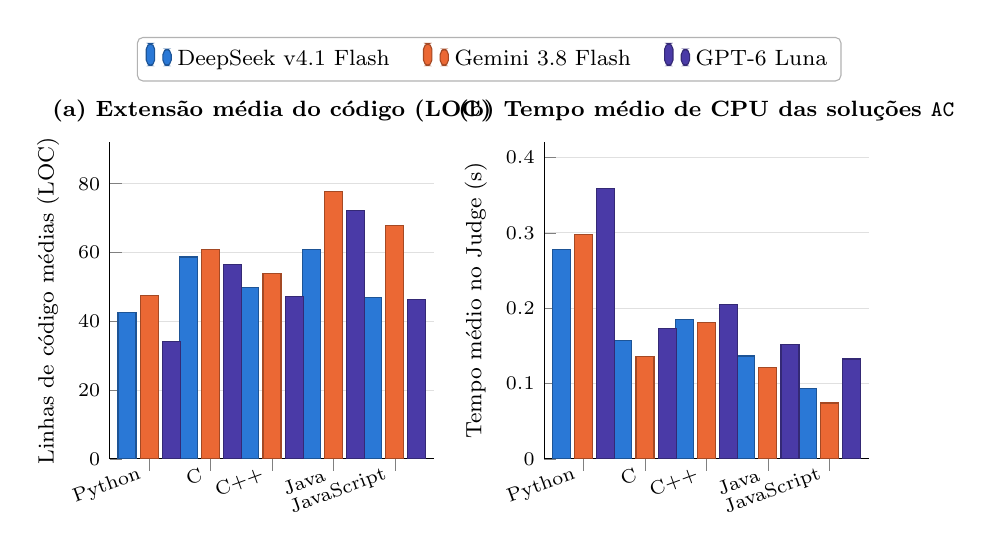
\begin{tikzpicture}
\begin{groupplot}[
  group style={
    group size=2 by 1,
    horizontal sep=1.4cm
  },
  width=0.47\textwidth,
  height=5.6cm,
  symbolic x coords={Python,C,C++,Java,JavaScript},
  xtick=data,
  enlarge x limits=0.16,
  ymajorgrids=true,
  grid style={black!12},
  axis lines*=left,
  tick label style={font=\scriptsize},
  x tick label style={rotate=20, anchor=east},
  label style={font=\footnotesize},
  title style={font=\footnotesize\bfseries, yshift=-2pt}
]
% Painel (a): LOC médio
\nextgroupplot[
  ybar=1.5pt,
  bar width=6.5pt,
  title={(a) Extensão média do código (LOC)},
  ymin=0, ymax=92,
  ylabel={Linhas de código médias (LOC)},
  legend to name=legpp1loctempo,
  legend style={
    legend columns=3,
    draw=black!30,
    rounded corners=2pt,
    font=\footnotesize,
    /tikz/every even column/.append style={column sep=10pt}
  }
]
\addplot[fill=vAzul, draw=vAzul!70!black, line width=0.4pt] coordinates {
  (Python,42.6) (C,58.7) (C++,49.9) (Java,60.8) (JavaScript,46.8)
};
\addplot[fill=vLaranja, draw=vLaranja!70!black, line width=0.4pt] coordinates {
  (Python,47.6) (C,60.9) (C++,53.9) (Java,77.7) (JavaScript,67.9)
};
\addplot[fill=vRoxo, draw=vRoxo!70!black, line width=0.4pt] coordinates {
  (Python,34.2) (C,56.4) (C++,47.3) (Java,72.3) (JavaScript,46.4)
};
\legend{DeepSeek v4.1 Flash, Gemini 3.8 Flash, GPT-6 Luna}

% Painel (b): Tempo médio de CPU (AC)
\nextgroupplot[
  ybar=1.5pt,
  bar width=6.5pt,
  title={(b) Tempo médio de CPU das soluções \veredito{AC}},
  ymin=0, ymax=0.42,
  ylabel={Tempo médio no Judge (s)}
]
\addplot[fill=vAzul, draw=vAzul!70!black, line width=0.4pt] coordinates {
  (Python,0.2776) (C,0.1569) (C++,0.1856) (Java,0.1365) (JavaScript,0.0929)
};
\addplot[fill=vLaranja, draw=vLaranja!70!black, line width=0.4pt] coordinates {
  (Python,0.2973) (C,0.1360) (C++,0.1811) (Java,0.1213) (JavaScript,0.0742)
};
\addplot[fill=vRoxo, draw=vRoxo!70!black, line width=0.4pt] coordinates {
  (Python,0.3595) (C,0.1734) (C++,0.2048) (Java,0.1517) (JavaScript,0.1326)
};
\end{groupplot}

% Legenda compartilhada acima dos dois gráficos
\node[anchor=south] at ($(group c1r1.north)!0.5!(group c2r1.north) + (0,0.65cm)$)
  {\pgfplotslegendfromname{legpp1loctempo}};
\end{tikzpicture}

\caption[Extensão média do código e tempo médio de CPU na PP1]{Comparativo por modelo e linguagem quanto (a) ao número médio de linhas de código (LOC) e (b) ao tempo médio de execução em CPU das soluções aprovadas (\veredito{AC}).}
\label{fig:res-pp1-loc-tempo}
\end{figure}
\FloatBarrier

Entretanto, ao verificar a produção média de linhas por código na Figura~\ref{fig:res-pp1-loc-tempo}, que está estritamente ligada à predição dos \textit{tokens} e à construção da solução executável, nota-se que \linguagem{C} não é a linguagem com o maior número de linhas (e nem de \textit{tokens}). Por consequência, esses erros estão concentrados principalmente na semântica ou na sintaxe da projeção da resolução do problema. Em \linguagem{Java} e \linguagem{C++} existem bibliotecas com estruturas de dados e funções, entre outros recursos, que ajudam na construção do raciocínio do problema.

Em paralelo, verificando o desempenho em relação ao tempo de execução de CPU, a linguagem \linguagem{Python} teve o pior desempenho nos três modelos. Pensando em \textit{performance}, é recomendável utilizar o \textbf{Gemini 3.8 Flash}, pois teve o melhor desempenho em relação aos outros LLMs. Para mais informações sobre gasto de \textit{tokens}, custo, etc., verifique o Apêndice~\ref{ap:resultados-complementares} (Seção~\ref{ap:pp1-detalhes}).

Por fim, como \textit{baseline} para as próximas perguntas, a linguagem \linguagem{C++} será utilizada no teste com imagens por ter o melhor desempenho geral (94,13\% no agregado), e a linguagem \linguagem{C}, por ter registrado a menor taxa de acerto (92,00\% no agregado), será principalmente utilizada nos testes em que o \textit{prompt} informa o tempo de execução e a memória do problema, bem como no teste com técnicas de \textit{prompt}.


\section{PP2: Impacto das Imagens e Modalidades Multimodais}\label{sec:res-rq2}

A base de dados utilizada para este estudo possui 46 questões com imagens. Ao construir o \textit{baseline} com a estratégia \promptname{zero\_shot} e sabendo que a linguagem \linguagem{C++} foi a que melhor performou, verificou-se, nesse subconjunto de questões, que a presença de figuras reduz a taxa de acerto de todos os modelos quando avaliados apenas por texto em comparação às 79 questões sem imagens (Tabela~\ref{tab:res-pp2-baseline} do Apêndice~\ref{ap:resultados-complementares}), mostrando que as imagens impactam diretamente na solução proposta pelos modelos e, consequentemente, no veredito do \textit{Judge}. Por isso, as novas baterias de testes foram feitas com as imagens no formato Base64 (\modalidade{img}), sendo referenciadas no enunciado conforme mencionado na Metodologia (Figura~\ref{fig:met-enunciado-prompt}). Além disso, existe um campo no JSON do problema que contém a descrição textual de cada figura (\modalidade{description}), o qual é colocado diretamente no lugar da imagem.

\begin{figure}[!htbp]
\centering
% Gráfico de barras agrupadas: Pass@1 em C++ nas três modalidades (Cap. 5, Seção 5.3.2)
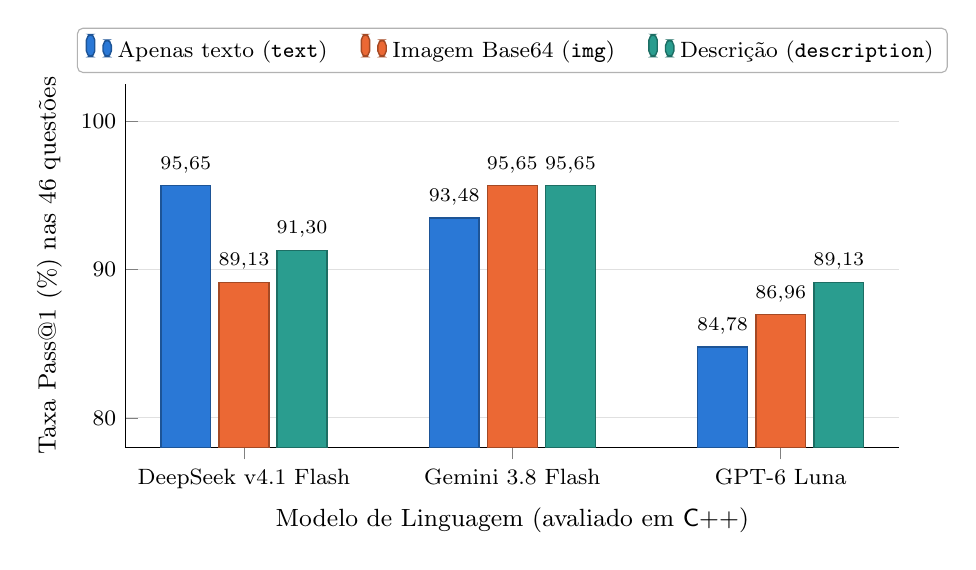
\begin{tikzpicture}
\begin{axis}[
  ybar=3pt,
  width=0.94\textwidth,
  height=6.2cm,
  bar width=18pt,
  ymin=78, ymax=102.5,
  ylabel={Taxa \passat{1} (\%) nas 46 questões},
  xlabel={Modelo de Linguagem (avaliado em \linguagem{C++})},
  symbolic x coords={DeepSeek v4.1 Flash,Gemini 3.8 Flash,GPT-6 Luna},
  xtick={DeepSeek v4.1 Flash,Gemini 3.8 Flash,GPT-6 Luna},
  enlarge x limits=0.22,
  ymajorgrids=true,
  grid style={black!12},
  axis lines*=left,
  tick label style={font=\footnotesize},
  label style={font=\small},
  legend style={
    at={(0.5,1.03)},
    anchor=south,
    legend columns=3,
    draw=black!30,
    rounded corners=2pt,
    font=\footnotesize,
    /tikz/every even column/.append style={column sep=10pt}
  },
  nodes near coords,
  nodes near coords style={
    font=\scriptsize\bfseries,
    black,
    yshift=1pt,
    /pgf/number format/fixed,
    /pgf/number format/fixed zerofill,
    /pgf/number format/precision=2,
    /pgf/number format/use comma
  }
]
\addplot[fill=vAzul, draw=vAzul!70!black, line width=0.5pt] coordinates {
  (DeepSeek v4.1 Flash,95.65) (Gemini 3.8 Flash,93.48) (GPT-6 Luna,84.78)
};
\addplot[fill=vLaranja, draw=vLaranja!70!black, line width=0.5pt] coordinates {
  (DeepSeek v4.1 Flash,89.13) (Gemini 3.8 Flash,95.65) (GPT-6 Luna,86.96)
};
\addplot[fill=vTeal, draw=vTeal!70!black, line width=0.5pt] coordinates {
  (DeepSeek v4.1 Flash,91.30) (Gemini 3.8 Flash,95.65) (GPT-6 Luna,89.13)
};
\legend{Apenas texto (\texttt{text}), Imagem Base64 (\texttt{img}), Descrição (\texttt{description})}
\end{axis}
\end{tikzpicture}

\caption[Pass@1 em C++ nas três modalidades da PP2]{Comparação da taxa \passat{1} em \linguagem{C++} sobre as $46$ questões com figuras nas modalidades \modalidade{text}, \modalidade{img} (Base64) e \modalidade{description}.}
\label{fig:res-pp2-modalidades}
\end{figure}
\FloatBarrier

Ao analisar a Figura~\ref{fig:res-pp2-modalidades}, por meio da taxa $\passat{1}$ na linguagem \linguagem{C++}, vê-se que no modelo \textbf{DeepSeek v4.1 Flash} houve uma degradação acentuada ao utilizar imagens ou ao aumentar a base de informações dentro do \textit{prompt}. Isso mostra que esse modelo ainda não responde bem à construção de \textit{prompts} multimodais, diferentemente dos outros dois modelos. Porém, o que mais se destaca é que, utilizando o texto que descreve as imagens (\modalidade{description}), os modelos tiveram uma melhora significativa em relação à utilização direta da imagem (\modalidade{img}). Devido a isso, a construção da solução por meio de \textit{prompt} textual continua sendo a melhor forma de performar nesse \textit{dataset} de questões do Nível Sênior da OBI.

\begin{table}[!htbp]
\centering
\caption[Comparativo controlado em C++ nas 46 questões com imagens por modalidade]{Comparativo controlado em \linguagem{C++} nas $46$ questões com imagens por modalidade (PP2).}
\label{tab:res-pp2-modalidades}
\small
\begin{tabular}{@{}llccccccc@{}}
\toprule
\textbf{LLM} & \textbf{Modalidade} & \textbf{AC} & \textbf{Taxa \passat{1}} & \textbf{WA} & \textbf{RE} & \textbf{TLE} & \textbf{MLE} & \textbf{CE} \\
\midrule
DeepSeek v4.1 Flash & \modalidade{text}        & \tfirst{44}  & \tfirst{95,65\%}  & $1$ & $0$ & $0$ & $0$ & $1$ \\
DeepSeek v4.1 Flash & \modalidade{img}         & $41$         & $89{,}13\%$       & $2$ & $0$ & $0$ & $0$ & $3$ \\
DeepSeek v4.1 Flash & \modalidade{description} & \tsecond{42} & \tsecond{91,30\%} & $4$ & $0$ & $0$ & $0$ & $0$ \\
\midrule
Gemini 3.8 Flash    & \modalidade{text}        & $43$         & $93{,}48\%$       & $3$ & $0$ & $0$ & $0$ & $0$ \\
Gemini 3.8 Flash    & \modalidade{img}         & \tfirst{44}  & \tfirst{95,65\%}  & $2$ & $0$ & $0$ & $0$ & $0$ \\
Gemini 3.8 Flash    & \modalidade{description} & \tfirst{44}  & \tfirst{95,65\%}  & $2$ & $0$ & $0$ & $0$ & $0$ \\
\midrule
GPT-6 Luna          & \modalidade{text}        & $39$         & $84{,}78\%$       & $6$ & $0$ & $0$ & $0$ & $1$ \\
GPT-6 Luna          & \modalidade{img}         & \tsecond{40} & \tsecond{86,96\%} & $6$ & $0$ & $0$ & $0$ & $0$ \\
GPT-6 Luna          & \modalidade{description} & \tfirst{41}  & \tfirst{89,13\%}  & $5$ & $0$ & $0$ & $0$ & $0$ \\
\bottomrule
\end{tabular}
\end{table}

Como é visível na Tabela~\ref{tab:res-pp2-modalidades}, o teste com a descrição da imagem (\modalidade{description}) foi o único que não produziu códigos com erro de compilação (\veredito{CE}). Então, a predição para a criação de um código executável para esses modelos deve seguir o padrão textual, visto que o cálculo vetorial para o LLM conseguir processar imagem e texto impacta diretamente no cálculo da predição e, consequentemente, no código produzido como resposta.

\begin{figure}[!htbp]
\centering
% Gráficos lado a lado: Tokens médios de entrada e Custo Total USD (Cap. 5, Seção 5.3.3)
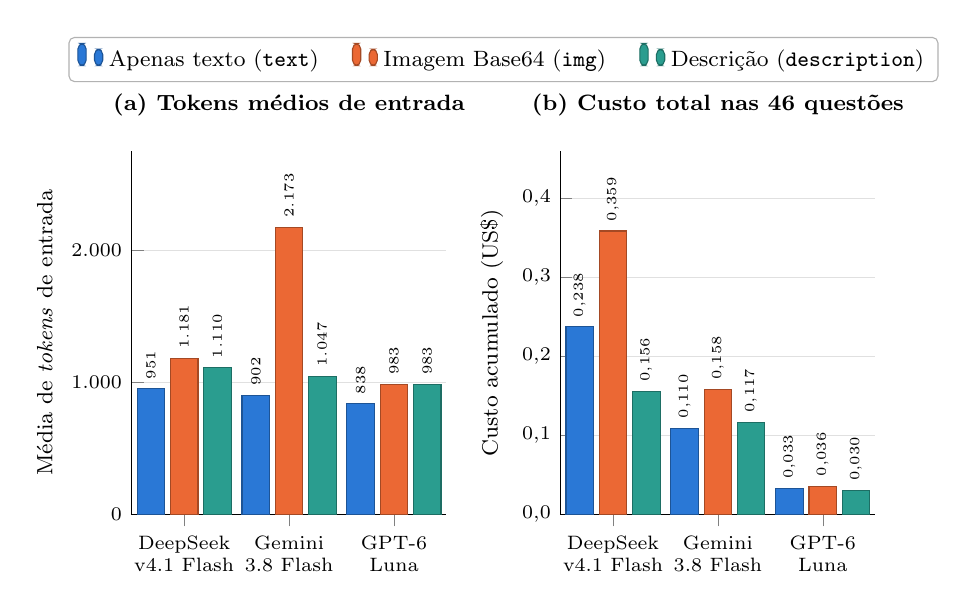
\begin{tikzpicture}
\begin{groupplot}[
  group style={
    group size=2 by 1,
    horizontal sep=1.45cm
  },
  width=0.46\textwidth,
  height=6.2cm,
  symbolic x coords={DeepSeek,Gemini,GPT6},
  xtick={DeepSeek,Gemini,GPT6},
  xticklabels={DeepSeek\\v4.1 Flash,Gemini\\3.8 Flash,GPT-6\\Luna},
  x tick label style={align=center},
  enlarge x limits=0.25,
  ymajorgrids=true,
  grid style={black!12},
  axis lines*=left,
  tick label style={font=\scriptsize},
  label style={font=\footnotesize},
  title style={font=\footnotesize\bfseries, yshift=3pt}
]
% Painel (a): Tokens médios de entrada
\nextgroupplot[
  ybar=2pt,
  bar width=10pt,
  title={(a) Tokens médios de entrada},
  ymin=0, ymax=2750,
  ylabel={Média de \textit{tokens} de entrada},
  yticklabel style={/pgf/number format/fixed, /pgf/number format/1000 sep={.}},
  legend to name=legpp2tokenscusto,
  legend style={
    legend columns=3,
    draw=black!30,
    rounded corners=2pt,
    font=\footnotesize,
    /tikz/every even column/.append style={column sep=10pt}
  },
  nodes near coords,
  nodes near coords style={
    font=\tiny\bfseries,
    black,
    rotate=90,
    anchor=west,
    /pgf/number format/fixed,
    /pgf/number format/precision=0,
    /pgf/number format/1000 sep={.}
  }
]
\addplot[fill=vAzul, draw=vAzul!70!black, line width=0.4pt] coordinates {
  (DeepSeek,950.8) (Gemini,901.5) (GPT6,838.2)
};
\addplot[fill=vLaranja, draw=vLaranja!70!black, line width=0.4pt] coordinates {
  (DeepSeek,1181.3) (Gemini,2173.1) (GPT6,983.0)
};
\addplot[fill=vTeal, draw=vTeal!70!black, line width=0.4pt] coordinates {
  (DeepSeek,1110.0) (Gemini,1046.6) (GPT6,982.6)
};
\legend{Apenas texto (\texttt{text}), Imagem Base64 (\texttt{img}), Descrição (\texttt{description})}

% Painel (b): Custo total (USD) nas 46 questões
\nextgroupplot[
  ybar=2pt,
  bar width=10pt,
  title={(b) Custo total nas 46 questões},
  ymin=0, ymax=0.46,
  ytick={0,0.1,0.2,0.3,0.4},
  ylabel={Custo acumulado (US\$)},
  yticklabel style={/pgf/number format/fixed, /pgf/number format/fixed zerofill, /pgf/number format/precision=1, /pgf/number format/use comma},
  nodes near coords,
  nodes near coords style={
    font=\tiny\bfseries,
    black,
    rotate=90,
    anchor=west,
    /pgf/number format/fixed,
    /pgf/number format/fixed zerofill,
    /pgf/number format/precision=3,
    /pgf/number format/use comma
  }
]
\addplot[fill=vAzul, draw=vAzul!70!black, line width=0.4pt] coordinates {
  (DeepSeek,0.2375) (Gemini,0.1095) (GPT6,0.0328)
};
\addplot[fill=vLaranja, draw=vLaranja!70!black, line width=0.4pt] coordinates {
  (DeepSeek,0.3588) (Gemini,0.1582) (GPT6,0.0360)
};
\addplot[fill=vTeal, draw=vTeal!70!black, line width=0.4pt] coordinates {
  (DeepSeek,0.1558) (Gemini,0.1166) (GPT6,0.0304)
};
\end{groupplot}

% Legenda compartilhada acima dos dois gráficos
\node[anchor=south] at ($(group c1r1.north)!0.5!(group c2r1.north) + (0,0.75cm)$)
  {\pgfplotslegendfromname{legpp2tokenscusto}};
\end{tikzpicture}

\caption[Tokens de entrada e custo total por modalidade na PP2]{Telemetria das $46$ questões em \linguagem{C++} por modalidade: (a) média de \textit{tokens} de entrada por problema e (b) custo financeiro total em dólares.}
\label{fig:res-pp2-tokens-custo}
\end{figure}
\FloatBarrier

Esse cálculo é refletido nos \textit{tokens} de entrada (\textit{prompt}): vê-se que todos os testes que utilizam imagem têm um valor alto, destacando-se o \textbf{Gemini 3.8 Flash}; em sequência, isso se refletiu no custo total, sendo que a bateria de testes com imagens (\modalidade{img}) foi a que teve o maior custo entre todas, como mostra a Figura~\ref{fig:res-pp2-tokens-custo}.

Contudo, houve uma questão na qual, mesmo com todos os testes realizados até agora, os modelos não obtiveram sucesso: o problema \textit{Construção de Rodovia} mostra que a validação literal que o \textit{Judge} possui faz com que a ordem importe durante a construção da solução. Essa é uma das habilidades que um competidor precisa possuir para reconhecer quando esse tipo de entrada e saída deve ser tratado. Assim, no Apêndice~\ref{ap:resultados-complementares} (Seção~\ref{ap:pp2-detalhes}) encontram-se a Tabela~\ref{tab:res-pp2-divergencias}, com as 15 questões em que houve divergências durante essas baterias de testes da PP2, e as demais análises complementares.

\section{PP3: Impacto das Restrições de Tempo e Memória em C}\label{sec:res-rq3}

Com base no \textit{baseline} estabelecido na PP1, a linguagem que registrou a menor taxa de aprovação no $\passat{1}$ foi a linguagem \linguagem{C}, com 92,00\% de acerto. Conforme discutido na Seção~\ref{sec:res-rq1}, para criar uma solução nessa linguagem é necessário realizar a construção manual de estruturas de dados e a manipulação de ponteiros, entre outros aspectos. Assim, esta etapa (PP3) busca verificar se o direcionamento explícito informando a quantidade limite de memória (\texttt{memory\_limit}) e de tempo (\texttt{time\_limit}) consegue proporcionar um direcionamento melhor sobre a construção do código executável. Além disso, o teste foi submetido conforme o protocolo da PP1 (temperatura $T = 0{,}0$ e técnica de \textit{prompt} \promptname{zero\_shot.txt}) para a linguagem \linguagem{C}.

\begin{figure}[!htbp]
\centering
% Gráfico comparativo: Pass@1 (%) em C no Baseline vs PP3 Com Limites (Cap. 5, Seção 5.4.1)
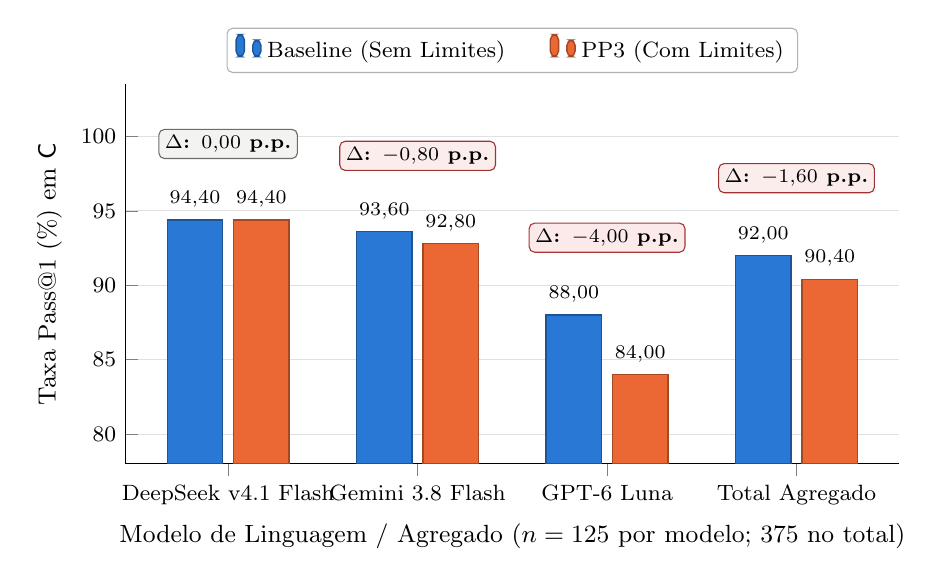
\begin{tikzpicture}
\begin{axis}[
  ybar=4pt,
  width=0.94\textwidth,
  height=6.4cm,
  bar width=20pt,
  ymin=78, ymax=103.5,
  ytick={80,85,90,95,100},
  ylabel={Taxa \passat{1} (\%) em \linguagem{C}},
  xlabel={Modelo de Linguagem / Agregado ($n=125$ por modelo; $375$ no total)},
  symbolic x coords={DeepSeek v4.1 Flash,Gemini 3.8 Flash,GPT-6 Luna,Total Agregado},
  xtick={DeepSeek v4.1 Flash,Gemini 3.8 Flash,GPT-6 Luna,Total Agregado},
  enlarge x limits=0.18,
  ymajorgrids=true,
  grid style={black!12},
  axis lines*=left,
  tick label style={font=\footnotesize},
  label style={font=\small},
  legend style={
    at={(0.5,1.03)},
    anchor=south,
    legend columns=2,
    draw=black!30,
    rounded corners=2pt,
    font=\footnotesize,
    /tikz/every even column/.append style={column sep=14pt}
  },
  nodes near coords,
  nodes near coords style={
    font=\scriptsize\bfseries,
    black,
    yshift=1pt,
    /pgf/number format/fixed,
    /pgf/number format/fixed zerofill,
    /pgf/number format/precision=2,
    /pgf/number format/use comma
  }
]
\addplot[fill=vAzul, draw=vAzul!70!black, line width=0.5pt] coordinates {
  (DeepSeek v4.1 Flash,94.40) (Gemini 3.8 Flash,93.60) (GPT-6 Luna,88.00) (Total Agregado,92.00)
};
\addplot[fill=vLaranja, draw=vLaranja!70!black, line width=0.5pt] coordinates {
  (DeepSeek v4.1 Flash,94.40) (Gemini 3.8 Flash,92.80) (GPT-6 Luna,84.00) (Total Agregado,90.40)
};
\legend{Baseline (Sem Limites), PP3 (Com Limites)}

% Pílulas com a variação (Delta) acima de cada par
\node[font=\scriptsize\bfseries, fill=vCinza!12, draw=vCinza!70!black, rounded corners=2pt, inner sep=2.2pt]
  at (axis cs:DeepSeek v4.1 Flash,99.5) {$\Delta$: $0{,}00$ p.p.};
\node[font=\scriptsize\bfseries, fill=vVermelho!10, draw=vVermelho!70!black, rounded corners=2pt, inner sep=2.2pt]
  at (axis cs:Gemini 3.8 Flash,98.7) {$\Delta$: $-0{,}80$ p.p.};
\node[font=\scriptsize\bfseries, fill=vVermelho!12, draw=vVermelho!75!black, rounded corners=2pt, inner sep=2.2pt]
  at (axis cs:GPT-6 Luna,93.2) {$\Delta$: $-4{,}00$ p.p.};
\node[font=\scriptsize\bfseries, fill=vVermelho!10, draw=vVermelho!70!black, rounded corners=2pt, inner sep=2.2pt]
  at (axis cs:Total Agregado,97.2) {$\Delta$: $-1{,}60$ p.p.};
\end{axis}
\end{tikzpicture}

\caption[Pass@1 em C no Baseline versus PP3]{Impacto da explicitação de \texttt{time\_limit} e \texttt{memory\_limit} na taxa \passat{1} em \linguagem{C} ($T=0$), individualmente e no total agregado de $375$ submissões.}
\label{fig:res-pp3-pass1}
\end{figure}
\FloatBarrier

Na Figura~\ref{fig:res-pp3-pass1}, vê-se que apenas o \textbf{DeepSeek v4.1 Flash} continuou com o mesmo percentual para o $\passat{1}$ (94,40\%) e que, no resultado global, houve um impacto negativo de $-1{,}60\text{ p.p.}$ ($345 \rightarrow 339$ aprovações), puxado principalmente pelo modelo \textbf{GPT-6 Luna} ($-4{,}00\text{ p.p.}$). Isso mostra que colocar esse tipo de informação acabou trazendo ruídos para a criação da solução, não tendo impacto benéfico para a solução final.

\begin{table}[!htbp]
\centering
\caption[Comparativo consolidado em C: Baseline versus PP3 com limites explícitos]{Comparativo consolidado em \linguagem{C} nos $125$ problemas: \textit{Baseline} versus \texttt{PP3} com limites explícitos.}
\label{tab:res-pp3-comparativo}
\resizebox{\textwidth}{!}{%
\begin{tabular}{@{}lcccccccr@{}}
\toprule
\textbf{Modelo} & \textbf{AC Base} & \textbf{AC PP3} & \textbf{$\Delta$ AC} & \textbf{WA (B $\rightarrow$ P)} & \textbf{CE (B $\rightarrow$ P)} & \textbf{RE (B $\rightarrow$ P)} & \textbf{TLE / MLE} & \textbf{Tempo Médio} \\
\midrule
DeepSeek v4.1 Flash & \tfirst{118} ($94{,}40\%$) & \tfirst{118} ($94{,}40\%$) & $0$ ($0{,}00\text{ p.p.}$)   & $3 \rightarrow 3$  & $4 \rightarrow 3$  & $0 \rightarrow 1$ & $0 \rightarrow 0$ & $0{,}151 \rightarrow 0{,}196\,\mathrm{s}$ ($+29{,}4\%$) \\
Gemini 3.8 Flash    & \tsecond{117} ($93{,}60\%$) & \tsecond{116} ($92{,}80\%$) & $-1$ ($-0{,}80\text{ p.p.}$) & $3 \rightarrow 6$  & $5 \rightarrow 3$  & $0 \rightarrow 0$ & $0 \rightarrow 0$ & $0{,}131 \rightarrow 0{,}149\,\mathrm{s}$ ($+14{,}0\%$) \\
GPT-6 Luna          & $110$ ($88{,}00\%$)         & $105$ ($84{,}00\%$)         & $-5$ ($-4{,}00\text{ p.p.}$) & $11 \rightarrow 15$& $4 \rightarrow 5$  & $0 \rightarrow 0$ & $0 \rightarrow 0$ & $0{,}253 \rightarrow 0{,}238\,\mathrm{s}$ ($-6{,}2\%$)  \\
\midrule
\textbf{Agregado (375)} & \textbf{345} ($92{,}00\%$) & \textbf{339} ($90{,}40\%$) & \textbf{$-6$} ($-1{,}60\text{ p.p.}$) & \textbf{$17 \rightarrow 24$} & \textbf{$13 \rightarrow 11$} & \textbf{$0 \rightarrow 1$} & \textbf{$0 \rightarrow 0$} & \textbf{$0{,}178 \rightarrow 0{,}194\,\mathrm{s}$} \\
\bottomrule
\end{tabular}%
}
\end{table}

Outro ponto importante que a Tabela~\ref{tab:res-pp3-comparativo} mostra é que, em relação ao tempo médio no \textit{Judge}, não houve ganhos de \textit{performance}; isso evidencia que houve um aumento na complexidade das soluções criadas pelos LLMs ao tentarem seguir os limites informados no \textit{prompt} \promptname{zero\_shot.txt}, elevando as respostas erradas (\veredito{WA} subiu de 17 para 24 no agregado). Observando que nenhuma questão no teste teve \veredito{TLE} ou \veredito{MLE}, esse tipo de informação tornou-se ruído na construção de uma solução viável, principalmente para o \textbf{GPT-6 Luna}, que apresentou a maior degradação na taxa $\passat{1}$. Para mais detalhes sobre as transições de veredito, distribuição de tempos e custos desta etapa, verifique o Apêndice~\ref{ap:resultados-complementares} (Seção~\ref{ap:pp3-detalhes}).

\section{PP4: Impacto das Estratégias de \texorpdfstring{\textit{Prompting}}{Prompting} em C}\label{sec:res-rq4}

Como foi verificado na PP3, mantendo os critérios da PP1 e utilizando a linguagem \linguagem{C}, esta seção mostra que algumas técnicas têm efeito direto na construção das soluções. Como o desempenho dessa linguagem é desafiador no \textit{Zero-Shot}, conforme já discutido nas Seções~\ref{sec:res-rq1} e~\ref{sec:res-rq3}, isso reforça a necessidade de um direcionamento para que os modelos busquem criar uma solução executável para os problemas, sendo uma alternativa para guiá-los e melhorar o seu desempenho.

\begin{figure}[!htbp]
\centering
% Gráfico comparativo: Pass@1 (%) em C por estratégia de prompting (Cap. 5, Seção 5.5.1)
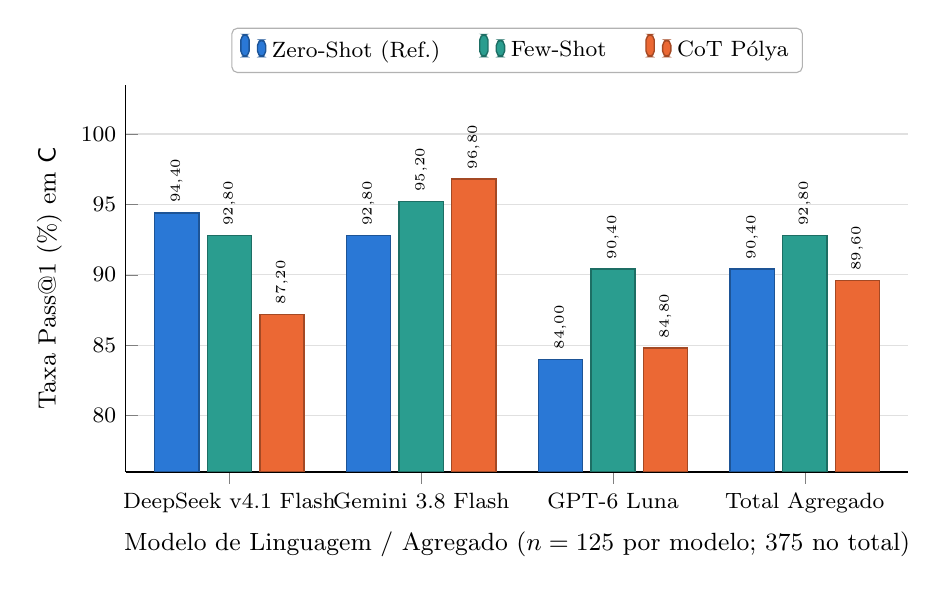
\begin{tikzpicture}
\begin{axis}[
  ybar=3pt,
  width=0.95\textwidth,
  height=6.5cm,
  bar width=16pt,
  ymin=76, ymax=103.5,
  ytick={80,85,90,95,100},
  ylabel={Taxa \passat{1} (\%) em \linguagem{C}},
  xlabel={Modelo de Linguagem / Agregado ($n=125$ por modelo; $375$ no total)},
  symbolic x coords={DeepSeek v4.1 Flash,Gemini 3.8 Flash,GPT-6 Luna,Total Agregado},
  xtick={DeepSeek v4.1 Flash,Gemini 3.8 Flash,GPT-6 Luna,Total Agregado},
  enlarge x limits=0.18,
  ymajorgrids=true,
  grid style={black!12},
  axis lines*=left,
  tick label style={font=\footnotesize},
  label style={font=\small},
  legend style={
    at={(0.5,1.03)},
    anchor=south,
    legend columns=3,
    draw=black!30,
    rounded corners=2pt,
    font=\footnotesize,
    /tikz/every even column/.append style={column sep=12pt}
  },
  nodes near coords,
  nodes near coords style={
    font=\tiny\bfseries,
    black,
    rotate=90,
    anchor=west,
    /pgf/number format/fixed,
    /pgf/number format/fixed zerofill,
    /pgf/number format/precision=2,
    /pgf/number format/use comma
  }
]
\addplot[fill=vAzul, draw=vAzul!70!black, line width=0.5pt] coordinates {
  (DeepSeek v4.1 Flash,94.40) (Gemini 3.8 Flash,92.80) (GPT-6 Luna,84.00) (Total Agregado,90.40)
};
\addplot[fill=vTeal, draw=vTeal!70!black, line width=0.5pt] coordinates {
  (DeepSeek v4.1 Flash,92.80) (Gemini 3.8 Flash,95.20) (GPT-6 Luna,90.40) (Total Agregado,92.80)
};
\addplot[fill=vLaranja, draw=vLaranja!70!black, line width=0.5pt] coordinates {
  (DeepSeek v4.1 Flash,87.20) (Gemini 3.8 Flash,96.80) (GPT-6 Luna,84.80) (Total Agregado,89.60)
};
\legend{Zero-Shot (Ref.), Few-Shot, CoT Pólya}
\end{axis}
\end{tikzpicture}

\caption[Pass@1 em C por estratégia de prompting na PP4]{Comparação da taxa \passat{1} em \linguagem{C} ($T=0$) entre \textit{Zero-Shot}, \textit{Few-Shot} e \textit{CoT Pólya}, individualmente e no agregado das $375$ execuções.}
\label{fig:res-pp4-pass1}
\end{figure}
\FloatBarrier

Ao verificar a taxa $\passat{1}$ na Figura~\ref{fig:res-pp4-pass1}, observa-se que no agregado da estratégia \textit{Few-Shot} (\promptname{few\_shot\_c.txt}, Apêndice~\ref{ap:prompts}) em relação ao \textit{baseline} houve uma melhora de $+2{,}40\text{ p.p.}$ ($90{,}40\% \rightarrow 92{,}80\%$), mostrando que a técnica que possui exemplos de códigos em \linguagem{C} apoia na construção de novas soluções. Em contrapartida, na técnica de cadeia de pensamento (\promptname{chain\_of\_thought\_polya.txt}, Apêndice~\ref{ap:prompts}), no agregado não houve melhora na taxa bruta ($89{,}60\%$), mesmo com o objetivo de fazer os modelos realizarem essa busca pelo conhecimento do problema. Apoiada pela metodologia de Pólya para resolver problemas matemáticos, essa abordagem foi adaptada para este estudo em computação em quatro etapas: Compreensão, Planejamento, Codificação (Execução) e Teste.

\begin{table}[!htbp]
\centering
\caption[Comparativo em C entre Zero-Shot, Few-Shot e CoT Pólya]{Comparativo em \linguagem{C} ($T = 0$) entre \textit{Zero-Shot}, \textit{Few-Shot} e \textit{CoT Pólya}.}
\label{tab:res-pp4-comparativo}
\resizebox{\textwidth}{!}{%
\begin{tabular}{@{}llcccccccc@{}}
\toprule
\textbf{Estratégia} & \textbf{Modelo} & \textbf{AC} & \textbf{Taxa \passat{1}} & \textbf{$\Delta$ AC} & \textbf{WA} & \textbf{RE} & \textbf{TLE} & \textbf{MLE} & \textbf{CE} \\
\midrule
\promptname{Zero-Shot} & DeepSeek v4.1 Flash & $118$ & $94{,}40\%$ & Ref. & $3$  & $1$ & $0$ & $0$ & $3$  \\
\promptname{Zero-Shot} & Gemini 3.8 Flash    & $116$ & $92{,}80\%$ & Ref. & $6$  & $0$ & $0$ & $0$ & $3$  \\
\promptname{Zero-Shot} & GPT-6 Luna          & $105$ & $84{,}00\%$ & Ref. & $15$ & $0$ & $0$ & $0$ & $5$  \\
\textbf{Zero-Shot}     & \textbf{Agregado (375)} & \textbf{339} & \textbf{90,40\%} & \textbf{Ref.} & \textbf{24} & \textbf{1} & \textbf{0} & \textbf{0} & \textbf{11} \\
\midrule
\promptname{Few-Shot}  & DeepSeek v4.1 Flash & $116$ & $92{,}80\%$ & $-2$ & $5$  & $0$ & $0$ & $0$ & $4$  \\
\promptname{Few-Shot}  & Gemini 3.8 Flash    & \tsecond{119} & \tsecond{95,20\%} & $+3$ & $6$  & $0$ & $0$ & $0$ & $0$  \\
\promptname{Few-Shot}  & GPT-6 Luna          & \tsecond{113} & \tsecond{90,40\%} & \textbf{$+8$} & $10$ & $1$ & $1$ & $0$ & $0$  \\
\textbf{Few-Shot}      & \textbf{Agregado (375)} & \tfirst{348} & \tfirst{92,80\%} & \tfirst{+9} & \textbf{21} & \textbf{1} & \textbf{1} & \textbf{0} & \tfirst{4} \\
\midrule
\promptname{CoT Pólya} & DeepSeek v4.1 Flash & $109$ & $87{,}20\%$ & $-9$ & $3$  & $0$ & $0$ & $0$ & $13$ \\
\promptname{CoT Pólya} & Gemini 3.8 Flash    & \tfirst{121} & \tfirst{96,80\%} & \tfirst{+5} & $4$  & $0$ & $0$ & $0$ & $0$  \\
\promptname{CoT Pólya} & GPT-6 Luna          & $106$ & $84{,}80\%$ & $+1$ & $10$ & $0$ & $0$ & $0$ & $9$  \\
\textbf{CoT Pólya}     & \textbf{Agregado (375)} & \textbf{336} & \textbf{89,60\%} & \textbf{$-3$} & \tfirst{17} & \textbf{0} & \textbf{0} & \textbf{0} & \textbf{22} \\
\bottomrule
\end{tabular}%
}
\end{table}

Ao observar as classificações não-\veredito{AC} na Tabela~\ref{tab:res-pp4-comparativo}, notou-se que, embora o \textit{CoT Pólya} tenha reduzido as falhas lógicas (\veredito{WA} caiu de 24 para 17 no agregado), ele teve um impacto direto no \textbf{DeepSeek v4.1 Flash}, além do \textbf{GPT-6 Luna}, principalmente em erros de compilação (\veredito{CE}). Ao verificar as respostas produzidas pelos dois modelos, constatou-se que elas estavam com mais de um bloco Markdown, o que contaminava a extração na hora de o sistema verificar o código. Mesmo deixando explícito na etapa de Codificação (Execução) que deveria haver um único bloco Markdown com a resposta em \linguagem{C}, os modelos produziam textos de explicação sobre o problema, ainda que isso guiasse melhor o raciocínio ao resolver as questões. Para mitigar isso, seria necessária uma mesclagem de \textit{prompts} mostrando no final exemplos do formato de saída esperado. Contudo, o \textbf{Gemini 3.8 Flash} conseguiu atingir \veredito{AC} em 121 questões (96,80\%), mostrando que alguns modelos conseguem seguir rigorosamente a instrução da etapa de codificação.

\begin{table}[!htbp]
\centering
\caption[Telemetria média de tokens, custo total e custo por AC na PP4]{Telemetria média de \textit{tokens}, custo total nas $125$ questões e custo por \veredito{AC} na PP4 (\linguagem{C}, $T = 0$).}
\label{tab:res-pp4-custos}
\resizebox{\textwidth}{!}{%
\begin{tabular}{@{}llrrrr@{}}
\toprule
\textbf{Estratégia} & \textbf{LLM} & \textbf{Tokens Ent. (média)} & \textbf{Tokens Saída (média)} & \textbf{Custo Total (USD)} & \textbf{Custo / AC (USD/AC)} \\
\midrule
\promptname{Zero-Shot} & DeepSeek v4.1 Flash & $923{,}9$   & $9.870{,}5$ & \$0,7406 & \$0,00628 \\
\promptname{Zero-Shot} & Gemini 3.8 Flash    & $873{,}2$   & $508{,}1$   & \$0,3200 & \$0,00276 \\
\promptname{Zero-Shot} & GPT-6 Luna          & $811{,}4$   & $1.681{,}0$ & \$0,1152 & \$0,00110 \\
\midrule
\promptname{Few-Shot}  & DeepSeek v4.1 Flash & $2.040{,}3$ & $9.964{,}2$ & \$0,7481 & \$0,00645 \\
\promptname{Few-Shot}  & Gemini 3.8 Flash    & $2.064{,}0$ & $537{,}9$   & \$0,4456 & \$0,00374 \\
\promptname{Few-Shot}  & GPT-6 Luna          & $1.877{,}2$ & $1.371{,}6$ & \$0,1092 & \$0,00097 \\
\midrule
\promptname{CoT Pólya} & DeepSeek v4.1 Flash & $1.460{,}6$ & $9.872{,}7$ & \$0,7410 & \$0,00680 \\
\promptname{CoT Pólya} & Gemini 3.8 Flash    & $1.380{,}0$ & $1.726{,}8$ & \$0,9388 & \$0,00776 \\
\promptname{CoT Pólya} & GPT-6 Luna          & $1.303{,}2$ & $2.450{,}7$ & \$0,1695 & \$0,00160 \\
\bottomrule
\end{tabular}%
}
\end{table}

Na Tabela~\ref{tab:res-pp4-custos}, é observável que a melhor técnica em custo-benefício foi a \textit{Few-Shot}, enquanto no \textit{CoT Pólya} houve um acréscimo tanto na quantidade de \textit{tokens} quanto, consequentemente, no custo por solução aceita (\veredito{AC}). Então, se existe uma busca em maximizar a corretude dos problemas, é recomendável utilizar o \textbf{Gemini 3.8 Flash}, lembrando que a temperatura é igual a zero ($T = 0{,}0$) para esses experimentos. Mais informações sobre o desempenho por fase da OBI, a auditoria dos erros de extração e os tempos de CPU desta etapa encontram-se no Apêndice~\ref{ap:resultados-complementares} (Seção~\ref{ap:pp4-detalhes}).

Por isso, nas linguagens que são mais desafiadoras para os modelos, torna-se mais interessante utilizar técnicas de \textit{prompt} para guiar a geração do código. No contexto da base de dados utilizada para este estudo, o \textbf{Gemini 3.8 Flash} atingiu o teto de 121 questões acertadas (96,80\%), a primeira vez na PP1 com a linguagem \linguagem{Python} e agora na PP4 com a linguagem \linguagem{C}.

\section{PP5: Evolução Geracional sob Paridade de Juiz}\label{sec:res-rq5}

Encerrando as análises experimentais, a partir do estudo preliminar~\citep{angelo2026ise} desenvolvido em conjunto com a equipe \textit{GEMA-LAB}, no qual a geração de código utilizou a mesma configuração deste TCC, porém com modelos de gerações anteriores (\textbf{Gemini 3.1 Pro} e \textbf{GPT-5.4}), identificaram-se as 46 questões do Nível Sênior da OBI (2016--2025) submetidas em \linguagem{Python} \textit{Zero-Shot} para consolidar a evolução dos modelos das famílias Google e OpenAI.

Para eliminar qualquer viés de avaliação, os códigos do estudo anterior foram rejulgados no mesmo \textit{Judge} utilizado neste trabalho, conforme detalhado na Seção~\ref{sec:met-rq5}, obtendo-se os vereditos comparativos sob as mesmas condições experimentais. Além disso, como a família DeepSeek não possui esse recorte em~\citet{angelo2026ise}, ela não participa desta comparação.

\begin{table}[!htbp]
\centering
\caption[Evolução intrafamília direta na PP5]{Comparação intrafamília direta entre geração anterior e geração atual ($n = 46$, \linguagem{Python} \textit{Zero-Shot}).}
\label{tab:res-pp5-intrafamilia}
\small
\resizebox{\textwidth}{!}{%
\begin{tabular}{@{}llcccc@{}}
\toprule
\textbf{Família} & \textbf{Evolução (Anterior $\rightarrow$ Atual)} & \textbf{AC (de 46)} & \textbf{$\Delta$ \passat{1}} & \textbf{$\Delta$ Tokens} & \textbf{Custo / AC (US\$)} \\
\midrule
Gemini & Gemini 3.1 Pro $\rightarrow$ Gemini 3.8 Flash & $45 \rightarrow 44$ ($-1$) & $-2{,}18\text{ p.p.}$  & $-51{,}2\%$ & $\$0{,}06356 \rightarrow \$0{,}00226$ \\
GPT    & GPT-5.4 $\rightarrow$ GPT-6 Luna              & $31 \rightarrow 38$ ($+7$) & $+15{,}22\text{ p.p.}$ & $+69{,}5\%$ & $\$0{,}00972 \rightarrow \$0{,}00083$ \\
\bottomrule
\end{tabular}%
}
\end{table}

Nota-se que a Tabela~\ref{tab:res-pp5-intrafamilia} traz um recorte interessante sobre os quatro modelos: enquanto nos modelos da OpenAI houve um desempenho melhor ($31 \rightarrow 38$ acertos, $+15{,}22\text{ p.p.}$), nos modelos do Google o resultado manteve-se estável ($45 \rightarrow 44$ acertos). Além disso, as duas gerações de modelos foram lançadas no ano de 2026, mostrando que em pouco tempo os modelos estão melhorando sua capacidade na geração de código.

\begin{figure}[!htbp]
\centering
% Gráfico de barras agrupadas: Pass@1 (%) por etapa oficial da OBI Sênior na PP5 (Cap. 5, Seção 5.6.2)
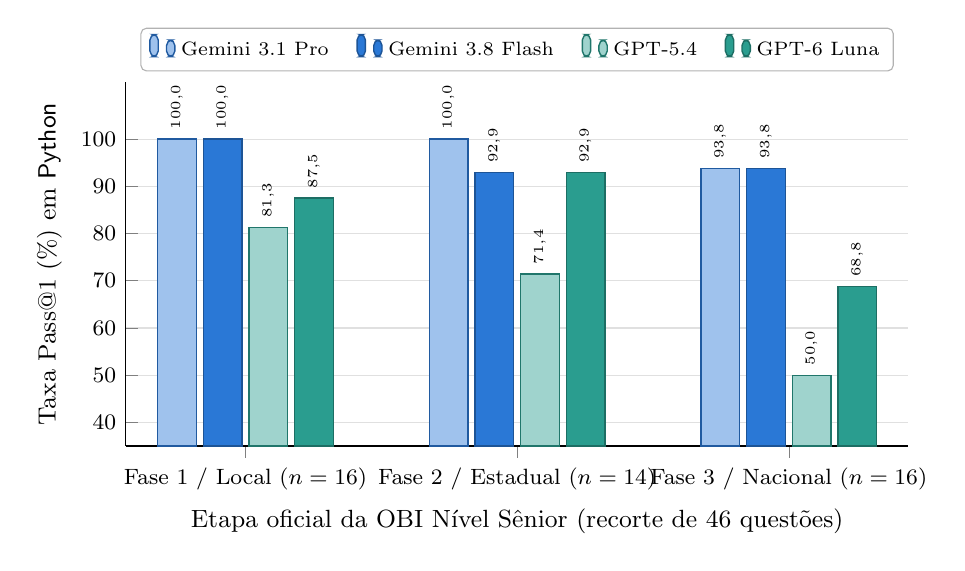
\begin{tikzpicture}
\begin{axis}[
  ybar=2.5pt,
  width=0.95\textwidth,
  height=6.2cm,
  bar width=14pt,
  ymin=35, ymax=112,
  ytick={40,50,60,70,80,90,100},
  ylabel={Taxa \passat{1} (\%) em \linguagem{Python}},
  xlabel={Etapa oficial da OBI Nível Sênior (recorte de 46 questões)},
  symbolic x coords={Fase1,Fase2,Fase3},
  xtick={Fase1,Fase2,Fase3},
  xticklabels={Fase 1 / Local ($n=16$),Fase 2 / Estadual ($n=14$),Fase 3 / Nacional ($n=16$)},
  enlarge x limits=0.22,
  ymajorgrids=true,
  grid style={black!12},
  axis lines*=left,
  tick label style={font=\footnotesize},
  label style={font=\small},
  legend style={
    at={(0.5,1.03)},
    anchor=south,
    legend columns=4,
    draw=black!30,
    rounded corners=2pt,
    font=\scriptsize,
    /tikz/every even column/.append style={column sep=8pt}
  },
  nodes near coords,
  nodes near coords style={
    font=\tiny\bfseries,
    black,
    rotate=90,
    anchor=west,
    /pgf/number format/fixed,
    /pgf/number format/fixed zerofill,
    /pgf/number format/precision=1,
    /pgf/number format/use comma
  }
]
\addplot[fill=vAzul!45, draw=vAzul!75!black, line width=0.5pt] coordinates {
  (Fase1,100.0) (Fase2,100.0) (Fase3,93.75)
};
\addplot[fill=vAzul, draw=vAzul!70!black, line width=0.5pt] coordinates {
  (Fase1,100.0) (Fase2,92.86) (Fase3,93.75)
};
\addplot[fill=vTeal!45, draw=vTeal!75!black, line width=0.5pt] coordinates {
  (Fase1,81.25) (Fase2,71.43) (Fase3,50.0)
};
\addplot[fill=vTeal, draw=vTeal!70!black, line width=0.5pt] coordinates {
  (Fase1,87.5) (Fase2,92.86) (Fase3,68.75)
};
\legend{Gemini 3.1 Pro, Gemini 3.8 Flash, GPT-5.4, GPT-6 Luna}
\end{axis}
\end{tikzpicture}

\caption[Desempenho por etapa oficial da OBI Sênior na PP5]{Taxa \passat{1} (\%) em \linguagem{Python} \textit{Zero-Shot} estratificada pelas três etapas oficiais da OBI Nível Sênior ($n = 46$).}
\label{fig:res-pp5-fases}
\end{figure}
\FloatBarrier

Ao verificar o desempenho em relação às fases da OBI, como mostra a Figura~\ref{fig:res-pp5-fases}, existe uma melhora significativa para os modelos da OpenAI. Sendo que as questões da Fase Estadual (Fase~2) e da Fase Nacional (Fase~3) são consideradas as que têm maior dificuldade, foi justamente nelas que houve um aumento expressivo no $\passat{1}$.

\begin{figure}[!htbp]
\centering
% Gráficos lado a lado: Fronteira de Pareto (Custo/AC vs. Pass@1) e Tokens médios por questão na PP5 (Cap. 5, Seção 5.6.3)
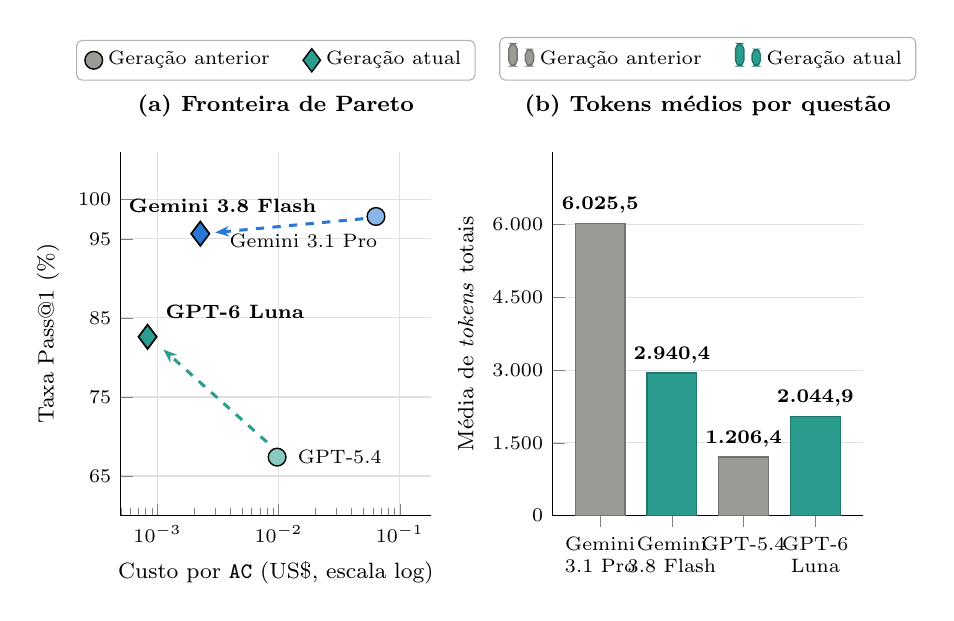
\begin{tikzpicture}
\begin{groupplot}[
  group style={
    group size=2 by 1,
    horizontal sep=1.55cm
  },
  width=0.455\textwidth,
  height=6.2cm,
  ymajorgrids=true,
  grid style={black!12},
  axis lines*=left,
  tick label style={font=\scriptsize},
  label style={font=\footnotesize},
  title style={font=\footnotesize\bfseries, yshift=3pt}
]
% Painel (a): Deslocamento da Fronteira de Pareto (Custo/AC em escala log vs. Pass@1)
\nextgroupplot[
  xmode=log,
  xmajorgrids=true,
  title={(a) Fronteira de Pareto},
  xlabel={Custo por \veredito{AC} (US\$, escala log)},
  ylabel={Taxa \passat{1} (\%)},
  xmin=0.0005, xmax=0.18,
  ymin=60, ymax=106,
  ytick={65,75,85,95,100},
  legend to name=legpp5pareto,
  legend style={
    legend columns=2,
    draw=black!30,
    rounded corners=2pt,
    font=\scriptsize,
    /tikz/every even column/.append style={column sep=10pt}
  }
]
% Entradas de legenda neutras (forma distingue geração)
\addlegendimage{only marks, mark=*, mark size=3.2pt, mark options={fill=vCinza, draw=black, line width=0.5pt}}
\addlegendentry{Geração anterior}
\addlegendimage{only marks, mark=diamond*, mark size=4.2pt, mark options={fill=vTeal, draw=black, line width=0.5pt}}
\addlegendentry{Geração atual}

% Pontos reais coloridos por família (Gemini = vAzul, GPT = vTeal)
\addplot[only marks, mark=*, mark size=3.2pt, mark options={fill=vAzul!55, draw=black, line width=0.5pt}, forget plot]
  coordinates {(0.06356,97.83)};
\addplot[only marks, mark=diamond*, mark size=4.4pt, mark options={fill=vAzul, draw=black, line width=0.6pt}, forget plot]
  coordinates {(0.00226,95.65)};
\addplot[only marks, mark=*, mark size=3.2pt, mark options={fill=vTeal!55, draw=black, line width=0.5pt}, forget plot]
  coordinates {(0.00972,67.39)};
\addplot[only marks, mark=diamond*, mark size=4.4pt, mark options={fill=vTeal, draw=black, line width=0.6pt}, forget plot]
  coordinates {(0.00083,82.61)};

% Setas tracejadas indicando a evolução intrafamília
\draw[-{Stealth[length=5pt]}, dashed, line width=1.1pt, color=vAzul]
  (axis cs:0.050,97.55) -- (axis cs:0.0030,95.80);
\draw[-{Stealth[length=5pt]}, dashed, line width=1.1pt, color=vTeal]
  (axis cs:0.0080,69.3) -- (axis cs:0.00112,81.0);

% Rótulos dos modelos sem sobreposição
\node[font=\scriptsize, anchor=north east, yshift=-3pt, xshift=4pt] at (axis cs:0.06356,97.83) {Gemini 3.1 Pro};
\node[font=\scriptsize\bfseries, anchor=south, yshift=4pt, xshift=8pt] at (axis cs:0.00226,95.65) {Gemini 3.8 Flash};
\node[font=\scriptsize, anchor=west, xshift=4pt] at (axis cs:0.00972,67.39) {GPT-5.4};
\node[font=\scriptsize\bfseries, anchor=south west, xshift=3pt, yshift=3pt] at (axis cs:0.00083,82.61) {GPT-6 Luna};

% Painel (b): Consumo médio de tokens totais por questão
\nextgroupplot[
  ybar,
  bar shift=0pt,
  bar width=18pt,
  title={(b) Tokens médios por questão},
  symbolic x coords={G31,G38,GPT54,GPT6},
  xtick={G31,G38,GPT54,GPT6},
  xticklabels={Gemini\\3.1 Pro,Gemini\\3.8 Flash,GPT-5.4,GPT-6\\Luna},
  x tick label style={align=center},
  enlarge x limits=0.22,
  ymin=0, ymax=7500,
  scaled y ticks=false,
  ytick={0,1500,3000,4500,6000},
  ylabel={Média de \textit{tokens} totais},
  yticklabel style={/pgf/number format/fixed, /pgf/number format/1000 sep={.}},
  legend to name=legpp5tokens,
  legend style={
    legend columns=2,
    draw=black!30,
    rounded corners=2pt,
    font=\scriptsize,
    /tikz/every even column/.append style={column sep=10pt}
  }
]
\addplot[fill=vCinza, draw=vCinza!75!black, line width=0.5pt] coordinates {
  (G31,6025.5) (GPT54,1206.4)
};
\addplot[fill=vTeal, draw=vTeal!75!black, line width=0.5pt] coordinates {
  (G38,2940.4) (GPT6,2044.9)
};
\legend{Geração anterior, Geração atual}

% Rótulos numéricos centralizados acima de cada barra
\node[font=\scriptsize\bfseries, anchor=south] at (axis cs:G31,6025.5) {6.025,5};
\node[font=\scriptsize\bfseries, anchor=south] at (axis cs:G38,2940.4) {2.940,4};
\node[font=\scriptsize\bfseries, anchor=south] at (axis cs:GPT54,1206.4) {1.206,4};
\node[font=\scriptsize\bfseries, anchor=south] at (axis cs:GPT6,2044.9) {2.044,9};
\end{groupplot}

% Legendas acima de cada painel
\node[anchor=south] at ($(group c1r1.north) + (0,0.78cm)$)
  {\pgfplotslegendfromname{legpp5pareto}};
\node[anchor=south] at ($(group c2r1.north) + (0,0.78cm)$)
  {\pgfplotslegendfromname{legpp5tokens}};
\end{tikzpicture}

\caption[Fronteira de Pareto e consumo médio de tokens na PP5]{Eficiência econômica e verbosidade nas $46$ questões em \linguagem{Python} \textit{Zero-Shot}: (a) deslocamento intrafamília na fronteira de Pareto (custo por \veredito{AC} em escala logarítmica versus \passat{1}) e (b) consumo médio de \textit{tokens} totais por problema.}
\label{fig:res-pp5-pareto-tokens}
\end{figure}
\FloatBarrier

Como se pode perceber na Tabela~\ref{tab:res-pp5-intrafamilia}, o modelo \textbf{Gemini 3.8 Flash} é cerca de 28 vezes mais barato por solução aceita que o modelo \textbf{Gemini 3.1 Pro}; além disso, o modelo \textbf{GPT-6 Luna} é cerca de 11 vezes mais barato que o modelo \textbf{GPT-5.4}. A Figura~\ref{fig:res-pp5-pareto-tokens} evidencia que os modelos atuais possuem eficiência econômica, mesmo produzindo mais \textit{tokens}, como no caso do \textbf{GPT-6 Luna}, mostrando que os modelos atuais estão tendo um custo-benefício melhor na geração de código. O detalhamento completo dos vereditos, da paridade de julgamento e das 16 questões com divergência na PP5 encontra-se no Apêndice~\ref{ap:resultados-complementares} (Seção~\ref{ap:pp5-detalhes}).

\section{Ameaças à Validade e Principais Contribuições}\label{sec:res-sintese}

Os resultados do \textit{benchmark} realizado nos cenários em relação aos cinco modelos analisados possuem um prazo de validade, pois em algum momento esses modelos poderão ser descontinuados. Outro ponto importante é que, para reproduzir os resultados deste estudo, a máquina deve possuir a mesma configuração descrita na Seção~\ref{sec:met-judge} para garantir a fidelidade da avaliação.

Por outro lado, as principais contribuições estão na proposta de uma arquitetura para avaliação de LLMs por meio de requisições de API, na qual podem ser utilizados vários tipos de \textit{datasets} de programação competitiva para avaliar os modelos. No contexto de construir sistemas que façam requisições aos LLMs, a ferramenta \texttt{competitive-programming-bench}~\citep{compbench2026} possui um grande valor para um sistema tutor inteligente voltado à programação competitiva, mostrando questões que podem representar uma barreira na geração de código para os LLMs, como a questão \textit{Construção de Rodovia} do \textit{dataset} deste estudo. Assim, a ferramenta consegue realizar uma execução local para avaliação da geração de código, armazenando \textit{prompts}, quantidades de \textit{tokens}, código produzido, entre outros fatores.

\cleardoublepage

\chapter{Conclusão}\label{cap:conclusao}

Retomando o objetivo geral de avaliar experimentalmente a capacidade dos LLMs na resolução de problemas do Nível Sênior da OBI (Modalidade Programação), este estudo trouxe cinco cenários nos quais, dentro da configuração utilizada de temperatura zero ($T = 0{,}0$) e apenas uma requisição ($\passat{1}$), os modelos divergem quanto à abordagem de melhor desempenho. No cenário da PP1, o \textbf{DeepSeek v4.1 Flash} e o \textbf{Gemini 3.8 Flash} mostraram uma amplitude menor de variação para questões e \textit{prompts} puramente textuais. Em sequência, para elementos visuais (PP2), no \textbf{DeepSeek v4.1 Flash} houve degradação comparativamente aos outros dois modelos na linguagem de melhor desempenho geral (\linguagem{C++}); isso mostra que modelos multimodais nem sempre conseguem performar bem com imagens no formato Base64 (\modalidade{img}), observando-se que o desempenho melhora quando existem descrições textuais das imagens (\modalidade{description}). Na avaliação de restrições (PP3), verificou-se que na linguagem mais sensível (\linguagem{C}) os modelos acabaram tratando como ruído informações que são importantes para os competidores da OBI (Modalidade Programação, Nível Sênior), como o limite de memória e o limite de tempo. Nesse caso de linguagens que precisam de maior cuidado na geração de código (PP4), notou-se que a aplicação de técnicas de \textit{prompt} é uma boa alternativa, destacando-se o \textit{Few-Shot} como melhor custo-benefício. Além disso, na comparação geracional (PP5), mostrou-se que os modelos de uma mesma família estão melhorando o custo-benefício e a geração de código para cenários de programação competitiva.

Por consequência, este Trabalho de Conclusão de Curso trouxe contribuições como uma base estruturada e validada por oráculo de 125 problemas do Nível Sênior da OBI (2016--2025) com 4.681 casos de teste, uma proposta de arquitetura experimental, uma ferramenta executável localmente e um \textit{benchmark} na resolução de problemas algorítmicos, alinhado às referências da literatura~\citep{chen2021evaluating,li2022competition,zheng2025livecodebench,alcantara2025assessing}. Para o cenário educacional, utilizar LLMs como motor de raciocínio em sistemas tutores inteligentes exige verificar se os modelos conseguem auxiliar os alunos, e não substituí-los, como mostram os estudos de~\citet{priyanka2025development,peng2025enhancing}.

Assim, como trabalhos futuros, a ferramenta pode ser expandida para avaliações em outros tipos de \textit{datasets} de problemas de programação competitiva, com perspectivas de utilização na geração de código em relação à métrica $\passat{k}$ e variando a temperatura, buscando avaliar a ``criatividade'' dos modelos. Além disso, vislumbra-se incorporar mecanismos de autocorreção para códigos já produzidos anteriormente, podendo evoluir para um sistema multiagente que utilize a metodologia de Pólya --- com cada agente dedicado a uma etapa do ciclo de resolução de problemas (Compreensão, Planejamento, Codificação (Execução) e Teste) ---, comunicando-se entre si por meio de protocolos bem definidos.

\cleardoublepage

% % % % % % % % % % % % % % % % % % % % % % % % % % %
% Referências Bibliográficas                         %
% % % % % % % % % % % % % % % % % % % % % % % % % % %
\label{sec:referencias}

% Atualiza o cabeçalho no \chapter* da bibliografia no estilo myheadings
\markboth{\bibname}{\bibname}

\bibliography{Ref/Referencias}


% % % % % % % % % % % % % % % % % % % % % % % % % % %
% Apêndices                                            %
% % % % % % % % % % % % % % % % % % % % % % % % % % %
\cleardoublepage
\appendix
\chapter{\texorpdfstring{\textit{Prompts}}{Prompts} Utilizados nos Experimentos}\label{ap:prompts}

Este apêndice reproduz integralmente os três modelos de \textit{prompt} empregados nas rodadas experimentais descritas no Capítulo~\ref{cap:metodologia}. As variáveis entre chaves (\texttt{\{language\}}, \texttt{\{problem\}}, \texttt{\{time\_limit\}} e \texttt{\{memory\_limit\}}) são preenchidas dinamicamente pelo módulo \texttt{PromptBuilder} no momento de cada submissão.

\section*{A.1 \textit{Prompt Zero-Shot} (\texttt{zero\_shot.txt})}

\begin{small}
\VerbatimInput[breaklines, breakanywhere, fontsize=\footnotesize, frame=single, framesep=2mm, rulecolor=\color{black!40}]{Apendices/prompts/zero_shot.txt}
\end{small}

\section*{A.2 \textit{Prompt Few-Shot} em C (\texttt{few\_shot\_c.txt})}

\begin{small}
\VerbatimInput[breaklines, breakanywhere, fontsize=\footnotesize, frame=single, framesep=2mm, rulecolor=\color{black!40}]{Apendices/prompts/few_shot_c.txt}
\end{small}

\section*{A.3 \textit{Prompt Chain-of-Thought} -- Metodologia de Pólya (\texttt{chain\_of\_thought\_polya.txt})}

\begin{small}
\VerbatimInput[breaklines, breakanywhere, fontsize=\footnotesize, frame=single, framesep=2mm, rulecolor=\color{black!40}]{Apendices/prompts/chain_of_thought_polya.txt}
\end{small}

\chapter{Esquema de Dados e Registros de Execução}\label{ap:esquema-dados}

Este apêndice documenta a organização de diretórios e os esquemas de dados adotados na base experimental \texttt{database/dataset\_obi\_senior/}, bem como o formato dos registros acumulativos em JSON e das planilhas consolidadas em CSV gerados durante a execução dos experimentos em \texttt{results/dataset\_obi\_senior/}.

\section{Estrutura da Base de Questões e Esquema \texttt{problem.json}}\label{ap:esquema-problem}

Na base \texttt{database/dataset\_obi\_senior/}, cada um dos 125 problemas do Nível Sênior da OBI (2016--2025) é armazenado em um diretório próprio nomeado com o título oficial da questão (ou acrescido do ano em caso de homonímia entre edições, como \texttt{Chuva\_2019} e \texttt{Chuva\_2022}). A estrutura interna de cada diretório organiza-se em quatro elementos padronizados:

\begin{itemize}
    \item \texttt{problem.json}: arquivo principal com o enunciado estruturado, especificações de entrada e saída, restrições, exemplos, figuras associadas e metadados da prova;
    \item \texttt{imgs/}: subdiretório contendo os arquivos de imagem (\texttt{.png} ou \texttt{.jpg}) extraídos do caderno oficial, presente nas 46 questões multimodais;
    \item \texttt{solutions/}: subdiretório com as soluções humanas de referência disponibilizadas pela organização da OBI (\texttt{.cpp}, \texttt{.c}, \texttt{.py}, \texttt{.java} ou \texttt{.js}), utilizadas na validação em modo oráculo;
    \item \texttt{test\_cases/inputs/} e \texttt{test\_cases/outputs/}: subdiretórios contendo os pares de arquivos de entrada (\texttt{.in}) e saída esperada (\texttt{.out}) dos 4.681 casos de teste oficiais.
\end{itemize}

A Tabela~\ref{tab:ap-esquema-problem} descreve os campos que compõem o arquivo \texttt{problem.json} validado pelo modelo de dados \texttt{Problem} (\texttt{src/models/problem.py}).

\begin{table}[!htbp]
\centering
\caption[Campos do esquema problem.json da base OBI Sênior]{Descrição dos campos que compõem o esquema \texttt{problem.json} de cada questão da base.}
\label{tab:ap-esquema-problem}
\small
\resizebox{\textwidth}{!}{%
\begin{tabular}{@{}llp{9.2cm}@{}}
\toprule
\textbf{Campo} & \textbf{Tipo} & \textbf{Descrição} \\
\midrule
\texttt{title}             & \texttt{string}         & Título oficial do problema no caderno de prova da OBI. \\
\texttt{statement}         & \texttt{string}         & Texto principal do enunciado, contendo marcadores \texttt{[nome\_img]} na posição original das figuras. \\
\texttt{input}             & \texttt{string}         & Especificação do formato dos dados fornecidos na entrada padrão (\texttt{stdin}). \\
\texttt{output}            & \texttt{string}         & Especificação do formato exigido na saída padrão (\texttt{stdout}). \\
\texttt{constraints}       & \texttt{string}         & Restrições matemáticas e intervalos numéricos das variáveis de entrada. \\
\texttt{examples}          & \texttt{list[object]}   & Lista de pares \texttt{\{"input": ..., "output": ...\}} com os exemplos públicos do enunciado. \\
\texttt{imgs}              & \texttt{list[string]}   & Lista com os nomes dos arquivos de imagem localizados no subdiretório \texttt{imgs/}. \\
\texttt{imgs\_description} & \texttt{object / list}  & Mapeamento de cada imagem para sua descrição textual estruturada, empregado na modalidade \modalidade{description}. \\
\texttt{rating}            & \texttt{list[int]}      & Pontuação das submissões ou subtarefas previstas no caderno oficial (ex.: \texttt{[100]}). \\
\texttt{year}              & \texttt{string}         & Ano da edição da OBI à qual a questão pertence (2016 a 2025). \\
\texttt{level}             & \texttt{string}         & Nível da modalidade Programação (\texttt{"senior"}). \\
\texttt{period}            & \texttt{string}         & Etapa seletiva da competição (\textit{Fase 1 / Local}, \textit{Fase 2 / Estadual} ou \textit{Fase 3 / Nacional}). \\
\texttt{topics}            & \texttt{list[string]}   & Tópicos algorítmicos associados à questão segundo a ementa da OBI. \\
\texttt{time\_limit}       & \texttt{float}          & Tempo máximo de execução permitido por caso de teste, em segundos. \\
\texttt{memory\_limit}     & \texttt{int}            & Consumo máximo de memória RAM permitido durante a execução, em megabytes (MB). \\
\bottomrule
\end{tabular}%
}
\end{table}

A seguir, apresenta-se um exemplo real de arquivo \texttt{problem.json} referente à questão \textit{Acelerador de partículas} (OBI 2020, Fase Local):

\begin{small}
\begin{Verbatim}[breaklines, breakanywhere, fontsize=\footnotesize, frame=single, framesep=2mm, rulecolor=\color{black!40}]
{
    "title": "Acelerador de partículas",
    "statement": "A universidade está inaugurando um grande acelerador de partículas, com um emissor e três sensores, numerados 1, 2 e 3. [...] A figura mostra o caminho por onde as partículas trafegam, com uma graduação de 1 quilômetro. Por exemplo, do emissor até o acelerador são 3 quilômetros e a circunferência do acelerador tem 8 quilômetros.\n[1.png]\nNeste problema, será dada a distância total, em quilômetros, percorrida por uma certa partícula trafegando do emissor até algum sensor e seu programa deve determinar qual sensor foi atingido pela partícula.",
    "input": "A entrada consiste de apenas uma linha contendo um inteiro D, representando a distância total percorrida pela partícula.",
    "output": "Seu programa deve imprimir uma linha contendo um inteiro, representando o número do sensor que a partícula atingiu.",
    "constraints": "6 ≤ D ≤ 800008\nD sempre será a distância total percorrida entre o emissor e algum sensor.",
    "examples": [
        { "input": "23", "output": "2" },
        { "input": "6", "output": "1" },
        { "input": "9192", "output": "3" }
    ],
    "imgs": ["1.png"],
    "rating": [100],
    "year": "2020",
    "level": "senior",
    "period": "Fase Local",
    "topics": ["matemática", "aritmética modular", "simulação"],
    "time_limit": 5.0,
    "memory_limit": 256,
    "imgs_description": {
        "1.png": "[Descrição da imagem: Diagrama esquemático do acelerador de partículas. À esquerda, há um emissor retangular do qual parte um tubo reto horizontal em direção ao leste com comprimento de 3 km, marcado com traços a cada 1 km. No ponto de 3 km, o tubo conecta-se tangencialmente à parte inferior de um acelerador circular de 8 km de circunferência [...]]"
    }
}
\end{Verbatim}
\end{small}

\section{Estrutura dos Registros Acumulativos de Execução (\texttt{.json})}\label{ap:esquema-execucao}

Durante as baterias experimentais, o módulo \texttt{Orchestrator} armazena o histórico completo de cada submissão em arquivos JSON organizados hierarquicamente pelo caminho \texttt{results/dataset\_obi\_senior/<modelo>/<prompt>/<linguagem>/<modalidade>/<questao>.json}. Cada arquivo contém uma lista de objetos JSON em que cada elemento registra uma tentativa de resolução e seu respectivo julgamento local, conforme especificado na Tabela~\ref{tab:ap-esquema-execucao}.

\begin{table}[!htbp]
\centering
\caption[Campos do registro JSON acumulativo de execução]{Estrutura de campos dos arquivos JSON gerados por questão em cada bateria experimental.}
\label{tab:ap-esquema-execucao}
\small
\resizebox{\textwidth}{!}{%
\begin{tabular}{@{}llp{9.2cm}@{}}
\toprule
\textbf{Campo} & \textbf{Tipo} & \textbf{Descrição} \\
\midrule
\texttt{attempt}          & \texttt{int}    & Índice sequencial da tentativa registrada para a questão naquela configuração. \\
\texttt{timestamp}        & \texttt{string} & Data e horário UTC da conclusão da requisição no padrão ISO~8601. \\
\texttt{model}            & \texttt{string} & Identificador do modelo consultado na API (ex.: \texttt{gemini-3.8-flash}). \\
\texttt{prompt\_name}     & \texttt{string} & Nome do modelo de \textit{prompt} aplicado (\texttt{zero\_shot}, \texttt{few\_shot\_c} ou \texttt{chain\_of\_thought\_polya}). \\
\texttt{prompt}           & \texttt{string} & Texto integral do \textit{prompt} formatado enviado ao modelo na requisição. \\
\texttt{language}         & \texttt{string} & Linguagem-alvo da submissão (\texttt{python}, \texttt{c}, \texttt{cpp}, \texttt{java} ou \texttt{javascript}). \\
\texttt{modality}         & \texttt{string} & Modalidade de representação visual adotada (\texttt{text}, \texttt{img} ou \texttt{description}). \\
\texttt{include\_limits}  & \texttt{bool}   & Indica se os limites de tempo e memória foram injetados explicitamente no \textit{prompt}. \\
\texttt{time\_limit}      & \texttt{float}  & Limite de tempo de execução configurado no \texttt{JudgeService} (em segundos). \\
\texttt{memory\_limit}    & \texttt{int}    & Limite de memória configurado no \texttt{JudgeService} (em MB). \\
\texttt{tokens}           & \texttt{object} & Contagem de \textit{tokens} da chamada: \texttt{input\_tokens}, \texttt{output\_tokens} e \texttt{total\_tokens}. \\
\texttt{cost\_usd}        & \texttt{object} & Custo financeiro em dólares (USD): \texttt{input\_cost}, \texttt{output\_cost} e \texttt{total\_cost}. \\
\texttt{raw\_response}    & \texttt{string} & Resposta textual bruta retornada pela API do modelo. \\
\texttt{extracted\_code}  & \texttt{string} & Código-fonte limpo extraído do bloco Markdown para compilação e teste. \\
\texttt{judge\_result}    & \texttt{object} & Resultado da avaliação local contendo o veredito final (\texttt{judge\_predict}), o maior tempo de execução entre os testes (\texttt{execution\_time}), a contagem por veredito (\texttt{counts}) e o total de casos avaliados (\texttt{total\_test\_cases}). \\
\bottomrule
\end{tabular}%
}
\end{table}

O trecho a seguir exemplifica um registro JSON produzido para a questão \textit{Acelerador de partículas} em linguagem \linguagem{C}:

\begin{small}
\begin{Verbatim}[breaklines, breakanywhere, fontsize=\footnotesize, frame=single, framesep=2mm, rulecolor=\color{black!40}]
[
    {
        "attempt": 1,
        "timestamp": "2026-11-18T02:26:26.250617+00:00",
        "model": "deepseek/deepseek-v4.1-flash",
        "prompt_name": "chain_of_thought_polya",
        "prompt": "Você é um programador competitivo experiente em C. [...]",
        "language": "c",
        "modality": "text",
        "include_limits": false,
        "time_limit": 5.0,
        "memory_limit": 256,
        "tokens": {
            "input_tokens": 1143,
            "output_tokens": 3226,
            "total_tokens": 4369
        },
        "cost_usd": {
            "input_cost": 3e-06,
            "output_cost": 0.001936,
            "total_cost": 0.001939
        },
        "raw_response": "## 1. COMPREENSÃO DO PROBLEMA [...] ```c\n#include <stdio.h>\nint main(void) { ... }\n``` [...]",
        "extracted_code": "#include <stdio.h>\n\nint main(void) {\n    long long D;\n    if (scanf(\"%lld\", &D) != 1) return 0;\n    int r = (int)(D % 8);\n    if (r == 6) printf(\"1\\n\");\n    else if (r == 7) printf(\"2\\n\");\n    else printf(\"3\\n\");\n    return 0;\n}",
        "judge_result": {
            "judge_predict": "AC",
            "execution_time": 0.1003995,
            "counts": { "AC": 39, "WA": 0, "RE": 0, "TLE": 0, "MLE": 0, "CE": 0 },
            "total_test_cases": 39
        }
    }
]
\end{Verbatim}
\end{small}

\section{Formato das Tabelas CSV Consolidadas}\label{ap:esquema-csv}

Além dos registros detalhados em JSON, o ambiente persiste tabelas em formato CSV para sumarização direta dos vereditos e da telemetria em \texttt{results/dataset\_obi\_senior/}. Existem dois padrões de arquivos tabulares:

\begin{enumerate}
    \item \textbf{Tabelas de julgamento (\texttt{oracle.csv} e \texttt{judge/*.csv}):} consolidam o resultado do \texttt{JudgeService} por questão em cada bateria experimental. Cada linha corresponde a uma submissão avaliada e contém dez colunas:
    \begin{itemize}
        \item \texttt{question\_name}: identificador da questão na base;
        \item \texttt{execution\_time}: tempo máximo de execução (em segundos) registrado entre os casos de teste da questão;
        \item \texttt{judge\_predict}: veredito final atribuído à submissão (\veredito{AC}, \veredito{WA}, \veredito{RE}, \veredito{TLE}, \veredito{MLE} ou \veredito{CE});
        \item \texttt{AC}, \texttt{WA}, \texttt{RE}, \texttt{TLE}, \texttt{MLE}, \texttt{CE}: quantidade de casos de teste individuais classificados em cada categoria de veredito;
        \item \texttt{total\_test\_cases}: número total de casos de teste oficiais aferidos na questão.
    \end{itemize}
    \item \textbf{Tabela de comparação entre gerações (\texttt{llms\_compare.csv}):} reúne, para as 46 questões com figuras avaliadas na PP5 em \linguagem{Python} \textit{Zero-Shot}, a coluna \texttt{question\_name} seguida pelas triplas de colunas \texttt{veredito\_<modelo>}, \texttt{tokens\_<modelo>} (soma de \textit{tokens} da requisição) e \texttt{custo\_<modelo>} (custo em USD) para os modelos das gerações anterior e atual sob paridade de juiz.
\end{enumerate}

\chapter{Resultados Complementares}\label{ap:resultados-complementares}

Este apêndice reúne as tabelas e figuras que aprofundam as análises do Capítulo~\ref{cap:resultados}, concentrando-se nos desdobramentos que não foram detalhados no corpo principal do texto: cobertura complementar entre linguagens, distribuição de vereditos por modelo, telemetria de tamanho de código e custo, mapeamento nominal das questões com transição de veredito e auditoria dos erros de extração.

\section{Detalhamento Complementar da PP1: Desempenho por Linguagem}\label{ap:pp1-detalhes}

\subsection{Taxa de Acerto (\texorpdfstring{\passat{1}}{Pass@1}) e Cobertura Complementar}\label{sec:res-rq1-pass1}

A Tabela~\ref{tab:res-pp1-pass1} apresenta os números absolutos e percentuais de aprovação (\veredito{AC} de 125) de cada modelo nas cinco linguagens avaliadas, servindo de referência numérica para a Figura~\ref{fig:res-pp1-ac-linguagem} discutida na Seção~\ref{sec:res-rq1}.

\begin{table}[!htbp]
\centering
\caption[Taxa de acerto Pass@1 por modelo e linguagem na PP1]{Quantidade absoluta de aprovações (\veredito{AC} de 125) e taxa $\passat{1}$ (\%) por modelo e linguagem de programação ($T = 0{,}0$).}
\label{tab:res-pp1-pass1}
\small
\resizebox{\textwidth}{!}{%
\begin{tabular}{lccccccc}
\toprule
Modelo & Python & C & C++ & Java & JavaScript & Média ($\passat{1}$) & Total AC (625) \\
\midrule
DeepSeek v4.1 Flash & \tsecond{118} (94,40\%) & \tfirst{118} (94,40\%) & \tfirst{121} (96,80\%) & \tsecond{117} (93,60\%) & \tsecond{115} (92,00\%) & \tsecond{117,8} (94,24\%) & \tsecond{589} \\
Gemini 3.8 Flash    & \tfirst{121} (96,80\%)  & \tsecond{117} (93,60\%) & \tsecond{119} (95,20\%) & 114 (91,20\%) & \tfirst{119} (95,20\%)  & \tfirst{118,0} (94,40\%)  & \tfirst{590}  \\
GPT-6 Luna          & 109 (87,20\%)           & 110 (88,00\%)           & 113 (90,40\%)           & \tfirst{119} (95,20\%)  & \tsecond{115} (92,00\%) & 113,2 (90,56\%)           & 566           \\
\midrule
\rowcolor{linhaDestaque}\textbf{Agregado (de 375)} & 348 (92,80\%) & 345 (92,00\%) & \tfirst{353} (94,13\%) & \tsecond{350} (93,33\%) & 349 (93,07\%) & -- & 1.745 (93,07\%) \\
\bottomrule
\end{tabular}%
}
\par\smallskip{\footnotesize \tfirst{Vermelho} e \tsecond{azul}: melhor e segundo melhor valor por coluna.}
\end{table}

Além das medidas de dispersão apresentadas na Tabela~\ref{tab:res-pp1-estabilidade} do Capítulo~\ref{cap:resultados}, um aspecto relevante é verificar se os modelos erram sempre as mesmas questões ou se as falhas mudam conforme a linguagem escolhida. A Tabela~\ref{tab:ap-pp1-estabilidade} mostra a cobertura complementar de cada LLM sobre o conjunto de 125 problemas. Embora o número de questões resolvidas de forma unânime nas cinco linguagens (5/5) varie entre 92 (no \textbf{GPT-6 Luna}) e 105 (no \textbf{DeepSeek v4.1 Flash} e no \textbf{Gemini 3.8 Flash}), todos os modelos conseguem resolver entre 123 e 124 questões ($98{,}4\%$ a $99{,}2\%$) quando se considera o acerto em ao menos uma linguagem ($\ge 1$). Esse comportamento reforça que a grande maioria dos erros pontuais na PP1 não decorre da falta de capacidade lógica para resolver o problema, mas de tropeços específicos na sintaxe ou nas particularidades de implementação de cada linguagem.

\begin{table}[!htbp]
\centering
\caption[Cobertura complementar entre linguagens na PP1]{Cobertura complementar de resolução de cada modelo ao longo das cinco linguagens sobre as 125 questões da OBI Sênior.}
\label{tab:ap-pp1-estabilidade}
\small
\resizebox{\textwidth}{!}{%
\begin{tabular}{lccc}
\toprule
Modelo & Acertos nas 5 Linguagens (5/5) & Acerto em ao menos 1 ($\ge 1$) & Erro nas 5 Linguagens (0/5) \\
\midrule
DeepSeek v4.1 Flash & \tfirst{105/125} (84,00\%) & 123/125 (98,40\%)          & 2/125 (1,60\%) \\
Gemini 3.8 Flash    & \tfirst{105/125} (84,00\%) & \tfirst{124/125} (99,20\%) & \tfirst{1/125} (0,80\%) \\
GPT-6 Luna          & 92/125 (73,60\%)           & \tfirst{124/125} (99,20\%) & \tfirst{1/125} (0,80\%) \\
\bottomrule
\end{tabular}%
}
\end{table}

\subsection{Distribuição de Vereditos por Modelo e Linguagem}\label{sec:res-rq1-falhas}

Enquanto o Capítulo~\ref{cap:resultados} (Tabela~\ref{tab:res-pp1-erros-lang}) sintetizou os erros por linguagem de programação, a Tabela~\ref{tab:res-pp1-vereditos-llm} e a Figura~\ref{fig:res-pp1-erros-linguagem} mostram como esses vereditos se dividem entre os três LLMs nas 625 submissões de cada modelo.

\begin{table}[!htbp]
\centering
\caption[Distribuição geral dos vereditos por LLM na PP1]{Distribuição geral dos vereditos do \textit{JudgeService} por LLM nas 625 execuções da PP1 ($T = 0{,}0$).}
\label{tab:res-pp1-vereditos-llm}
\small
\resizebox{\textwidth}{!}{%
\begin{tabular}{lccccccc}
\toprule
Modelo & \chip{corAC}\veredito{AC} & \chip{corWA}\veredito{WA} & \chip{corRE}\veredito{RE} & \chip{corTLE}\veredito{TLE} & \chip{corMLE}\veredito{MLE} & \chip{corCE}\veredito{CE} & Total \\
\midrule
DeepSeek v4.1 Flash & 589 (94,2\%) & 23 (3,7\%) & 1 (0,2\%) & 1 (0,2\%) & 0 (0,0\%) & 11 (1,8\%) & 625 \\
Gemini 3.8 Flash    & 590 (94,4\%) & 24 (3,8\%) & 4 (0,6\%) & 0 (0,0\%) & 2 (0,3\%) & 5 (0,8\%)  & 625 \\
GPT-6 Luna          & 566 (90,6\%) & 47 (7,5\%) & 2 (0,3\%) & 3 (0,5\%) & 1 (0,2\%) & 6 (1,0\%)  & 625 \\
\bottomrule
\end{tabular}%
}
\end{table}

\begin{figure}[!htbp]
\centering
% Gráfico de barras empilhadas: distribuição de erros (Não-AC) por linguagem (Cap. 5, Seção 5.2.2)
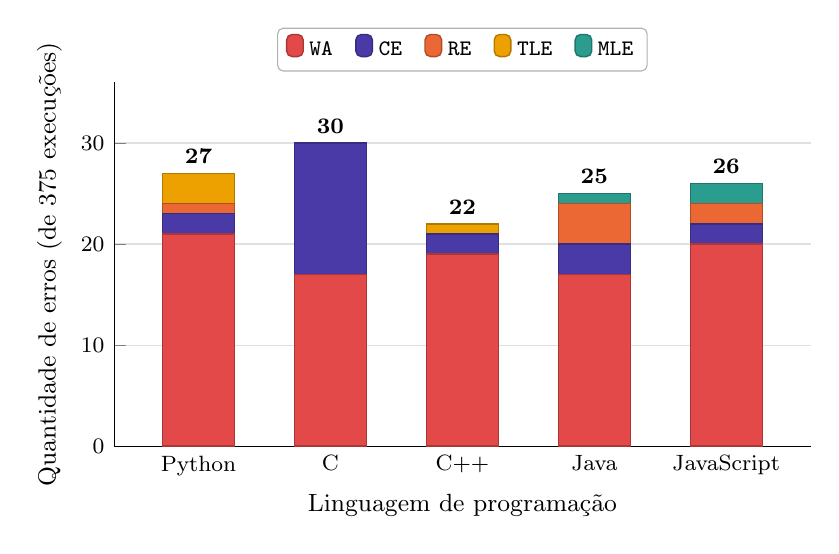
\begin{tikzpicture}
\begin{axis}[
  ybar stacked,
  width=0.86\textwidth,
  height=6.2cm,
  bar width=26pt,
  ymin=0, ymax=36,
  ylabel={Quantidade de erros (de 375 execuções)},
  xlabel={Linguagem de programação},
  symbolic x coords={Python,C,C++,Java,JavaScript},
  xtick=data,
  enlarge x limits=0.16,
  ymajorgrids=true,
  grid style={black!12},
  axis lines*=left,
  tick label style={font=\footnotesize},
  label style={font=\small},
  legend style={
    at={(0.5,1.03)},
    anchor=south,
    legend columns=5,
    draw=black!30,
    rounded corners=2pt,
    font=\footnotesize,
    /tikz/every even column/.append style={column sep=6pt}
  }
]
\addplot[fill=corWA, draw=corWA!75!black, line width=0.5pt] coordinates {
  (Python,21) (C,17) (C++,19) (Java,17) (JavaScript,20)
};
\addplot[fill=corCE, draw=corCE!75!black, line width=0.5pt] coordinates {
  (Python,2) (C,13) (C++,2) (Java,3) (JavaScript,2)
};
\addplot[fill=corRE, draw=corRE!75!black, line width=0.5pt] coordinates {
  (Python,1) (C,0) (C++,0) (Java,4) (JavaScript,2)
};
\addplot[fill=corTLE, draw=corTLE!75!black, line width=0.5pt] coordinates {
  (Python,3) (C,0) (C++,1) (Java,0) (JavaScript,0)
};
\addplot[fill=corMLE, draw=corMLE!75!black, line width=0.5pt] coordinates {
  (Python,0) (C,0) (C++,0) (Java,1) (JavaScript,2)
};
\legend{\veredito{WA}, \veredito{CE}, \veredito{RE}, \veredito{TLE}, \veredito{MLE}}

% Totais agregados acima de cada barra empilhada
\node[font=\footnotesize\bfseries, anchor=south] at (axis cs:Python,27) {27};
\node[font=\footnotesize\bfseries, anchor=south] at (axis cs:C,30) {30};
\node[font=\footnotesize\bfseries, anchor=south] at (axis cs:C++,22) {22};
\node[font=\footnotesize\bfseries, anchor=south] at (axis cs:Java,25) {25};
\node[font=\footnotesize\bfseries, anchor=south] at (axis cs:JavaScript,26) {26};
\end{axis}
\end{tikzpicture}

\caption[Distribuição agregada de erros por linguagem na PP1]{Distribuição agregada dos erros (não-\veredito{AC}) por linguagem de programação nas 375 execuções de cada linguagem.}
\label{fig:res-pp1-erros-linguagem}
\end{figure}
\FloatBarrier

Cruzando os vereditos por modelo e linguagem, notam-se comportamentos bem característicos. A linguagem \linguagem{C} concentrou 13 dos 22 erros de compilação (\veredito{CE}) de toda a bateria --- incluindo todos os 5 \veredito{CE}s registrados pelo \textbf{Gemini 3.8 Flash} ---, devido à exigência de inclusão explícita de cabeçalhos e manipulação manual de memória. Já no \textbf{DeepSeek v4.1 Flash}, a inspeção dos arquivos de saída revelou que os seus 11 \veredito{CE}s (\linguagem{Python}: 2; \linguagem{C}: 4; \linguagem{C++}: 1; \linguagem{Java}: 2; \linguagem{JavaScript}: 2) ocorreram porque o modelo atingiu o teto de $131.072$ \textit{tokens} ainda durante o raciocínio interno, encerrando a resposta antes de emitir o bloco de código. Por fim, \linguagem{Python} concentrou 3 dos 4 casos de \veredito{TLE} por conta do custo de interpretação em laços extensos, ao passo que \linguagem{Java} reuniu 4 dos 7 erros em tempo de execução (\veredito{RE}), geralmente ligados à leitura de entrada ou estouro de limites de vetores e pilha.

\subsection{Extensão do Código, Consumo de \textit{Tokens}, Custo e Tempo de CPU}\label{sec:res-rq1-eficiencia}

A Tabela~\ref{tab:res-pp1-eficiencia} detalha as médias de linhas de código (LOC), número de caracteres, \textit{tokens} de saída, custo acumulado em dólares e tempo médio de CPU das soluções aprovadas para cada par modelo--linguagem (dados que originaram a Figura~\ref{fig:res-pp1-loc-tempo} do Capítulo~\ref{cap:resultados}).

\begin{table}[!htbp]
\centering
\caption[Métricas de código, tokens, custo e tempo de CPU na PP1]{Extensão média do código (LOC e caracteres), \textit{tokens} médios de saída, custo total (USD) e tempo médio de CPU nas soluções \veredito{AC} por modelo e linguagem.}
\label{tab:res-pp1-eficiencia}
\small
\resizebox{\textwidth}{!}{%
\begin{tabular}{llrrrrr}
\toprule
Modelo & Linguagem & LOC Médio & Caracteres Médio & \textit{Tokens} Saída Médio & Custo Total (USD) & Tempo Médio \veredito{AC} (s) \\
\midrule
DeepSeek v4.1 Flash & Python     & 42,6 & 911,2   & 8.688,1  & \$0,6519 & 0,2776 \\
DeepSeek v4.1 Flash & C          & 58,7 & 1.259,8 & 11.387,3 & \$0,8544 & 0,1569 \\
DeepSeek v4.1 Flash & C++        & 49,9 & 1.073,1 & 7.541,5  & \$0,5659 & 0,1856 \\
DeepSeek v4.1 Flash & Java       & 60,8 & 1.684,8 & 8.939,3  & \$0,6708 & 0,1365 \\
DeepSeek v4.1 Flash & JavaScript & 46,8 & 1.027,4 & 9.198,4  & \$0,6902 & 0,0929 \\
\midrule
Gemini 3.8 Flash    & Python     & 47,6 & 1.151,9 & 435,6    & \$0,2828 & 0,2973 \\
Gemini 3.8 Flash    & C          & 60,9 & 1.334,5 & 531,8    & \$0,3280 & 0,1360 \\
Gemini 3.8 Flash    & C++        & 53,9 & 1.172,7 & 486,1    & \$0,3065 & 0,1811 \\
Gemini 3.8 Flash    & Java       & 77,7 & 2.209,4 & 668,0    & \$0,3918 & 0,1213 \\
Gemini 3.8 Flash    & JavaScript & 67,9 & 1.658,8 & 565,2    & \$0,3436 & 0,0742 \\
\midrule
GPT-6 Luna          & Python     & 34,2 & 778,5   & 1.361,0  & \$0,0948 & 0,3595 \\
GPT-6 Luna          & C          & 56,4 & 1.316,7 & 1.527,8  & \$0,1053 & 0,1734 \\
GPT-6 Luna          & C++        & 47,3 & 1.071,9 & 1.242,5  & \$0,0874 & 0,2048 \\
GPT-6 Luna          & Java       & 72,3 & 2.066,4 & 1.597,5  & \$0,1096 & 0,1517 \\
GPT-6 Luna          & JavaScript & 46,4 & 1.040,8 & 1.414,2  & \$0,0982 & 0,1326 \\
\bottomrule
\end{tabular}%
}
\end{table}

Os números da Tabela~\ref{tab:res-pp1-eficiencia} mostram como o esforço de geração difere entre os modelos. No \textbf{DeepSeek v4.1 Flash}, a necessidade de construir estruturas de dados manualmente em \linguagem{C} fez a média de saída subir para $11.387{,}3$ \textit{tokens} por questão (contra $7.541{,}5$ em \linguagem{C++}, onde a STL já oferece essas estruturas prontas), resultando em um gasto de US\$\,0,8544 apenas nessa linguagem e US\$\,3,4333 no somatório das cinco baterias. Já o \textbf{Gemini 3.8 Flash} emitiu respostas diretas com média global de $537{,}4$ \textit{tokens} de saída (custo total de US\$\,1,6527), enquanto o \textbf{GPT-6 Luna} apresentou a operação mais econômica da PP1, somando US\$\,0,4953 para avaliar todas as 625 submissões.
\FloatBarrier

\section{Detalhamento Complementar da PP2: Impacto Visual e Modalidades}\label{ap:pp2-detalhes}

\subsection{Contraste entre Questões com e sem Imagens no \textit{Baseline}}\label{sec:res-rq2-baseline}

Para verificar em que medida a presença de figuras no enunciado original afeta os modelos quando submetidos apenas ao texto puro (\modalidade{text}, $T = 0$), a Tabela~\ref{tab:res-pp2-baseline} e a Figura~\ref{fig:res-pp2-img-noimg} comparam o desempenho entre as 46 questões que possuem imagens e as 79 questões puramente textuais. O comparativo é apresentado sob dois recortes: na melhor linguagem individual de cada LLM na PP1 (\linguagem{C++} para o DeepSeek, \linguagem{Python} para o Gemini e \linguagem{Java} para o GPT-6 Luna) e no somatório das cinco linguagens.

\begin{table}[!htbp]
\centering
\caption{Desempenho no \textit{baseline} (\modalidade{text}, $T=0$) entre questões com e sem imagens.}
\label{tab:res-pp2-baseline}
\resizebox{\textwidth}{!}{%
\begin{tabular}{@{}llccccl@{}}
\toprule
\textbf{Recorte} & \textbf{LLM} & \textbf{Ling.} & \textbf{Com Imagens} & \textbf{Sem Imagens} & \textbf{Dif. (p.p.)} & \textbf{Erros (Com Img.)} \\
\midrule
Melhor linguagem  & DeepSeek v4.1 Flash & C++    & $44/46$ ($95{,}65\%$)  & $77/79$ ($97{,}47\%$)  & $-1{,}82$ & $1$ \veredito{WA}, $1$ \veredito{CE} \\
Melhor linguagem  & Gemini 3.8 Flash    & Python & $44/46$ ($95{,}65\%$)  & $77/79$ ($97{,}47\%$)  & $-1{,}82$ & $2$ \veredito{WA} \\
Melhor linguagem  & GPT-6 Luna          & Java   & $42/46$ ($91{,}30\%$)  & $77/79$ ($97{,}47\%$)  & $-6{,}16$ & $4$ \veredito{WA} \\
\midrule
Agregado (5 ling.) & DeepSeek v4.1 Flash & Todas  & $212/230$ ($92{,}17\%$) & $377/395$ ($95{,}44\%$) & $-3{,}27$ & --- \\
Agregado (5 ling.) & Gemini 3.8 Flash    & Todas  & $213/230$ ($92{,}61\%$) & $377/395$ ($95{,}44\%$) & $-2{,}83$ & --- \\
Agregado (5 ling.) & GPT-6 Luna          & Todas  & $201/230$ ($87{,}39\%$) & $365/395$ ($92{,}41\%$) & $-5{,}01$ & --- \\
\bottomrule
\end{tabular}%
}
\end{table}

\begin{figure}[!htbp]
\centering
% Gráfico comparativo: Com Imagens (46) vs Sem Imagens (79) no baseline textual (Cap. 5, Seção 5.3.1)
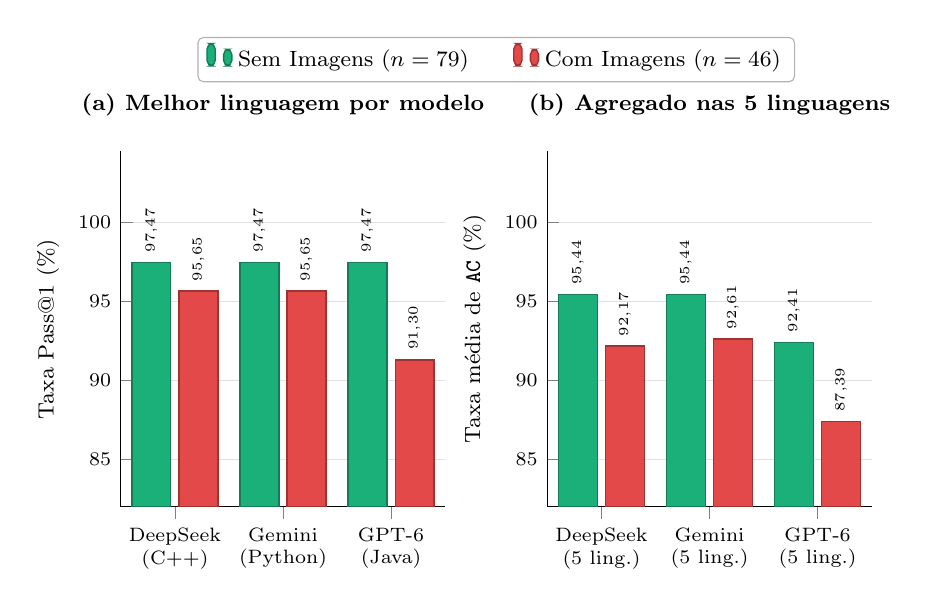
\begin{tikzpicture}
\begin{groupplot}[
  group style={
    group size=2 by 1,
    horizontal sep=1.3cm
  },
  width=0.47\textwidth,
  height=6.1cm,
  symbolic x coords={DeepSeek,Gemini,GPT6},
  xtick={DeepSeek,Gemini,GPT6},
  enlarge x limits=0.25,
  ymajorgrids=true,
  grid style={black!12},
  axis lines*=left,
  tick label style={font=\scriptsize},
  x tick label style={align=center},
  label style={font=\footnotesize},
  title style={font=\footnotesize\bfseries, yshift=3pt},
  ymin=82, ymax=104.5,
  ytick={85,90,95,100}
]
% Painel (a): Melhor linguagem individual
\nextgroupplot[
  ybar=3pt,
  bar width=14pt,
  title={(a) Melhor linguagem por modelo},
  ylabel={Taxa \passat{1} (\%)},
  xticklabels={DeepSeek\\(C++),Gemini\\(Python),GPT-6\\(Java)},
  legend to name=legpp2imgnoimg,
  legend style={
    legend columns=2,
    draw=black!30,
    rounded corners=2pt,
    font=\footnotesize,
    /tikz/every even column/.append style={column sep=14pt}
  },
  nodes near coords,
  nodes near coords style={
    font=\tiny\bfseries,
    black,
    rotate=90,
    anchor=west,
    /pgf/number format/fixed,
    /pgf/number format/fixed zerofill,
    /pgf/number format/precision=2,
    /pgf/number format/use comma
  }
]
\addplot[fill=vVerde, draw=vVerde!70!black, line width=0.5pt] coordinates {
  (DeepSeek,97.47) (Gemini,97.47) (GPT6,97.47)
};
\addplot[fill=vVermelho, draw=vVermelho!70!black, line width=0.5pt] coordinates {
  (DeepSeek,95.65) (Gemini,95.65) (GPT6,91.30)
};
\legend{Sem Imagens ($n=79$), Com Imagens ($n=46$)}

% Painel (b): Agregado nas 5 linguagens
\nextgroupplot[
  ybar=3pt,
  bar width=14pt,
  title={(b) Agregado nas 5 linguagens},
  ylabel={Taxa média de \veredito{AC} (\%)},
  xticklabels={DeepSeek\\(5 ling.),Gemini\\(5 ling.),GPT-6\\(5 ling.)},
  nodes near coords,
  nodes near coords style={
    font=\tiny\bfseries,
    black,
    rotate=90,
    anchor=west,
    /pgf/number format/fixed,
    /pgf/number format/fixed zerofill,
    /pgf/number format/precision=2,
    /pgf/number format/use comma
  }
]
\addplot[fill=vVerde, draw=vVerde!70!black, line width=0.5pt] coordinates {
  (DeepSeek,95.44) (Gemini,95.44) (GPT6,92.41)
};
\addplot[fill=vVermelho, draw=vVermelho!70!black, line width=0.5pt] coordinates {
  (DeepSeek,92.17) (Gemini,92.61) (GPT6,87.39)
};
\end{groupplot}

% Legenda compartilhada acima dos dois gráficos
\node[anchor=south] at ($(group c1r1.north)!0.5!(group c2r1.north) + (0,0.75cm)$)
  {\pgfplotslegendfromname{legpp2imgnoimg}};
\end{tikzpicture}

\caption[Contraste entre questões com e sem imagens na PP2]{Taxa de aprovação (\passat{1}) no \textit{baseline} textual (\modalidade{text}) para questões com e sem imagens (a) na melhor linguagem de cada LLM e (b) no agregado das cinco linguagens.}
\label{fig:res-pp2-img-noimg}
\end{figure}
\FloatBarrier

Nas 79 questões puramente textuais, os três modelos convergiram para exatamente $77/79$ acertos ($97{,}47\%$) em suas melhores linguagens. Quando avaliados nos 46 problemas cujos cadernos originais trazem figuras --- frequentemente usadas para ilustrar malhas, tabuleiros, cortes geométricos ou ligações em grafos ---, a taxa de aprovação recua em todos os cenários ($-1{,}82\text{ p.p.}$ a $-6{,}16\text{ p.p.}$ na melhor linguagem, e $-2{,}83\text{ p.p.}$ a $-5{,}01\text{ p.p.}$ no agregado das cinco linguagens), confirmando que a ausência da referência visual dificulta a interpretação espacial do enunciado.

\subsection{Transições de Veredito e Telemetria de Custos nas Modalidades Visuais}\label{sec:res-rq2-custo}

No experimento controlado em \linguagem{C++} sobre as 46 questões com imagens (Seção~\ref{sec:res-rq2}), o tempo médio de execução das soluções no \textit{JudgeService} manteve-se praticamente inalterado entre as modalidades \modalidade{text}, \modalidade{img} e \modalidade{description} (variando apenas entre $0{,}164\,\mathrm{s}$ e $0{,}187\,\mathrm{s}$). Das 46 questões avaliadas, 31 ($67{,}39\%$) receberam veredito \veredito{AC} unânime nos três modelos e nas três modalidades. As 15 questões que apresentaram variação de veredito ou falha em ao menos uma configuração estão listadas na Tabela~\ref{tab:res-pp2-divergencias}.

\begin{table}[!htbp]
\centering
\caption{Mapa de transições de vereditos nas $15$ questões com divergência ou falha em \linguagem{C++} (\modalidade{text} / \modalidade{img} / \modalidade{description}).}
\label{tab:res-pp2-divergencias}
\resizebox{\textwidth}{!}{%
\begin{tabular}{@{}lccc@{}}
\toprule
\textbf{Problema} & \textbf{DeepSeek v4.1 Flash} & \textbf{Gemini 3.8 Flash} & \textbf{GPT-6 Luna} \\
\midrule
Arco e flecha          & \veredito{AC} / \veredito{CE} / \veredito{AC} & \veredito{AC} / \veredito{AC} / \veredito{AC} & \veredito{AC} / \veredito{AC} / \veredito{AC} \\
Brigadeiros            & \veredito{AC} / \veredito{AC} / \veredito{WA} & \veredito{AC} / \veredito{AC} / \veredito{WA} & \veredito{WA} / \veredito{WA} / \veredito{WA} \\
Burocracia             & \veredito{AC} / \veredito{AC} / \veredito{AC} & \veredito{AC} / \veredito{AC} / \veredito{AC} & \veredito{AC} / \veredito{WA} / \veredito{WA} \\
Chuva\_2019            & \veredito{CE} / \veredito{AC} / \veredito{AC} & \veredito{AC} / \veredito{AC} / \veredito{AC} & \veredito{WA} / \veredito{AC} / \veredito{AC} \\
Construção de Rodovia  & \veredito{WA} / \veredito{WA} / \veredito{WA} & \veredito{WA} / \veredito{WA} / \veredito{WA} & \veredito{WA} / \veredito{WA} / \veredito{WA} \\
Cortando o Papel       & \veredito{AC} / \veredito{AC} / \veredito{AC} & \veredito{AC} / \veredito{AC} / \veredito{AC} & \veredito{WA} / \veredito{AC} / \veredito{AC} \\
Dario e Xerxes         & \veredito{AC} / \veredito{AC} / \veredito{AC} & \veredito{AC} / \veredito{AC} / \veredito{AC} & \veredito{WA} / \veredito{AC} / \veredito{AC} \\
Fast-Food              & \veredito{AC} / \veredito{AC} / \veredito{AC} & \veredito{WA} / \veredito{AC} / \veredito{AC} & \veredito{AC} / \veredito{AC} / \veredito{AC} \\
Frete                  & \veredito{AC} / \veredito{CE} / \veredito{AC} & \veredito{AC} / \veredito{AC} / \veredito{AC} & \veredito{AC} / \veredito{AC} / \veredito{AC} \\
Metrô da Nlogônia      & \veredito{AC} / \veredito{WA} / \veredito{AC} & \veredito{AC} / \veredito{AC} / \veredito{AC} & \veredito{AC} / \veredito{WA} / \veredito{WA} \\
Nova avenida           & \veredito{AC} / \veredito{AC} / \veredito{WA} & \veredito{AC} / \veredito{AC} / \veredito{AC} & \veredito{AC} / \veredito{AC} / \veredito{AC} \\
Passatempo             & \veredito{AC} / \veredito{AC} / \veredito{AC} & \veredito{AC} / \veredito{AC} / \veredito{AC} & \veredito{CE} / \veredito{WA} / \veredito{AC} \\
Soma                   & \veredito{AC} / \veredito{AC} / \veredito{AC} & \veredito{WA} / \veredito{WA} / \veredito{AC} & \veredito{AC} / \veredito{AC} / \veredito{AC} \\
Transportes            & \veredito{AC} / \veredito{CE} / \veredito{AC} & \veredito{AC} / \veredito{AC} / \veredito{AC} & \veredito{AC} / \veredito{AC} / \veredito{AC} \\
Trio de Bonecas        & \veredito{AC} / \veredito{AC} / \veredito{WA} & \veredito{AC} / \veredito{AC} / \veredito{AC} & \veredito{WA} / \veredito{WA} / \veredito{WA} \\
\bottomrule
\end{tabular}%
}
\end{table}

O mapa individualizado permite enxergar onde o recurso visual realmente ajudou. Questões com forte apelo espacial, como \textit{Chuva\_2019}, \textit{Cortando o Papel}, \textit{Dario e Xerxes} e \textit{Fast-Food}, passaram de erro para aprovação (\veredito{AC}) assim que os modelos receberam a imagem ou sua descrição. Em \textit{Passatempo} (no GPT-6 Luna) e \textit{Soma} (no Gemini 3.8 Flash), apenas a descrição estruturada (\modalidade{description}) foi capaz de conduzir ao acerto. Em contrapartida, no \textbf{DeepSeek v4.1 Flash}, questões que já eram resolvidas apenas com o texto (\textit{Arco e flecha}, \textit{Frete} e \textit{Transportes}) sofreram erro de compilação (\veredito{CE}) quando a imagem foi anexada em Base64, voltando a passar normalmente na modalidade descritiva.

A Tabela~\ref{tab:res-pp2-custos} complementa a Figura~\ref{fig:res-pp2-tokens-custo} do Capítulo~\ref{cap:resultados} com os valores numéricos exatos de \textit{tokens} médios de entrada e saída e o custo total das 46 questões em \linguagem{C++}. Nota-se que substituir a imagem em Base64 pela descrição textual evita o salto de \textit{tokens} de entrada no Gemini ($2.173{,}1 \rightarrow 1.046{,}6$) e o aumento da cadeia de saída no DeepSeek ($12.993{,}4 \rightarrow 5.639{,}5$), reduzindo o custo financeiro sem perda de acurácia.

\begin{table}[!htbp]
\centering
\caption{Consumo médio de \textit{tokens} por questão e custo total em dólares nas $46$ questões em \linguagem{C++} (PP2).}
\label{tab:res-pp2-custos}
\small
\resizebox{\textwidth}{!}{%
\begin{tabular}{@{}llrrr@{}}
\toprule
\textbf{LLM} & \textbf{Modalidade} & \textbf{Tokens Ent. (média)} & \textbf{Tokens Saída (média)} & \textbf{Custo Total (46 q.)} \\
\midrule
DeepSeek v4.1 Flash & \modalidade{text}        & $950{,}8$   & $8.598{,}9$  & \$0,2375 \\
DeepSeek v4.1 Flash & \modalidade{img}         & $1.181{,}3$ & $12.993{,}4$ & \$0,3588 \\
DeepSeek v4.1 Flash & \modalidade{description} & $1.110{,}0$ & $5.639{,}5$  & \$0,1558 \\
\midrule
Gemini 3.8 Flash    & \modalidade{text}        & $901{,}5$   & $454{,}5$    & \$0,1095 \\
Gemini 3.8 Flash    & \modalidade{img}         & $2.173{,}1$ & $482{,}4$    & \$0,1582 \\
Gemini 3.8 Flash    & \modalidade{description} & $1.046{,}6$ & $466{,}5$    & \$0,1166 \\
\midrule
GPT-6 Luna          & \modalidade{text}        & $838{,}2$   & $1.257{,}4$  & \$0,0328 \\
GPT-6 Luna          & \modalidade{img}         & $983{,}0$   & $1.370{,}8$  & \$0,0360 \\
GPT-6 Luna          & \modalidade{description} & $982{,}6$   & $1.125{,}9$  & \$0,0304 \\
\bottomrule
\end{tabular}%
}
\end{table}
\FloatBarrier

\section{Detalhamento Complementar da PP3: Limites de Tempo e Memória em C}\label{ap:pp3-detalhes}

\subsection{Transições de Veredito Questão a Questão}\label{sec:res-rq3-overeng}

A Figura~\ref{fig:res-pp3-erros} ilustra visualmente a migração de falhas entre o \textit{baseline} em \linguagem{C} e a bateria com limites explícitos (PP3). Como programas em \linguagem{C} compilados com \texttt{-O2} já rodam muito abaixo dos tetos da OBI (sem nenhum \veredito{TLE} ou \veredito{MLE}), informar \texttt{time\_limit} e \texttt{memory\_limit} no \textit{prompt} levou os modelos a tentarem otimizações desnecessárias de alocação e leitura, aumentando o total de respostas incorretas (\veredito{WA}).

\begin{figure}[!htbp]
\centering
% Gráfico em 3 painéis empilhados: distribuição de erros (Não-AC) Baseline vs PP3 em C (Cap. 5, Seção 5.4.1)
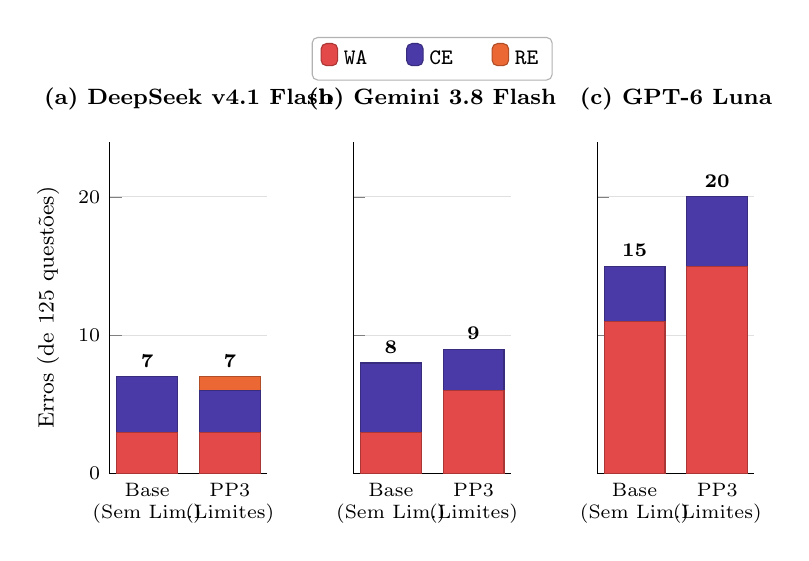
\begin{tikzpicture}
\begin{groupplot}[
  group style={
    group size=3 by 1,
    horizontal sep=1.1cm,
    yticklabels at=edge left
  },
  width=0.295\textwidth,
  height=5.8cm,
  symbolic x coords={Baseline,PP3},
  xtick={Baseline,PP3},
  xticklabels={Base\\(Sem Lim.),PP3\\(Limites)},
  x tick label style={align=center},
  enlarge x limits=0.45,
  ymajorgrids=true,
  grid style={black!12},
  axis lines*=left,
  tick label style={font=\scriptsize},
  label style={font=\footnotesize},
  title style={font=\footnotesize\bfseries, yshift=2pt},
  ymin=0, ymax=24
]
% Painel (a): DeepSeek v4.1 Flash
\nextgroupplot[
  ybar stacked,
  bar width=22pt,
  title={(a) DeepSeek v4.1 Flash},
  ylabel={Erros (de 125 questões)},
  legend to name=legpp3erros,
  legend style={
    legend columns=3,
    draw=black!30,
    rounded corners=2pt,
    font=\footnotesize,
    /tikz/every even column/.append style={column sep=12pt}
  }
]
\addplot[fill=corWA, draw=corWA!75!black, line width=0.4pt] coordinates {(Baseline,3) (PP3,3)};
\addplot[fill=corCE, draw=corCE!75!black, line width=0.4pt] coordinates {(Baseline,4) (PP3,3)};
\addplot[fill=corRE, draw=corRE!75!black, line width=0.4pt] coordinates {(Baseline,0) (PP3,1)};
\legend{\veredito{WA}, \veredito{CE}, \veredito{RE}}
\node[font=\scriptsize\bfseries, anchor=south] at (axis cs:Baseline,7) {7};
\node[font=\scriptsize\bfseries, anchor=south] at (axis cs:PP3,7) {7};

% Painel (b): Gemini 3.8 Flash
\nextgroupplot[
  ybar stacked,
  bar width=22pt,
  title={(b) Gemini 3.8 Flash}
]
\addplot[fill=corWA, draw=corWA!75!black, line width=0.4pt] coordinates {(Baseline,3) (PP3,6)};
\addplot[fill=corCE, draw=corCE!75!black, line width=0.4pt] coordinates {(Baseline,5) (PP3,3)};
\addplot[fill=corRE, draw=corRE!75!black, line width=0.4pt] coordinates {(Baseline,0) (PP3,0)};
\node[font=\scriptsize\bfseries, anchor=south] at (axis cs:Baseline,8) {8};
\node[font=\scriptsize\bfseries, anchor=south] at (axis cs:PP3,9) {9};

% Painel (c): GPT-6 Luna
\nextgroupplot[
  ybar stacked,
  bar width=22pt,
  title={(c) GPT-6 Luna}
]
\addplot[fill=corWA, draw=corWA!75!black, line width=0.4pt] coordinates {(Baseline,11) (PP3,15)};
\addplot[fill=corCE, draw=corCE!75!black, line width=0.4pt] coordinates {(Baseline,4) (PP3,5)};
\addplot[fill=corRE, draw=corRE!75!black, line width=0.4pt] coordinates {(Baseline,0) (PP3,0)};
\node[font=\scriptsize\bfseries, anchor=south] at (axis cs:Baseline,15) {15};
\node[font=\scriptsize\bfseries, anchor=south] at (axis cs:PP3,20) {20};
\end{groupplot}

% Legenda compartilhada acima dos três painéis
\node[anchor=south] at ($(group c1r1.north)!0.5!(group c3r1.north) + (0,0.65cm)$)
  {\pgfplotslegendfromname{legpp3erros}};
\end{tikzpicture}

\caption[Distribuição de erros em C no Baseline versus PP3]{Decomposição das submissões não aceitas em \linguagem{C} por tipo de veredito (\veredito{WA}, \veredito{CE} e \veredito{RE}) entre o \textit{baseline} e a intervenção PP3 nos três modelos.}
\label{fig:res-pp3-erros}
\end{figure}
\FloatBarrier

Embora o saldo agregado apresentado no Capítulo~\ref{cap:resultados} (Tabela~\ref{tab:res-pp3-comparativo}) indique uma variação líquida de $-6$ aprovações ($345 \rightarrow 339$), a análise individual das submissões mostra uma instabilidade bem maior: exatamente 31 das 125 questões ($24{,}8\%$) mudaram de veredito em pelo menos um LLM, conforme listado na Tabela~\ref{tab:res-pp3-transicoes}. No \textbf{Gemini 3.8 Flash}, por exemplo, o saldo líquido de $-1$ \veredito{AC} esconde 13 trocas de resultado (6 recuperações anuladas por 7 novas falhas), enquanto no \textbf{GPT-6 Luna} ocorreram 21 alterações (8 recuperações contra 13 regressões).

\begin{table}[!htbp]
\centering
\caption{Mapeamento completo das $31$ questões com transição de veredito em \linguagem{C} (\textit{Baseline} $\rightarrow$ \texttt{PP3}).}
\label{tab:res-pp3-transicoes}
\resizebox{\textwidth}{!}{%
\begin{tabular}{@{}lcccccc@{}}
\toprule
\textbf{Problema} & \textbf{DeepSeek (B $\rightarrow$ P)} & \textbf{Gemini (B $\rightarrow$ P)} & \textbf{GPT-6 Luna (B $\rightarrow$ P)} & \textbf{Tempo Lim.} & \textbf{Mem. Lim.} & \textbf{Ano} \\
\midrule
A idade de Dona Mônica & \veredito{AC} $\rightarrow$ \veredito{AC} & \veredito{AC} $\rightarrow$ \veredito{AC} & \veredito{AC} $\rightarrow$ \veredito{WA} & 5,0\,s  & 512\,MB   & 2019 \\
Brigadeiros            & \veredito{AC} $\rightarrow$ \veredito{AC} & \veredito{AC} $\rightarrow$ \veredito{WA} & \veredito{WA} $\rightarrow$ \veredito{WA} & 5,0\,s  & 1.024\,MB & 2024 \\
Burocracia             & \veredito{AC} $\rightarrow$ \veredito{AC} & \veredito{WA} $\rightarrow$ \veredito{AC} & \veredito{WA} $\rightarrow$ \veredito{CE} & 5,0\,s  & 1.024\,MB & 2024 \\
Candidatas             & \veredito{AC} $\rightarrow$ \veredito{AC} & \veredito{CE} $\rightarrow$ \veredito{AC} & \veredito{AC} $\rightarrow$ \veredito{CE} & 15,0\,s & 512\,MB   & 2020 \\
Carrinho               & \veredito{AC} $\rightarrow$ \veredito{AC} & \veredito{AC} $\rightarrow$ \veredito{AC} & \veredito{AC} $\rightarrow$ \veredito{WA} & 5,0\,s  & 256\,MB   & 2017 \\
Ciclovias              & \veredito{AC} $\rightarrow$ \veredito{AC} & \veredito{AC} $\rightarrow$ \veredito{CE} & \veredito{AC} $\rightarrow$ \veredito{CE} & 5,0\,s  & 512\,MB   & 2016 \\
Cortando o Papel       & \veredito{AC} $\rightarrow$ \veredito{AC} & \veredito{AC} $\rightarrow$ \veredito{AC} & \veredito{AC} $\rightarrow$ \veredito{WA} & 3,0\,s  & 256\,MB   & 2017 \\
Dança de Formatura     & \veredito{AC} $\rightarrow$ \veredito{AC} & \veredito{CE} $\rightarrow$ \veredito{AC} & \veredito{AC} $\rightarrow$ \veredito{AC} & 3,0\,s  & 512\,MB   & 2024 \\
Dario e Xerxes         & \veredito{AC} $\rightarrow$ \veredito{WA} & \veredito{AC} $\rightarrow$ \veredito{AC} & \veredito{AC} $\rightarrow$ \veredito{AC} & 2,0\,s  & 256\,MB   & 2017 \\
Dona Formiga           & \veredito{AC} $\rightarrow$ \veredito{AC} & \veredito{AC} $\rightarrow$ \veredito{AC} & \veredito{AC} $\rightarrow$ \veredito{WA} & 1,5\,s  & 256\,MB   & 2020 \\
Energia                & \veredito{AC} $\rightarrow$ \veredito{AC} & \veredito{AC} $\rightarrow$ \veredito{CE} & \veredito{WA} $\rightarrow$ \veredito{AC} & 5,0\,s  & 1.024\,MB & 2025 \\
Escadaria              & \veredito{AC} $\rightarrow$ \veredito{AC} & \veredito{CE} $\rightarrow$ \veredito{AC} & \veredito{AC} $\rightarrow$ \veredito{AC} & 5,0\,s  & 1.024\,MB & 2025 \\
Falha de segurança     & \veredito{AC} $\rightarrow$ \veredito{AC} & \veredito{AC} $\rightarrow$ \veredito{AC} & \veredito{AC} $\rightarrow$ \veredito{WA} & 5,0\,s  & 512\,MB   & 2021 \\
Feira de Artesanato    & \veredito{AC} $\rightarrow$ \veredito{AC} & \veredito{AC} $\rightarrow$ \veredito{CE} & \veredito{AC} $\rightarrow$ \veredito{AC} & 2,0\,s  & 512\,MB   & 2025 \\
Fotos de Relíquias     & \veredito{WA} $\rightarrow$ \veredito{AC} & \veredito{AC} $\rightarrow$ \veredito{AC} & \veredito{WA} $\rightarrow$ \veredito{AC} & 5,0\,s  & 1.024\,MB & 2025 \\
Garamana               & \veredito{AC} $\rightarrow$ \veredito{AC} & \veredito{AC} $\rightarrow$ \veredito{AC} & \veredito{AC} $\rightarrow$ \veredito{WA} & 1,0\,s  & 256\,MB   & 2020 \\
Grupos de Trabalho     & \veredito{AC} $\rightarrow$ \veredito{AC} & \veredito{CE} $\rightarrow$ \veredito{AC} & \veredito{CE} $\rightarrow$ \veredito{AC} & 3,0\,s  & 256\,MB   & 2023 \\
Jogo de Pratos         & \veredito{AC} $\rightarrow$ \veredito{AC} & \veredito{AC} $\rightarrow$ \veredito{WA} & \veredito{AC} $\rightarrow$ \veredito{AC} & 5,0\,s  & 1.024\,MB & 2024 \\
Jogo do Poder          & \veredito{AC} $\rightarrow$ \veredito{AC} & \veredito{AC} $\rightarrow$ \veredito{AC} & \veredito{AC} $\rightarrow$ \veredito{WA} & 5,0\,s  & 512\,MB   & 2024 \\
Lista palíndroma       & \veredito{AC} $\rightarrow$ \veredito{AC} & \veredito{AC} $\rightarrow$ \veredito{AC} & \veredito{CE} $\rightarrow$ \veredito{AC} & 3,0\,s  & 512\,MB   & 2021 \\
Mapa                   & \veredito{AC} $\rightarrow$ \veredito{AC} & \veredito{AC} $\rightarrow$ \veredito{AC} & \veredito{AC} $\rightarrow$ \veredito{WA} & 2,0\,s  & 256\,MB   & 2017 \\
Metrô da Nlogônia      & \veredito{AC} $\rightarrow$ \veredito{AC} & \veredito{AC} $\rightarrow$ \veredito{WA} & \veredito{WA} $\rightarrow$ \veredito{WA} & 5,0\,s  & 1.024\,MB & 2019 \\
Pô, que mão            & \veredito{AC} $\rightarrow$ \veredito{AC} & \veredito{AC} $\rightarrow$ \veredito{AC} & \veredito{CE} $\rightarrow$ \veredito{AC} & 5,0\,s  & 512\,MB   & 2016 \\
Quadrado               & \veredito{WA} $\rightarrow$ \veredito{WA} & \veredito{AC} $\rightarrow$ \veredito{WA} & \veredito{WA} $\rightarrow$ \veredito{WA} & 2,0\,s  & 256\,MB   & 2022 \\
Ralouim                & \veredito{AC} $\rightarrow$ \veredito{AC} & \veredito{AC} $\rightarrow$ \veredito{AC} & \veredito{WA} $\rightarrow$ \veredito{AC} & 10,0\,s & 1.024\,MB & 2020 \\
Soma                   & \veredito{CE} $\rightarrow$ \veredito{AC} & \veredito{AC} $\rightarrow$ \veredito{AC} & \veredito{WA} $\rightarrow$ \veredito{AC} & 5,0\,s  & 1.024\,MB & 2019 \\
Times                  & \veredito{AC} $\rightarrow$ \veredito{AC} & \veredito{CE} $\rightarrow$ \veredito{AC} & \veredito{AC} $\rightarrow$ \veredito{CE} & 5,0\,s  & 512\,MB   & 2016 \\
Torre de dados         & \veredito{AC} $\rightarrow$ \veredito{AC} & \veredito{AC} $\rightarrow$ \veredito{AC} & \veredito{AC} $\rightarrow$ \veredito{WA} & 5,0\,s  & 256\,MB   & 2020 \\
Trem da mina           & \veredito{AC} $\rightarrow$ \veredito{AC} & \veredito{AC} $\rightarrow$ \veredito{AC} & \veredito{AC} $\rightarrow$ \veredito{WA} & 15,0\,s & 512\,MB   & 2020 \\
Trio de Bonecas        & \veredito{CE} $\rightarrow$ \veredito{CE} & \veredito{AC} $\rightarrow$ \veredito{AC} & \veredito{WA} $\rightarrow$ \veredito{AC} & 2,0\,s  & 512\,MB   & 2023 \\
Viagem                 & \veredito{AC} $\rightarrow$ \veredito{RE} & \veredito{AC} $\rightarrow$ \veredito{AC} & \veredito{AC} $\rightarrow$ \veredito{AC} & 5,0\,s  & 512\,MB   & 2022 \\
\bottomrule
\end{tabular}%
}
\par\smallskip{\footnotesize Nas demais $94$ questões ($75{,}2\%$), os três modelos mantiveram vereditos idênticos entre o \textit{baseline} e a PP3.}
\end{table}

\subsection{Distribuição de Tempos de Execução e Custos na PP3}\label{sec:res-rq3-custos}

A Figura~\ref{fig:res-pp3-tempo} mostra por que a média de tempo em CPU subiu ligeiramente na PP3 sem que houvesse mudança real na velocidade típica dos programas: enquanto a média aritmética foi puxada por casos isolados de falha lenta (como o \veredito{RE} de $4{,}454\,\mathrm{s}$ em \textit{Viagem} no DeepSeek e soluções \veredito{WA} próximas de $5{,}0\,\mathrm{s}$ no GPT-6 Luna), a mediana de execução manteve-se praticamente constante nos três modelos (em torno de $0{,}16\,\mathrm{s}$).

\begin{figure}[!htbp]
\centering
% Gráficos lado a lado: Tempo médio de execução e Boxplot (sem outliers) em C (Cap. 5, Seção 5.4.2)
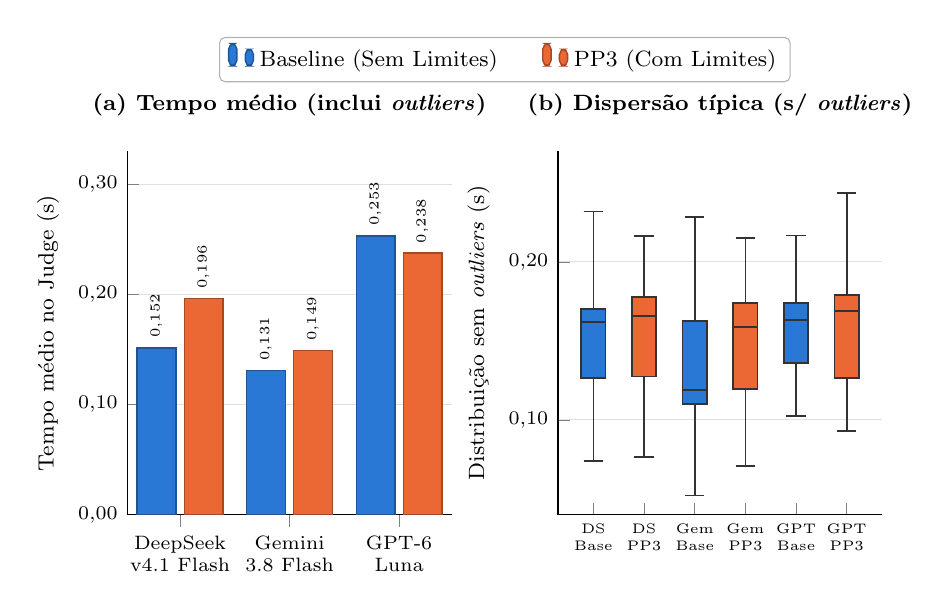
\begin{tikzpicture}
\begin{groupplot}[
  group style={
    group size=2 by 1,
    horizontal sep=1.35cm
  },
  width=0.47\textwidth,
  height=6.2cm,
  ymajorgrids=true,
  grid style={black!12},
  axis lines*=left,
  tick label style={font=\scriptsize},
  label style={font=\footnotesize},
  title style={font=\footnotesize\bfseries, yshift=3pt}
]
% Painel (a): Tempo médio no Judge
\nextgroupplot[
  ybar=3pt,
  bar width=14pt,
  symbolic x coords={DeepSeek,Gemini,GPT6},
  xtick={DeepSeek,Gemini,GPT6},
  xticklabels={DeepSeek\\v4.1 Flash,Gemini\\3.8 Flash,GPT-6\\Luna},
  x tick label style={align=center},
  enlarge x limits=0.24,
  ymin=0, ymax=0.33,
  ylabel={Tempo médio no Judge (s)},
  yticklabel style={/pgf/number format/fixed, /pgf/number format/fixed zerofill, /pgf/number format/precision=2, /pgf/number format/use comma},
  title={(a) Tempo médio (inclui \textit{outliers})},
  legend to name=legpp3tempo,
  legend style={
    legend columns=2,
    draw=black!30,
    rounded corners=2pt,
    font=\footnotesize,
    /tikz/every even column/.append style={column sep=14pt}
  },
  nodes near coords,
  nodes near coords style={
    font=\tiny\bfseries,
    black,
    rotate=90,
    anchor=west,
    /pgf/number format/fixed,
    /pgf/number format/fixed zerofill,
    /pgf/number format/precision=3,
    /pgf/number format/use comma
  }
]
\addplot[fill=vAzul, draw=vAzul!70!black, line width=0.5pt] coordinates {
  (DeepSeek,0.1515) (Gemini,0.1307) (GPT6,0.2531)
};
\addplot[fill=vLaranja, draw=vLaranja!70!black, line width=0.5pt] coordinates {
  (DeepSeek,0.1960) (Gemini,0.1489) (GPT6,0.2375)
};
\legend{Baseline (Sem Limites), PP3 (Com Limites)}

% Painel (b): Boxplot sem outliers (IQR + mediana)
\nextgroupplot[
  boxplot/draw direction=y,
  boxplot/box extend=0.48,
  xmin=0.3, xmax=6.7,
  ymin=0.04, ymax=0.27,
  xtick={1,2,3,4,5,6},
  xticklabels={DS\\Base,DS\\PP3,Gem\\Base,Gem\\PP3,GPT\\Base,GPT\\PP3},
  x tick label style={align=center, font=\tiny},
  ylabel={Distribuição sem \textit{outliers} (s)},
  yticklabel style={/pgf/number format/fixed, /pgf/number format/fixed zerofill, /pgf/number format/precision=2, /pgf/number format/use comma},
  title={(b) Dispersão típica (s/ \textit{outliers})}
]
% DeepSeek Base & PP3
\addplot+[boxplot prepared={
  draw position=1,
  lower whisker=0.0740, lower quartile=0.1263, median=0.1620, upper quartile=0.1701, upper whisker=0.2319
}, fill=vAzul, draw=black!80, line width=0.6pt, solid] coordinates {};
\addplot+[boxplot prepared={
  draw position=2,
  lower whisker=0.0767, lower quartile=0.1275, median=0.1659, upper quartile=0.1777, upper whisker=0.2163
}, fill=vLaranja, draw=black!80, line width=0.6pt, solid] coordinates {};
% Gemini Base & PP3
\addplot+[boxplot prepared={
  draw position=3,
  lower whisker=0.0522, lower quartile=0.1100, median=0.1190, upper quartile=0.1627, upper whisker=0.2285
}, fill=vAzul, draw=black!80, line width=0.6pt, solid] coordinates {};
\addplot+[boxplot prepared={
  draw position=4,
  lower whisker=0.0709, lower quartile=0.1197, median=0.1587, upper quartile=0.1740, upper whisker=0.2151
}, fill=vLaranja, draw=black!80, line width=0.6pt, solid] coordinates {};
% GPT-6 Luna Base & PP3
\addplot+[boxplot prepared={
  draw position=5,
  lower whisker=0.1023, lower quartile=0.1358, median=0.1633, upper quartile=0.1740, upper whisker=0.2166
}, fill=vAzul, draw=black!80, line width=0.6pt, solid] coordinates {};
\addplot+[boxplot prepared={
  draw position=6,
  lower whisker=0.0928, lower quartile=0.1267, median=0.1687, upper quartile=0.1789, upper whisker=0.2433
}, fill=vLaranja, draw=black!80, line width=0.6pt, solid] coordinates {};
\end{groupplot}

% Legenda compartilhada acima dos dois painéis
\node[anchor=south] at ($(group c1r1.north)!0.5!(group c2r1.north) + (0,0.75cm)$)
  {\pgfplotslegendfromname{legpp3tempo}};
\end{tikzpicture}

\caption[Tempos médios e distribuição de execução na PP3]{Análise de tempo no \textit{JudgeService} em \linguagem{C}: (a) tempo médio global (sensível a \textit{outliers}) e (b) distribuição por quartis e mediana sem \textit{outliers}.}
\label{fig:res-pp3-tempo}
\end{figure}
\FloatBarrier

Quanto ao consumo de \textit{tokens} e custo financeiro (Tabela~\ref{tab:res-pp3-custos} e Figura~\ref{fig:res-pp3-tokens-custo}), a inclusão das restrições adicionou cerca de 32 \textit{tokens} ao \textit{prompt} de entrada. No \textbf{DeepSeek v4.1 Flash}, a presença dos limites encurtou o raciocínio de saída em $13{,}3\%$ ($11.387{,}3 \rightarrow 9.870{,}5$ \textit{tokens}), reduzindo o custo por solução aceita de US\$\,0,00724 para US\$\,0,00628. Já no \textbf{GPT-6 Luna}, o código extra gerado para tentar otimizar as soluções elevou os \textit{tokens} de saída em $10{,}0\%$ e, somado à queda de 5 acertos, encareceu o custo por \veredito{AC} em $14{,}6\%$ (US\$\,0,00096 $\rightarrow$ US\$\,0,00110).

\begin{table}[!htbp]
\centering
\caption{Consumo médio de \textit{tokens}, custo total e custo por solução aceita em \linguagem{C} (\textit{Baseline} $\rightarrow$ \texttt{PP3}).}
\label{tab:res-pp3-custos}
\resizebox{\textwidth}{!}{%
\begin{tabular}{@{}lrrrr@{}}
\toprule
\textbf{LLM} & \textbf{Tokens Ent. (média)} & \textbf{Tokens Saída (média)} & \textbf{Custo Total (125 q.)} & \textbf{Custo por AC (US\$/AC)} \\
\midrule
DeepSeek v4.1 Flash & $891{,}9 \rightarrow 923{,}9$ ($+32{,}0$)  & $11.387{,}3 \rightarrow 9.870{,}5$ ($-1.516{,}8$) & \$0,8544 $\rightarrow$ \$0,7406 & \$0,00724 $\rightarrow$ \$0,00628 \\
Gemini 3.8 Flash    & $839{,}0 \rightarrow 873{,}2$ ($+34{,}2$)  & $531{,}8 \rightarrow 508{,}1$ ($-23{,}7$)        & \$0,3280 $\rightarrow$ \$0,3200 & \$0,00280 $\rightarrow$ \$0,00276 \\
GPT-6 Luna          & $781{,}2 \rightarrow 811{,}4$ ($+30{,}1$)  & $1.527{,}8 \rightarrow 1.681{,}0$ ($+153{,}1$)    & \$0,1053 $\rightarrow$ \$0,1152 & \$0,00096 $\rightarrow$ \$0,00110 \\
\bottomrule
\end{tabular}%
}
\end{table}

\begin{figure}[!htbp]
\centering
% Gráficos lado a lado: Tokens médios de saída e Custo por AC em C (Cap. 5, Seção 5.4.2)
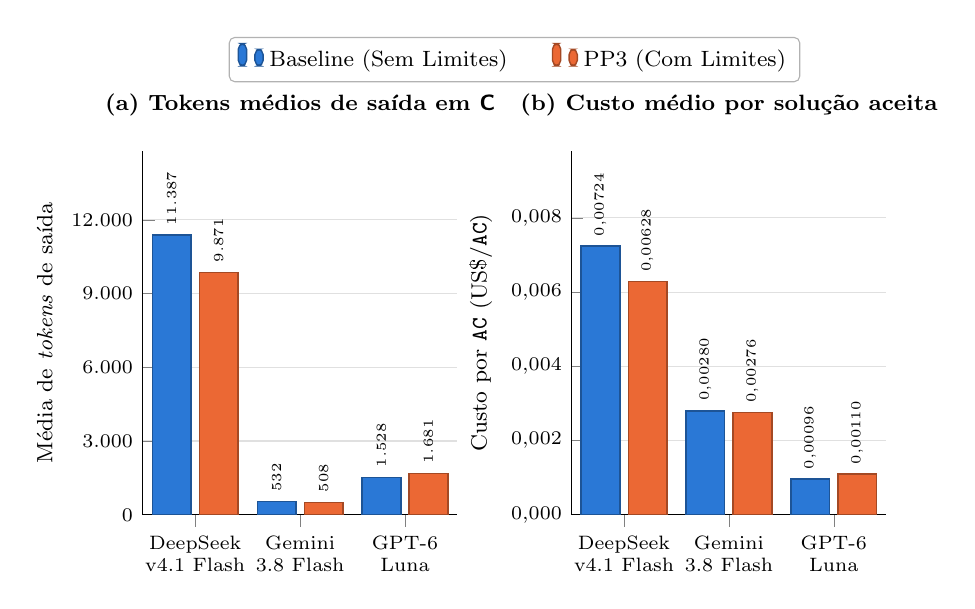
\begin{tikzpicture}
\begin{groupplot}[
  group style={
    group size=2 by 1,
    horizontal sep=1.45cm
  },
  width=0.46\textwidth,
  height=6.2cm,
  symbolic x coords={DeepSeek,Gemini,GPT6},
  xtick={DeepSeek,Gemini,GPT6},
  xticklabels={DeepSeek\\v4.1 Flash,Gemini\\3.8 Flash,GPT-6\\Luna},
  x tick label style={align=center},
  enlarge x limits=0.25,
  ymajorgrids=true,
  grid style={black!12},
  axis lines*=left,
  tick label style={font=\scriptsize},
  label style={font=\footnotesize},
  title style={font=\footnotesize\bfseries, yshift=3pt}
]
% Painel (a): Tokens médios de saída
\nextgroupplot[
  ybar=3pt,
  bar width=14pt,
  title={(a) Tokens médios de saída em \linguagem{C}},
  ymin=0, ymax=14800,
  scaled y ticks=false,
  ytick={0,3000,6000,9000,12000},
  ylabel={Média de \textit{tokens} de saída},
  yticklabel style={/pgf/number format/fixed, /pgf/number format/1000 sep={.}},
  legend to name=legpp3tokenscusto,
  legend style={
    legend columns=2,
    draw=black!30,
    rounded corners=2pt,
    font=\footnotesize,
    /tikz/every even column/.append style={column sep=14pt}
  },
  nodes near coords,
  nodes near coords style={
    font=\tiny\bfseries,
    black,
    rotate=90,
    anchor=west,
    /pgf/number format/fixed,
    /pgf/number format/precision=0,
    /pgf/number format/1000 sep={.}
  }
]
\addplot[fill=vAzul, draw=vAzul!70!black, line width=0.5pt] coordinates {
  (DeepSeek,11387.3) (Gemini,531.8) (GPT6,1527.8)
};
\addplot[fill=vLaranja, draw=vLaranja!70!black, line width=0.5pt] coordinates {
  (DeepSeek,9870.5) (Gemini,508.1) (GPT6,1681.0)
};
\legend{Baseline (Sem Limites), PP3 (Com Limites)}

% Painel (b): Custo por solução aceita (USD/AC)
\nextgroupplot[
  ybar=3pt,
  bar width=14pt,
  title={(b) Custo médio por solução aceita},
  ymin=0, ymax=0.0098,
  ylabel={Custo por \veredito{AC} (US\$/\veredito{AC})},
  ytick={0,0.002,0.004,0.006,0.008},
  yticklabel style={/pgf/number format/fixed, /pgf/number format/fixed zerofill, /pgf/number format/precision=3, /pgf/number format/use comma},
  scaled y ticks=false,
  nodes near coords,
  nodes near coords style={
    font=\tiny\bfseries,
    black,
    rotate=90,
    anchor=west,
    /pgf/number format/fixed,
    /pgf/number format/fixed zerofill,
    /pgf/number format/precision=5,
    /pgf/number format/use comma
  }
]
\addplot[fill=vAzul, draw=vAzul!70!black, line width=0.5pt] coordinates {
  (DeepSeek,0.00724) (Gemini,0.00280) (GPT6,0.00096)
};
\addplot[fill=vLaranja, draw=vLaranja!70!black, line width=0.5pt] coordinates {
  (DeepSeek,0.00628) (Gemini,0.00276) (GPT6,0.00110)
};
\end{groupplot}

% Legenda compartilhada acima dos dois gráficos
\node[anchor=south] at ($(group c1r1.north)!0.5!(group c2r1.north) + (0,0.75cm)$)
  {\pgfplotslegendfromname{legpp3tokenscusto}};
\end{tikzpicture}

\caption[Tokens de saída e custo por AC em C na PP3]{Telemetria em \linguagem{C} entre \textit{Baseline} e PP3: (a) média de \textit{tokens} de saída gerados por problema e (b) custo financeiro médio por solução aprovada (US\$/AC).}
\label{fig:res-pp3-tokens-custo}
\end{figure}
\FloatBarrier

\section{Detalhamento Complementar da PP4: Estratégias de \texorpdfstring{\textit{Prompting}}{Prompting} em C}\label{ap:pp4-detalhes}

\subsection{Decomposição de Erros e Desempenho por Fase da OBI}\label{sec:res-rq4-comp}

A Figura~\ref{fig:res-pp4-erros} ilustra a distribuição dos vereditos de erro (\veredito{WA}, \veredito{CE}, \veredito{RE} e \veredito{TLE}) correspondente à Tabela~\ref{tab:res-pp4-comparativo} discutida na Seção~\ref{sec:res-rq4}, evidenciando como o \promptname{Few-Shot} eliminou os erros de compilação no Gemini e no GPT-6 Luna, enquanto o \promptname{CoT Pólya} reduziu os erros de lógica (\veredito{WA}) nos três modelos.

\begin{figure}[!htbp]
\centering
% Gráfico em 3 painéis empilhados: taxonomia de erros (Não-AC) por estratégia em C (Cap. 5, Seção 5.5.1)
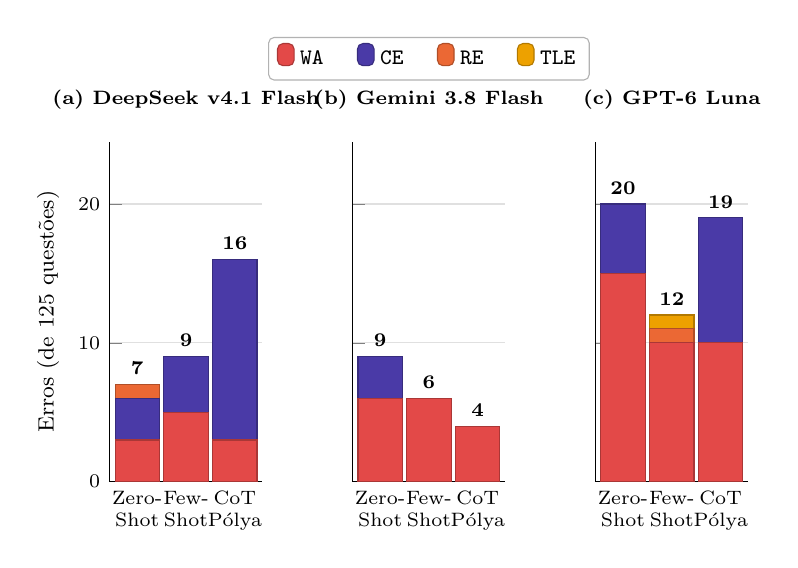
\begin{tikzpicture}
\begin{groupplot}[
  group style={
    group size=3 by 1,
    horizontal sep=1.15cm,
    yticklabels at=edge left
  },
  width=0.29\textwidth,
  height=5.9cm,
  symbolic x coords={Zero,Few,CoT},
  xtick={Zero,Few,CoT},
  xticklabels={Zero-\\Shot,Few-\\Shot,CoT\\Pólya},
  x tick label style={align=center},
  enlarge x limits=0.28,
  ymajorgrids=true,
  grid style={black!12},
  axis lines*=left,
  tick label style={font=\scriptsize},
  label style={font=\footnotesize},
  title style={font=\scriptsize\bfseries, yshift=2pt},
  ymin=0, ymax=24.5
]
% Painel (a): DeepSeek v4.1 Flash
\nextgroupplot[
  ybar stacked,
  bar width=16pt,
  title={(a) DeepSeek v4.1 Flash},
  ylabel={Erros (de 125 questões)},
  legend to name=legpp4erros,
  legend style={
    legend columns=4,
    draw=black!30,
    rounded corners=2pt,
    font=\footnotesize,
    /tikz/every even column/.append style={column sep=10pt}
  }
]
\addplot[fill=corWA, draw=corWA!75!black, line width=0.4pt] coordinates {(Zero,3) (Few,5) (CoT,3)};
\addplot[fill=corCE, draw=corCE!75!black, line width=0.4pt] coordinates {(Zero,3) (Few,4) (CoT,13)};
\addplot[fill=corRE, draw=corRE!75!black, line width=0.4pt] coordinates {(Zero,1) (Few,0) (CoT,0)};
\addplot[fill=corTLE, draw=corTLE!75!black, line width=0.4pt] coordinates {(Zero,0) (Few,0) (CoT,0)};
\legend{\veredito{WA}, \veredito{CE}, \veredito{RE}, \veredito{TLE}}
\node[font=\scriptsize\bfseries, anchor=south] at (axis cs:Zero,7) {7};
\node[font=\scriptsize\bfseries, anchor=south] at (axis cs:Few,9) {9};
\node[font=\scriptsize\bfseries, anchor=south] at (axis cs:CoT,16) {16};

% Painel (b): Gemini 3.8 Flash
\nextgroupplot[
  ybar stacked,
  bar width=16pt,
  title={(b) Gemini 3.8 Flash}
]
\addplot[fill=corWA, draw=corWA!75!black, line width=0.4pt] coordinates {(Zero,6) (Few,6) (CoT,4)};
\addplot[fill=corCE, draw=corCE!75!black, line width=0.4pt] coordinates {(Zero,3) (Few,0) (CoT,0)};
\addplot[fill=corRE, draw=corRE!75!black, line width=0.4pt] coordinates {(Zero,0) (Few,0) (CoT,0)};
\addplot[fill=corTLE, draw=corTLE!75!black, line width=0.4pt] coordinates {(Zero,0) (Few,0) (CoT,0)};
\node[font=\scriptsize\bfseries, anchor=south] at (axis cs:Zero,9) {9};
\node[font=\scriptsize\bfseries, anchor=south] at (axis cs:Few,6) {6};
\node[font=\scriptsize\bfseries, anchor=south] at (axis cs:CoT,4) {4};

% Painel (c): GPT-6 Luna
\nextgroupplot[
  ybar stacked,
  bar width=16pt,
  title={(c) GPT-6 Luna}
]
\addplot[fill=corWA, draw=corWA!75!black, line width=0.4pt] coordinates {(Zero,15) (Few,10) (CoT,10)};
\addplot[fill=corCE, draw=corCE!75!black, line width=0.4pt] coordinates {(Zero,5) (Few,0) (CoT,9)};
\addplot[fill=corRE, draw=corRE!75!black, line width=0.4pt] coordinates {(Zero,0) (Few,1) (CoT,0)};
\addplot[fill=corTLE, draw=corTLE!75!black, line width=0.4pt] coordinates {(Zero,0) (Few,1) (CoT,0)};
\node[font=\scriptsize\bfseries, anchor=south] at (axis cs:Zero,20) {20};
\node[font=\scriptsize\bfseries, anchor=south] at (axis cs:Few,12) {12};
\node[font=\scriptsize\bfseries, anchor=south] at (axis cs:CoT,19) {19};
\end{groupplot}

% Legenda compartilhada acima dos três painéis
\node[anchor=south] at ($(group c1r1.north)!0.5!(group c3r1.north) + (0,0.65cm)$)
  {\pgfplotslegendfromname{legpp4erros}};
\end{tikzpicture}

\caption[Decomposição de erros em C por estratégia na PP4]{Distribuição das submissões não aceitas em \linguagem{C} por veredito (\veredito{WA}, \veredito{CE}, \veredito{RE} e \veredito{TLE}) nas três estratégias de \textit{prompting}.}
\label{fig:res-pp4-erros}
\end{figure}
\FloatBarrier

Para avaliar em qual nível de dificuldade das provas cada técnica trouxe maior benefício, a Tabela~\ref{tab:res-pp4-fases} estratifica a taxa média de acerto nas edições rotuladas diretamente como \textit{Fase~1} ($n=27$), \textit{Fase~2} ($n=32$) e \textit{Fase~3} ($n=25$), além de contabilizar o balanço de questões recuperadas e degradadas frente ao \textit{Zero-Shot}. Nota-se que o maior salto ocorreu nas questões intermediárias da \textit{Fase~2}, onde tanto o \promptname{Few-Shot} quanto o \promptname{CoT Pólya} elevaram a média de $89{,}58\%$ para $97{,}92\%$ ($+8{,}34\text{ p.p.}$). No balanço individual, o \textbf{Gemini 3.8 Flash} com \promptname{CoT Pólya} recuperou 5 questões sem sofrer nenhuma regressão ($+5/-0$), e o \textbf{GPT-6 Luna} recuperou 12 questões em ambas as técnicas guiadas.

\begin{table}[!htbp]
\centering
\caption{Taxa média de aprovação (\passat{1}) por fase da OBI Sênior em \linguagem{C} e balanço de transições frente ao \textit{Zero-Shot}.}
\label{tab:res-pp4-fases}
\resizebox{\textwidth}{!}{%
\begin{tabular}{@{}lccc|lcc@{}}
\toprule
\textbf{Fase da OBI} & \textbf{\textit{Zero-Shot}} & \textbf{\textit{Few-Shot}} & \textbf{\textit{CoT Pólya}} & \textbf{LLM (Balanço Rec. / Deg.)} & \textbf{\textit{Few-Shot}} & \textbf{\textit{CoT Pólya}} \\
\midrule
Fase 1 ($n=27$) & $100{,}00\%$ & $100{,}00\%$ & $93{,}83\%$ & DeepSeek v4.1 Flash & $+4 / -6$ ($-2$)  & $+4 / -13$ ($-9$) \\
Fase 2 ($n=32$) & $89{,}58\%$  & \tfirst{97,92\%} & \tfirst{97,92\%} & Gemini 3.8 Flash    & $+4 / -1$ ($+3$)  & \tfirst{$+5 / -0$ ($+5$)} \\
Fase 3 ($n=25$) & $81{,}33\%$  & $80{,}00\%$  & $74{,}67\%$ & GPT-6 Luna          & \tfirst{$+12 / -4$ ($+8$)} & $+12 / -11$ ($+1$) \\
\bottomrule
\end{tabular}%
}
\par\smallskip{\footnotesize Colunas à esquerda consideram as edições rotuladas literalmente como \texttt{Fase 1}, \texttt{Fase 2} e \texttt{Fase 3}; à direita, o número de questões recuperadas (Rec.) e degradadas (Deg.) frente ao \textit{Zero-Shot}.}
\end{table}

\subsection{Auditoria dos Erros de Extração no \textit{CoT Pólya}}\label{sec:res-rq4-parser}

Conforme apontado na Seção~\ref{sec:res-rq4}, o aumento de erros de compilação (\veredito{CE}) no \promptname{CoT Pólya} para o \textbf{DeepSeek v4.1 Flash} (13 casos) e para o \textbf{GPT-6 Luna} (9 casos) motivou uma auditoria direta sobre o campo \texttt{raw\_response} dos arquivos JSON de saída. Como o roteiro de Pólya pede que o modelo escreva quatro seções analíticas, essas respostas frequentemente continham blocos Markdown auxiliares (com rascunhos de entrada/saída ou análise na etapa 4) além do bloco \texttt{\textasciigrave\textasciigrave\textasciigrave c ... \textasciigrave\textasciigrave\textasciigrave}, fazendo o extrator baseado no maior bloco genérico capturar texto explicativo em vez do programa em \linguagem{C}.

A Tabela~\ref{tab:res-pp4-parser} resume o resultado dessa verificação sobre os 22 casos de \veredito{CE}. No \textbf{GPT-6 Luna}, 8 das 9 falhas ($88{,}9\%$) continham um programa \linguagem{C} completo com função \texttt{main()} dentro da resposta bruta; no \textbf{DeepSeek v4.1 Flash}, 6 dos 13 casos ($46{,}2\%$) também traziam código \linguagem{C} completo, enquanto outros 5 retornaram objetos JSON estruturados em texto e 2 estouraram o limite de saída. Se o extrator filtrasse estritamente blocos marcados com a linguagem-alvo (\texttt{\textasciigrave\textasciigrave\textasciigrave c}) contendo \texttt{main()}, o GPT-6 Luna poderia alcançar até $91{,}20\%$ ($114/125$) e o DeepSeek até $92{,}00\%$ ($115/125$).

\begin{table}[!htbp]
\centering
\caption{Auditoria dos $22$ casos de \veredito{CE} sob \promptname{CoT Pólya} em \linguagem{C}: códigos válidos ocultos e impacto potencial.}
\label{tab:res-pp4-parser}
\resizebox{\textwidth}{!}{%
\begin{tabular}{@{}lcccp{5.4cm}cc@{}}
\toprule
\textbf{LLM} & \textbf{Total CE} & \textbf{Cód. \texttt{main()}} & \textbf{JSON / Inc.} & \textbf{Questões com Código C Oculto} & \textbf{\passat{1} Bruto} & \textbf{Teto Ajustado*} \\
\midrule
DeepSeek v4.1 Flash & $13$ & $6$ ($46{,}2\%$) & $5$ JSON, $2$ vazios & \textit{Botas Trocadas}, \textit{Camisetas da Olimpíada}, \textit{Chuva\_2022}, \textit{Construção de Rodovia}, \textit{Fotos de Relíquias}, \textit{Remove Dígitos} & $87{,}20\%$ ($109$) & até $92{,}00\%$ ($115$) \\
GPT-6 Luna          & $9$  & $8$ ($88{,}9\%$) & $1$ truncado         & \textit{Fast-Food}, \textit{Festa Junina}, \textit{Festa olímpica}, \textit{Game-10}, \textit{Pirâmide}, \textit{Quadrado}, \textit{Soma}, \textit{Trem da mina} & $84{,}80\%$ ($106$) & até $91{,}20\%$ ($114$) \\
\bottomrule
\end{tabular}%
}
\par\smallskip{\footnotesize *Teto ajustado calculado somando ao \passat{1} bruto os casos que continham bloco \texttt{\textasciigrave\textasciigrave\textasciigrave c} válido com função \texttt{main()}, caso extraídos corretamente e aprovados pelo juiz.}
\end{table}

\subsection{Tempos de Execução e Comparativo Visual de Custos na PP4}\label{sec:res-rq4-economia}

As Figuras~\ref{fig:res-pp4-tempo} e~\ref{fig:res-pp4-tokens-custo} complementam a análise de eficiência da Seção~\ref{sec:res-rq4}. Na Figura~\ref{fig:res-pp4-tempo}, observa-se que as medianas de tempo de CPU das soluções aprovadas permaneceram praticamente idênticas nas três estratégias ($\approx 0{,}16\,\mathrm{s}$). Já a Figura~\ref{fig:res-pp4-tokens-custo} permite visualizar o contraste econômico reportado na Tabela~\ref{tab:res-pp4-custos}: o \promptname{Few-Shot} manteve a quantidade de \textit{tokens} de saída contida (chegando a reduzi-la em $18{,}4\%$ no GPT-6 Luna), enquanto o \promptname{CoT Pólya} elevou a geração textual no Gemini e no GPT-6 Luna devido à escrita das quatro etapas de Pólya.

\begin{figure}[!htbp]
\centering
% Gráficos lado a lado: Tempo médio global e Boxplot (AC sem outliers) por estratégia em C (Cap. 5, Seção 5.5.3)
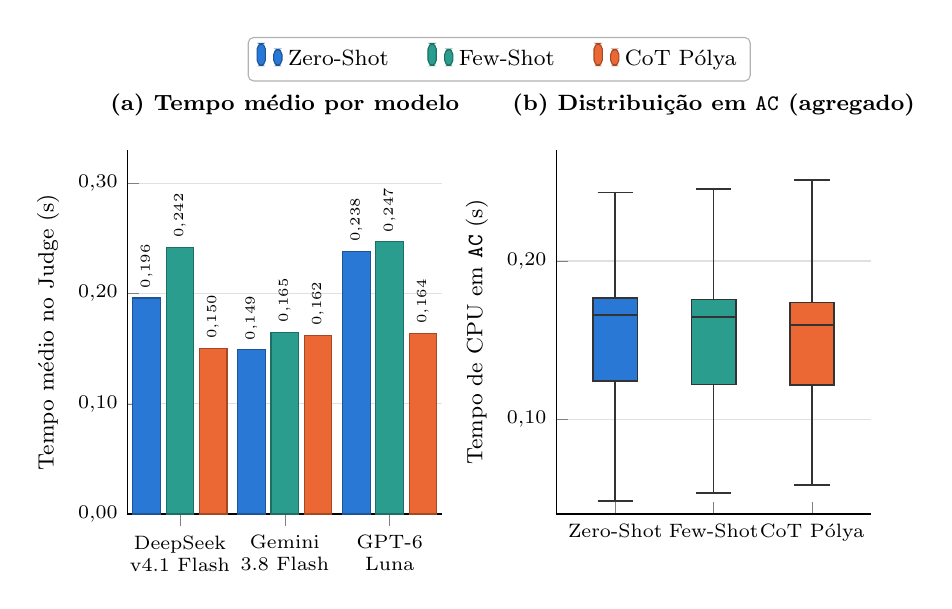
\begin{tikzpicture}
\begin{groupplot}[
  group style={
    group size=2 by 1,
    horizontal sep=1.45cm
  },
  width=0.46\textwidth,
  height=6.2cm,
  ymajorgrids=true,
  grid style={black!12},
  axis lines*=left,
  tick label style={font=\scriptsize},
  label style={font=\footnotesize},
  title style={font=\footnotesize\bfseries, yshift=3pt}
]
% Painel (a): Tempo médio global por estratégia e LLM
\nextgroupplot[
  ybar=2pt,
  bar width=10pt,
  symbolic x coords={DeepSeek,Gemini,GPT6},
  xtick={DeepSeek,Gemini,GPT6},
  xticklabels={DeepSeek\\v4.1 Flash,Gemini\\3.8 Flash,GPT-6\\Luna},
  x tick label style={align=center},
  enlarge x limits=0.25,
  ymin=0, ymax=0.33,
  ylabel={Tempo médio no Judge (s)},
  yticklabel style={/pgf/number format/fixed, /pgf/number format/fixed zerofill, /pgf/number format/precision=2, /pgf/number format/use comma},
  title={(a) Tempo médio por modelo},
  legend to name=legpp4tempo,
  legend style={
    legend columns=3,
    draw=black!30,
    rounded corners=2pt,
    font=\footnotesize,
    /tikz/every even column/.append style={column sep=12pt}
  },
  nodes near coords,
  nodes near coords style={
    font=\tiny\bfseries,
    black,
    rotate=90,
    anchor=west,
    /pgf/number format/fixed,
    /pgf/number format/fixed zerofill,
    /pgf/number format/precision=3,
    /pgf/number format/use comma
  }
]
\addplot[fill=vAzul, draw=vAzul!70!black, line width=0.4pt] coordinates {
  (DeepSeek,0.196) (Gemini,0.149) (GPT6,0.238)
};
\addplot[fill=vTeal, draw=vTeal!70!black, line width=0.4pt] coordinates {
  (DeepSeek,0.242) (Gemini,0.165) (GPT6,0.247)
};
\addplot[fill=vLaranja, draw=vLaranja!70!black, line width=0.4pt] coordinates {
  (DeepSeek,0.150) (Gemini,0.162) (GPT6,0.164)
};
\legend{Zero-Shot, Few-Shot, CoT Pólya}

% Painel (b): Boxplot sem outliers das soluções AC (agregado das 3 LLMs)
\nextgroupplot[
  boxplot/draw direction=y,
  boxplot/box extend=0.45,
  xmin=0.4, xmax=3.6,
  ymin=0.04, ymax=0.27,
  xtick={1,2,3},
  xticklabels={Zero-Shot,Few-Shot,CoT Pólya},
  x tick label style={align=center, font=\scriptsize},
  ylabel={Tempo de CPU em \veredito{AC} (s)},
  yticklabel style={/pgf/number format/fixed, /pgf/number format/fixed zerofill, /pgf/number format/precision=2, /pgf/number format/use comma},
  title={(b) Distribuição em \veredito{AC} (agregado)}
]
\addplot+[boxplot prepared={
  draw position=1,
  lower whisker=0.0482, lower quartile=0.1243, median=0.1659, upper quartile=0.1766, upper whisker=0.2433
}, fill=vAzul, draw=black!80, line width=0.6pt, solid] coordinates {};
\addplot+[boxplot prepared={
  draw position=2,
  lower whisker=0.0533, lower quartile=0.1219, median=0.1646, upper quartile=0.1757, upper whisker=0.2454
}, fill=vTeal, draw=black!80, line width=0.6pt, solid] coordinates {};
\addplot+[boxplot prepared={
  draw position=3,
  lower whisker=0.0582, lower quartile=0.1214, median=0.1597, upper quartile=0.1737, upper whisker=0.2513
}, fill=vLaranja, draw=black!80, line width=0.6pt, solid] coordinates {};
\end{groupplot}

% Legenda compartilhada acima dos dois painéis
\node[anchor=south] at ($(group c1r1.north)!0.5!(group c2r1.north) + (0,0.75cm)$)
  {\pgfplotslegendfromname{legpp4tempo}};
\end{tikzpicture}

\caption[Tempos médios e distribuição AC por estratégia na PP4]{Desempenho em CPU no \textit{JudgeService} em \linguagem{C}: (a) tempo médio global por modelo e estratégia e (b) boxplot agregado dos tempos de soluções aprovadas (\veredito{AC}, sem \textit{outliers}).}
\label{fig:res-pp4-tempo}
\end{figure}

\begin{figure}[!htbp]
\centering
% Gráficos lado a lado: Tokens médios de saída e Custo por AC por estratégia em C (Cap. 5, Seção 5.5.3)
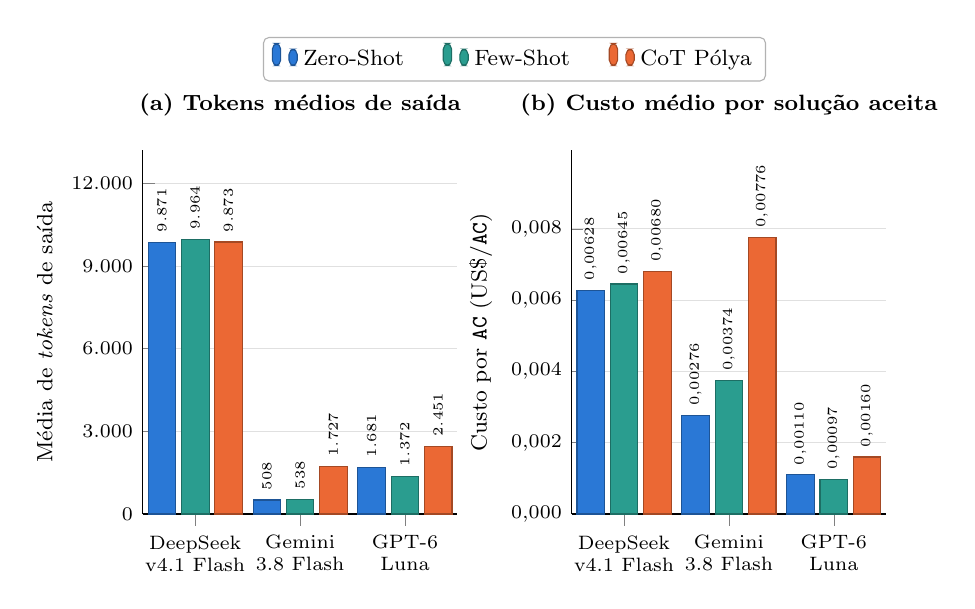
\begin{tikzpicture}
\begin{groupplot}[
  group style={
    group size=2 by 1,
    horizontal sep=1.45cm
  },
  width=0.46\textwidth,
  height=6.2cm,
  symbolic x coords={DeepSeek,Gemini,GPT6},
  xtick={DeepSeek,Gemini,GPT6},
  xticklabels={DeepSeek\\v4.1 Flash,Gemini\\3.8 Flash,GPT-6\\Luna},
  x tick label style={align=center},
  enlarge x limits=0.25,
  ymajorgrids=true,
  grid style={black!12},
  axis lines*=left,
  tick label style={font=\scriptsize},
  label style={font=\footnotesize},
  title style={font=\footnotesize\bfseries, yshift=3pt}
]
% Painel (a): Tokens médios de saída
\nextgroupplot[
  ybar=2pt,
  bar width=10pt,
  title={(a) Tokens médios de saída},
  ymin=0, ymax=13200,
  scaled y ticks=false,
  ytick={0,3000,6000,9000,12000},
  ylabel={Média de \textit{tokens} de saída},
  yticklabel style={/pgf/number format/fixed, /pgf/number format/1000 sep={.}},
  legend to name=legpp4tokenscusto,
  legend style={
    legend columns=3,
    draw=black!30,
    rounded corners=2pt,
    font=\footnotesize,
    /tikz/every even column/.append style={column sep=12pt}
  },
  nodes near coords,
  nodes near coords style={
    font=\tiny\bfseries,
    black,
    rotate=90,
    anchor=west,
    /pgf/number format/fixed,
    /pgf/number format/precision=0,
    /pgf/number format/1000 sep={.}
  }
]
\addplot[fill=vAzul, draw=vAzul!70!black, line width=0.4pt] coordinates {
  (DeepSeek,9870.5) (Gemini,508.1) (GPT6,1681.0)
};
\addplot[fill=vTeal, draw=vTeal!70!black, line width=0.4pt] coordinates {
  (DeepSeek,9964.2) (Gemini,537.9) (GPT6,1371.6)
};
\addplot[fill=vLaranja, draw=vLaranja!70!black, line width=0.4pt] coordinates {
  (DeepSeek,9872.7) (Gemini,1726.8) (GPT6,2450.7)
};
\legend{Zero-Shot, Few-Shot, CoT Pólya}

% Painel (b): Custo médio por solução aceita (USD/AC)
\nextgroupplot[
  ybar=2pt,
  bar width=10pt,
  title={(b) Custo médio por solução aceita},
  ymin=0, ymax=0.0102,
  ylabel={Custo por \veredito{AC} (US\$/\veredito{AC})},
  ytick={0,0.002,0.004,0.006,0.008},
  yticklabel style={/pgf/number format/fixed, /pgf/number format/fixed zerofill, /pgf/number format/precision=3, /pgf/number format/use comma},
  scaled y ticks=false,
  nodes near coords,
  nodes near coords style={
    font=\tiny\bfseries,
    black,
    rotate=90,
    anchor=west,
    /pgf/number format/fixed,
    /pgf/number format/fixed zerofill,
    /pgf/number format/precision=5,
    /pgf/number format/use comma
  }
]
\addplot[fill=vAzul, draw=vAzul!70!black, line width=0.4pt] coordinates {
  (DeepSeek,0.00628) (Gemini,0.00276) (GPT6,0.00110)
};
\addplot[fill=vTeal, draw=vTeal!70!black, line width=0.4pt] coordinates {
  (DeepSeek,0.00645) (Gemini,0.00374) (GPT6,0.00097)
};
\addplot[fill=vLaranja, draw=vLaranja!70!black, line width=0.4pt] coordinates {
  (DeepSeek,0.00680) (Gemini,0.00776) (GPT6,0.00160)
};
\end{groupplot}

% Legenda compartilhada acima dos dois gráficos
\node[anchor=south] at ($(group c1r1.north)!0.5!(group c2r1.north) + (0,0.75cm)$)
  {\pgfplotslegendfromname{legpp4tokenscusto}};
\end{tikzpicture}

\caption[Tokens de saída e custo por AC por estratégia na PP4]{Análise econômica das estratégias de \textit{prompting} em \linguagem{C}: (a) média de \textit{tokens} de saída por resposta e (b) custo financeiro médio por solução aceita (US\$/AC).}
\label{fig:res-pp4-tokens-custo}
\end{figure}
\FloatBarrier

\section{Detalhamento Complementar da PP5: Evolução Geracional sob Paridade de Juiz}\label{ap:pp5-detalhes}

\subsection{Desempenho Detalhado por Modelo e Efeito da Paridade de Juiz}\label{sec:res-rq5-pass1}

A Tabela~\ref{tab:res-pp5-consolidado} e a Figura~\ref{fig:res-pp5-pass1-erros} detalham os indicadores individuais dos quatro modelos comparados nas 46 questões em \linguagem{Python} \textit{Zero-Shot}, complementando a síntese intrafamília apresentada na Tabela~\ref{tab:res-pp5-intrafamilia} do Capítulo~\ref{cap:resultados}.

\begin{table}[!htbp]
\centering
\caption[Desempenho consolidado na PP5 sob paridade de juiz]{Desempenho consolidado dos quatro modelos nas $46$ questões em \linguagem{Python} \textit{Zero-Shot} ($T = 0{,}0$) sob o mesmo \texttt{JudgeService}.}
\label{tab:res-pp5-consolidado}
\small
\resizebox{\textwidth}{!}{%
\begin{tabular}{@{}lllcccccccrrr@{}}
\toprule
\textbf{Modelo} & \textbf{Família} & \textbf{Geração} & \textbf{AC} & \textbf{\passat{1}} & \textbf{WA} & \textbf{RE} & \textbf{TLE} & \textbf{CE} & \textbf{Tokens Méd.} & \textbf{Custo Total} & \textbf{Custo / AC} \\
\midrule
Gemini 3.1 Pro   & Gemini & Anterior & \tfirst{45}  & \tfirst{97,83\%}  & $1$  & $0$ & $0$ & $0$ & $6.025{,}5$ & \$2,8602 & \$0,06356 \\
Gemini 3.8 Flash & Gemini & Atual    & \tsecond{44} & \tsecond{95,65\%} & $2$  & $0$ & $0$ & $0$ & $2.940{,}4$ & \$0,0994 & \tsecond{\$0,00226} \\
\midrule
GPT-5.4          & GPT    & Anterior & $31$         & $67{,}39\%$       & $12$ & $2$ & $1$ & $0$ & \tfirst{$1.206{,}4$} & \$0,3013 & \$0,00972 \\
GPT-6 Luna       & GPT    & Atual    & $38$         & $82{,}61\%$       & $6$  & $0$ & $2$ & $0$ & \tsecond{$2.044{,}9$} & \tfirst{\$0,0316} & \tfirst{\$0,00083} \\
\bottomrule
\end{tabular}%
}
\par\smallskip{\footnotesize \tfirst{Vermelho} e \tsecond{azul}: melhor e segundo melhor valor nos indicadores-chave.}
\end{table}

\begin{figure}[!htbp]
\centering
% Gráfico em 2 painéis: Pass@1 (%) e Taxonomia de Falhas (Não-AC) na PP5 (Cap. 5, Seção 5.6.1)
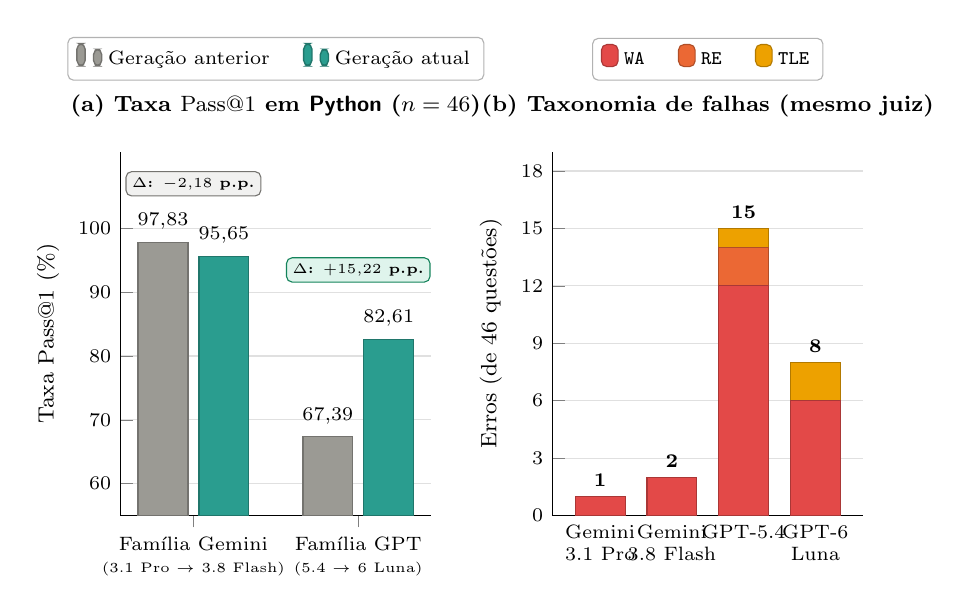
\begin{tikzpicture}
\begin{groupplot}[
  group style={
    group size=2 by 1,
    horizontal sep=1.55cm
  },
  width=0.455\textwidth,
  height=6.2cm,
  ymajorgrids=true,
  grid style={black!12},
  axis lines*=left,
  tick label style={font=\scriptsize},
  label style={font=\footnotesize},
  title style={font=\footnotesize\bfseries, yshift=3pt}
]
% Painel (a): Taxa Pass@1 (%) comparando geração anterior vs. geração atual por família
\nextgroupplot[
  ybar=4pt,
  bar width=18pt,
  clip=false,
  title={(a) Taxa \passat{1} em \linguagem{Python} ($n=46$)},
  symbolic x coords={Gemini,GPT},
  xtick={Gemini,GPT},
  xticklabels={Família Gemini\\{\tiny (3.1 Pro $\rightarrow$ 3.8 Flash)},Família GPT\\{\tiny (5.4 $\rightarrow$ 6 Luna)}},
  x tick label style={align=center},
  enlarge x limits=0.44,
  ymin=55, ymax=112,
  ytick={60,70,80,90,100},
  ylabel={Taxa \passat{1} (\%)},
  legend to name=legpp5pass1,
  legend style={
    legend columns=2,
    draw=black!30,
    rounded corners=2pt,
    font=\scriptsize,
    /tikz/every even column/.append style={column sep=10pt}
  },
  nodes near coords,
  nodes near coords style={
    font=\scriptsize\bfseries,
    black,
    yshift=1pt,
    /pgf/number format/fixed,
    /pgf/number format/fixed zerofill,
    /pgf/number format/precision=2,
    /pgf/number format/use comma
  }
]
\addplot[fill=vCinza, draw=vCinza!75!black, line width=0.5pt] coordinates {
  (Gemini,97.83) (GPT,67.39)
};
\addplot[fill=vTeal, draw=vTeal!75!black, line width=0.5pt] coordinates {
  (Gemini,95.65) (GPT,82.61)
};
\legend{Geração anterior, Geração atual}

% Pílulas com a variação (Delta) acima de cada par
\node[font=\tiny\bfseries, fill=vCinza!14, draw=vCinza!75!black, rounded corners=2pt, inner sep=2.2pt]
  at (axis cs:Gemini,107.0) {$\Delta$: $-2{,}18$ p.p.};
\node[font=\tiny\bfseries, fill=vVerde!14, draw=vVerde!75!black, rounded corners=2pt, inner sep=2.2pt]
  at (axis cs:GPT,93.5) {$\Delta$: $+15{,}22$ p.p.};

% Painel (b): Taxonomia de erros (Não-AC) sob o mesmo JudgeService
\nextgroupplot[
  ybar stacked,
  bar width=18pt,
  title={(b) Taxonomia de falhas (mesmo juiz)},
  symbolic x coords={G31,G38,GPT54,GPT6},
  xtick={G31,G38,GPT54,GPT6},
  xticklabels={Gemini\\3.1 Pro,Gemini\\3.8 Flash,GPT-5.4,GPT-6\\Luna},
  x tick label style={align=center},
  enlarge x limits=0.22,
  ymin=0, ymax=19,
  ytick={0,3,6,9,12,15,18},
  ylabel={Erros (de 46 questões)},
  legend to name=legpp5erros,
  legend style={
    legend columns=3,
    draw=black!30,
    rounded corners=2pt,
    font=\scriptsize,
    /tikz/every even column/.append style={column sep=10pt}
  }
]
\addplot[fill=corWA, draw=corWA!75!black, line width=0.4pt] coordinates {
  (G31,1) (G38,2) (GPT54,12) (GPT6,6)
};
\addplot[fill=corRE, draw=corRE!75!black, line width=0.4pt] coordinates {
  (G31,0) (G38,0) (GPT54,2) (GPT6,0)
};
\addplot[fill=corTLE, draw=corTLE!75!black, line width=0.4pt] coordinates {
  (G31,0) (G38,0) (GPT54,1) (GPT6,2)
};
\legend{\veredito{WA}, \veredito{RE}, \veredito{TLE}}

% Totais acima de cada barra empilhada
\node[font=\scriptsize\bfseries, anchor=south] at (axis cs:G31,1) {1};
\node[font=\scriptsize\bfseries, anchor=south] at (axis cs:G38,2) {2};
\node[font=\scriptsize\bfseries, anchor=south] at (axis cs:GPT54,15) {15};
\node[font=\scriptsize\bfseries, anchor=south] at (axis cs:GPT6,8) {8};
\end{groupplot}

% Legendas individuais acima de cada painel
\node[anchor=south] at ($(group c1r1.north) + (0,0.78cm)$)
  {\pgfplotslegendfromname{legpp5pass1}};
\node[anchor=south] at ($(group c2r1.north) + (0,0.78cm)$)
  {\pgfplotslegendfromname{legpp5erros}};
\end{tikzpicture}

\caption[Pass@1 e taxonomia de falhas na PP5]{Comparação entre gerações nas $46$ questões em \linguagem{Python} \textit{Zero-Shot} ($T=0$): (a) taxa \passat{1} intrafamília com variação em pontos percentuais e (b) composição dos erros sob o mesmo \texttt{JudgeService}.}
\label{fig:res-pp5-pass1-erros}
\end{figure}
\FloatBarrier

A inspeção dos vereditos mostra por que o rejulgamento dos códigos da geração anterior no mesmo \texttt{JudgeService} foi indispensável. Na avaliação original do estudo preliminar, o teto fixo de $3{,}0\,\mathrm{s}$ para \linguagem{Python} havia gerado falsos \veredito{TLE} em problemas cujo limite oficial da OBI é de $5{,}0\,\mathrm{s}$, como \textit{Brigadeiros} (no Gemini 3.1 Pro) e \textit{Transportes} (em ambos os modelos anteriores). De forma semelhante, a comparação de saída sem remoção de espaços ao final de cada linha havia penalizado a questão \textit{Pirâmide} (2022) com falso \veredito{WA}. Com a paridade de juiz, o \textbf{Gemini 3.1 Pro} subiu de 42 para 45 acertos e o \textbf{GPT-5.4} passou de 29 para 31 acertos, garantindo que a evolução reportada para o \textbf{GPT-6 Luna} ($38/46$, com redução de \veredito{WA} de 12 para 6 e zeramento dos \veredito{RE}s) represente um ganho real de geração de código.

Quanto à contabilização financeira na família Google, cabe registrar que o custo retornado pela API para o \textbf{Gemini 3.8 Flash} (US\$\,0,0994 no total, ou US\$\,0,00226 por \veredito{AC}) incide sobre os \textit{tokens} visíveis de entrada e saída, enquanto o total de \textit{tokens} reportado na Tabela~\ref{tab:res-pp5-consolidado} inclui $75.571$ \textit{thinking tokens} internos ao longo das 46 questões. Mesmo que todos esses \textit{tokens} internos fossem tarifados pelo valor cheio de saída (US\$\,3,75 por milhão), o custo subiria para US\$\,0,3828 (US\$\,0,00870 por \veredito{AC}), ainda $7{,}3$ vezes menor que o do \textbf{Gemini 3.1 Pro}.

\subsection{Mapeamento das Questões com Divergência entre Gerações}\label{sec:res-rq5-fases}

Das 46 questões avaliadas na PP5, 30 ($65{,}22\%$) obtiveram aprovação unânime nos quatro modelos. As 16 questões em que ocorreu falha ou mudança de veredito entre gerações são apresentadas na Tabela~\ref{tab:res-pp5-divergentes}.

\begin{table}[!htbp]
\centering
\caption[Questões com falha ou divergência entre os quatro modelos na PP5]{Vereditos nas $16$ questões em que ao menos um dos quatro modelos não obteve \veredito{AC} em \linguagem{Python} \textit{Zero-Shot} ($T = 0{,}0$).}
\label{tab:res-pp5-divergentes}
\small
\resizebox{\textwidth}{!}{%
\begin{tabular}{@{}cllcccc@{}}
\toprule
\textbf{Ano} & \textbf{Questão} & \textbf{Etapa} & \textbf{Gemini 3.1 Pro} & \textbf{Gemini 3.8 Flash} & \textbf{GPT-5.4} & \textbf{GPT-6 Luna} \\
\midrule
2016 & Arco e flecha         & Fase 2 / Estadual & \veredito{AC} & \veredito{WA} & \veredito{RE}  & \veredito{AC}  \\
2016 & Nova avenida          & Fase 1 / Local    & \veredito{AC} & \veredito{AC} & \veredito{WA}  & \veredito{AC}  \\
2017 & Cortando o Papel      & Fase 2 / Estadual & \veredito{AC} & \veredito{AC} & \veredito{WA}  & \veredito{AC}  \\
2017 & Dario e Xerxes        & Fase 2 / Estadual & \veredito{AC} & \veredito{AC} & \veredito{WA}  & \veredito{WA}  \\
2019 & Calçada Imperial      & Fase 1 / Local    & \veredito{AC} & \veredito{AC} & \veredito{WA}  & \veredito{AC}  \\
2019 & Chuva\_2019           & Fase 1 / Local    & \veredito{AC} & \veredito{AC} & \veredito{TLE} & \veredito{WA}  \\
2019 & Metrô da Nlogônia     & Fase 3 / Nacional & \veredito{AC} & \veredito{AC} & \veredito{WA}  & \veredito{AC}  \\
2021 & Dona Minhoca          & Fase 3 / Nacional & \veredito{AC} & \veredito{AC} & \veredito{WA}  & \veredito{WA}  \\
2021 & Retângulo             & Fase 2 / Estadual & \veredito{AC} & \veredito{AC} & \veredito{WA}  & \veredito{AC}  \\
2022 & Construção de Rodovia & Fase 3 / Nacional & \veredito{WA} & \veredito{WA} & \veredito{WA}  & \veredito{WA}  \\
2023 & Fast-Food             & Fase 3 / Nacional & \veredito{AC} & \veredito{AC} & \veredito{WA}  & \veredito{TLE} \\
2023 & Trio de Bonecas       & Fase 3 / Nacional & \veredito{AC} & \veredito{AC} & \veredito{WA}  & \veredito{TLE} \\
2024 & Brigadeiros           & Fase 3 / Nacional & \veredito{AC} & \veredito{AC} & \veredito{WA}  & \veredito{AC}  \\
2024 & Burocracia            & Fase 3 / Nacional & \veredito{AC} & \veredito{AC} & \veredito{RE}  & \veredito{WA}  \\
2024 & Jogo da Vida          & Fase 1 / Local    & \veredito{AC} & \veredito{AC} & \veredito{AC}  & \veredito{WA}  \\
2024 & Retas                 & Fase 3 / Nacional & \veredito{AC} & \veredito{AC} & \veredito{WA}  & \veredito{AC}  \\
\bottomrule
\end{tabular}%
}
\par\smallskip{\footnotesize Nas demais $30$ questões ($65{,}22\%$), houve \veredito{AC} unânime.}
\end{table}

A comparação nominal mostra que a família Google manteve estabilidade quase total, registrando apenas uma regressão em \textit{Arco e flecha} (\veredito{AC} $\rightarrow$ \veredito{WA}). Já na família OpenAI, o \textbf{GPT-6 Luna} recuperou 8 problemas que o \textbf{GPT-5.4} havia errado --- com destaque para questões da Fase~2 (\textit{Arco e flecha}, \textit{Cortando o Papel} e \textit{Retângulo}) e da Fase~3 (\textit{Brigadeiros}, \textit{Metrô da Nlogônia} e \textit{Retas}) --- e apresentou apenas uma regressão pontual (\textit{Jogo da Vida}). A única questão sem solução em nenhum dos quatro modelos foi \textit{Construção de Rodovia} (2022), que admite múltiplos pares de saída válidos sem verificador customizado (\textit{special judge}) na base oficial.
\FloatBarrier


\end{document}
